% Options for packages loaded elsewhere
\PassOptionsToPackage{unicode}{hyperref}
\PassOptionsToPackage{hyphens}{url}
\PassOptionsToPackage{dvipsnames,svgnames,x11names}{xcolor}
%
\documentclass[
  letterpaper,
  DIV=11,
  numbers=noendperiod]{scrreprt}

\usepackage{amsmath,amssymb}
\usepackage{iftex}
\ifPDFTeX
  \usepackage[T1]{fontenc}
  \usepackage[utf8]{inputenc}
  \usepackage{textcomp} % provide euro and other symbols
\else % if luatex or xetex
  \usepackage{unicode-math}
  \defaultfontfeatures{Scale=MatchLowercase}
  \defaultfontfeatures[\rmfamily]{Ligatures=TeX,Scale=1}
\fi
\usepackage{lmodern}
\ifPDFTeX\else  
    % xetex/luatex font selection
\fi
% Use upquote if available, for straight quotes in verbatim environments
\IfFileExists{upquote.sty}{\usepackage{upquote}}{}
\IfFileExists{microtype.sty}{% use microtype if available
  \usepackage[]{microtype}
  \UseMicrotypeSet[protrusion]{basicmath} % disable protrusion for tt fonts
}{}
\makeatletter
\@ifundefined{KOMAClassName}{% if non-KOMA class
  \IfFileExists{parskip.sty}{%
    \usepackage{parskip}
  }{% else
    \setlength{\parindent}{0pt}
    \setlength{\parskip}{6pt plus 2pt minus 1pt}}
}{% if KOMA class
  \KOMAoptions{parskip=half}}
\makeatother
\usepackage{xcolor}
\setlength{\emergencystretch}{3em} % prevent overfull lines
\setcounter{secnumdepth}{5}
% Make \paragraph and \subparagraph free-standing
\makeatletter
\ifx\paragraph\undefined\else
  \let\oldparagraph\paragraph
  \renewcommand{\paragraph}{
    \@ifstar
      \xxxParagraphStar
      \xxxParagraphNoStar
  }
  \newcommand{\xxxParagraphStar}[1]{\oldparagraph*{#1}\mbox{}}
  \newcommand{\xxxParagraphNoStar}[1]{\oldparagraph{#1}\mbox{}}
\fi
\ifx\subparagraph\undefined\else
  \let\oldsubparagraph\subparagraph
  \renewcommand{\subparagraph}{
    \@ifstar
      \xxxSubParagraphStar
      \xxxSubParagraphNoStar
  }
  \newcommand{\xxxSubParagraphStar}[1]{\oldsubparagraph*{#1}\mbox{}}
  \newcommand{\xxxSubParagraphNoStar}[1]{\oldsubparagraph{#1}\mbox{}}
\fi
\makeatother

\usepackage{color}
\usepackage{fancyvrb}
\newcommand{\VerbBar}{|}
\newcommand{\VERB}{\Verb[commandchars=\\\{\}]}
\DefineVerbatimEnvironment{Highlighting}{Verbatim}{commandchars=\\\{\}}
% Add ',fontsize=\small' for more characters per line
\usepackage{framed}
\definecolor{shadecolor}{RGB}{241,243,245}
\newenvironment{Shaded}{\begin{snugshade}}{\end{snugshade}}
\newcommand{\AlertTok}[1]{\textcolor[rgb]{0.68,0.00,0.00}{#1}}
\newcommand{\AnnotationTok}[1]{\textcolor[rgb]{0.37,0.37,0.37}{#1}}
\newcommand{\AttributeTok}[1]{\textcolor[rgb]{0.40,0.45,0.13}{#1}}
\newcommand{\BaseNTok}[1]{\textcolor[rgb]{0.68,0.00,0.00}{#1}}
\newcommand{\BuiltInTok}[1]{\textcolor[rgb]{0.00,0.23,0.31}{#1}}
\newcommand{\CharTok}[1]{\textcolor[rgb]{0.13,0.47,0.30}{#1}}
\newcommand{\CommentTok}[1]{\textcolor[rgb]{0.37,0.37,0.37}{#1}}
\newcommand{\CommentVarTok}[1]{\textcolor[rgb]{0.37,0.37,0.37}{\textit{#1}}}
\newcommand{\ConstantTok}[1]{\textcolor[rgb]{0.56,0.35,0.01}{#1}}
\newcommand{\ControlFlowTok}[1]{\textcolor[rgb]{0.00,0.23,0.31}{\textbf{#1}}}
\newcommand{\DataTypeTok}[1]{\textcolor[rgb]{0.68,0.00,0.00}{#1}}
\newcommand{\DecValTok}[1]{\textcolor[rgb]{0.68,0.00,0.00}{#1}}
\newcommand{\DocumentationTok}[1]{\textcolor[rgb]{0.37,0.37,0.37}{\textit{#1}}}
\newcommand{\ErrorTok}[1]{\textcolor[rgb]{0.68,0.00,0.00}{#1}}
\newcommand{\ExtensionTok}[1]{\textcolor[rgb]{0.00,0.23,0.31}{#1}}
\newcommand{\FloatTok}[1]{\textcolor[rgb]{0.68,0.00,0.00}{#1}}
\newcommand{\FunctionTok}[1]{\textcolor[rgb]{0.28,0.35,0.67}{#1}}
\newcommand{\ImportTok}[1]{\textcolor[rgb]{0.00,0.46,0.62}{#1}}
\newcommand{\InformationTok}[1]{\textcolor[rgb]{0.37,0.37,0.37}{#1}}
\newcommand{\KeywordTok}[1]{\textcolor[rgb]{0.00,0.23,0.31}{\textbf{#1}}}
\newcommand{\NormalTok}[1]{\textcolor[rgb]{0.00,0.23,0.31}{#1}}
\newcommand{\OperatorTok}[1]{\textcolor[rgb]{0.37,0.37,0.37}{#1}}
\newcommand{\OtherTok}[1]{\textcolor[rgb]{0.00,0.23,0.31}{#1}}
\newcommand{\PreprocessorTok}[1]{\textcolor[rgb]{0.68,0.00,0.00}{#1}}
\newcommand{\RegionMarkerTok}[1]{\textcolor[rgb]{0.00,0.23,0.31}{#1}}
\newcommand{\SpecialCharTok}[1]{\textcolor[rgb]{0.37,0.37,0.37}{#1}}
\newcommand{\SpecialStringTok}[1]{\textcolor[rgb]{0.13,0.47,0.30}{#1}}
\newcommand{\StringTok}[1]{\textcolor[rgb]{0.13,0.47,0.30}{#1}}
\newcommand{\VariableTok}[1]{\textcolor[rgb]{0.07,0.07,0.07}{#1}}
\newcommand{\VerbatimStringTok}[1]{\textcolor[rgb]{0.13,0.47,0.30}{#1}}
\newcommand{\WarningTok}[1]{\textcolor[rgb]{0.37,0.37,0.37}{\textit{#1}}}

\providecommand{\tightlist}{%
  \setlength{\itemsep}{0pt}\setlength{\parskip}{0pt}}\usepackage{longtable,booktabs,array}
\usepackage{calc} % for calculating minipage widths
% Correct order of tables after \paragraph or \subparagraph
\usepackage{etoolbox}
\makeatletter
\patchcmd\longtable{\par}{\if@noskipsec\mbox{}\fi\par}{}{}
\makeatother
% Allow footnotes in longtable head/foot
\IfFileExists{footnotehyper.sty}{\usepackage{footnotehyper}}{\usepackage{footnote}}
\makesavenoteenv{longtable}
\usepackage{graphicx}
\makeatletter
\newsavebox\pandoc@box
\newcommand*\pandocbounded[1]{% scales image to fit in text height/width
  \sbox\pandoc@box{#1}%
  \Gscale@div\@tempa{\textheight}{\dimexpr\ht\pandoc@box+\dp\pandoc@box\relax}%
  \Gscale@div\@tempb{\linewidth}{\wd\pandoc@box}%
  \ifdim\@tempb\p@<\@tempa\p@\let\@tempa\@tempb\fi% select the smaller of both
  \ifdim\@tempa\p@<\p@\scalebox{\@tempa}{\usebox\pandoc@box}%
  \else\usebox{\pandoc@box}%
  \fi%
}
% Set default figure placement to htbp
\def\fps@figure{htbp}
\makeatother

\KOMAoption{captions}{tableheading}
\makeatletter
\@ifpackageloaded{bookmark}{}{\usepackage{bookmark}}
\makeatother
\makeatletter
\@ifpackageloaded{caption}{}{\usepackage{caption}}
\AtBeginDocument{%
\ifdefined\contentsname
  \renewcommand*\contentsname{Table of contents}
\else
  \newcommand\contentsname{Table of contents}
\fi
\ifdefined\listfigurename
  \renewcommand*\listfigurename{List of Figures}
\else
  \newcommand\listfigurename{List of Figures}
\fi
\ifdefined\listtablename
  \renewcommand*\listtablename{List of Tables}
\else
  \newcommand\listtablename{List of Tables}
\fi
\ifdefined\figurename
  \renewcommand*\figurename{Figure}
\else
  \newcommand\figurename{Figure}
\fi
\ifdefined\tablename
  \renewcommand*\tablename{Table}
\else
  \newcommand\tablename{Table}
\fi
}
\@ifpackageloaded{float}{}{\usepackage{float}}
\floatstyle{ruled}
\@ifundefined{c@chapter}{\newfloat{codelisting}{h}{lop}}{\newfloat{codelisting}{h}{lop}[chapter]}
\floatname{codelisting}{Listing}
\newcommand*\listoflistings{\listof{codelisting}{List of Listings}}
\makeatother
\makeatletter
\makeatother
\makeatletter
\@ifpackageloaded{caption}{}{\usepackage{caption}}
\@ifpackageloaded{subcaption}{}{\usepackage{subcaption}}
\makeatother

\usepackage{bookmark}

\IfFileExists{xurl.sty}{\usepackage{xurl}}{} % add URL line breaks if available
\urlstyle{same} % disable monospaced font for URLs
\hypersetup{
  pdftitle={DSA 202: Introduction to Data Visualisation},
  pdfauthor={Tom R. Leppard},
  colorlinks=true,
  linkcolor={blue},
  filecolor={Maroon},
  citecolor={Blue},
  urlcolor={Blue},
  pdfcreator={LaTeX via pandoc}}


\title{DSA 202: Introduction to Data Visualisation}
\author{Tom R. Leppard}
\date{2025-06-10}

\begin{document}
\maketitle

\renewcommand*\contentsname{Table of contents}
{
\hypersetup{linkcolor=}
\setcounter{tocdepth}{2}
\tableofcontents
}

\bookmarksetup{startatroot}

\chapter*{Welcome!}\label{welcome}
\addcontentsline{toc}{chapter}{Welcome!}

\markboth{Welcome!}{Welcome!}

Welcome to the course, Introduction to Data Visualisation! The aim of
this coursebook is to serve as the one-stop-shop for the course by
compiling all of the quarto documents that we will be using for the
class into one place. This way, you can reference it at any time and
keep it linked as you go beyond this course to serve as a reference to
you in the future.

This coursebook provides a comprehensive (although not exhaustive!)
introduction to data visualisation. By the end of this course you will:

\begin{enumerate}
\def\labelenumi{\arabic{enumi}.}
\item
  Grow proficiency writing basic syntax in R
\item
  Build knowledge of data types and structures
\item
  Develop skills in data management, visualization and analysis
\item
  Report findings using reproducible script
\end{enumerate}

We will be using RStudio in this course and all code will be written and
worked in various R packages. There are many types of software like
Tableau, Power BI, and other coding languages like Python that can be
used to create data visualisations. Furthermore, there are so many types
of visualisation that we could cover. However, we've only got one
semester!

Finally, we will be drawing from Winston Chang's
\href{https://r-graphics.org/}{R Graphics Cookbook} as a reference point
for the course. We will also be using various packages, but mostly
ggplot2. Run the code in the chunk below to ensure you have the package
installed.

\begin{Shaded}
\begin{Highlighting}[]
\FunctionTok{install.packages}\NormalTok{(}\StringTok{"ggplot2"}\NormalTok{)}
\end{Highlighting}
\end{Shaded}

Enjoy!

\part{Unit 1: Working with Data}

\chapter{Data Types and Structures}\label{data-types-and-structures}

\section{Data in R}\label{data-in-r}

In R, you can work with many different types of data including but not
limited to data frames, lists, vectors, and matrices. For the purposes
of our course, we are going to be working mostly with data frames. A
data frame is a tabular data structure with observations in the rows and
variables in the columns. Each of these variables might be stored within
the data frame as different levels of data. There are a few tricks in R
to identify and change the level of data.

Follow each chunk to examine the a data set.

\begin{Shaded}
\begin{Highlighting}[]
\NormalTok{hyb }\OtherTok{\textless{}{-}} \FunctionTok{read.csv}\NormalTok{(}\FunctionTok{file.choose}\NormalTok{()) }\CommentTok{\# choose hybrid.csv\}}
\end{Highlighting}
\end{Shaded}

First, you can take a look at the data set using a few different
functions. Follow the logic in the next chunk to inspect the data.

\begin{Shaded}
\begin{Highlighting}[]
\NormalTok{hyb }\CommentTok{\# call the object you created to see the whole data set.  }
\end{Highlighting}
\end{Shaded}

\begin{verbatim}
     id                        model year      msrp msrp_dollars accel_rate
1     1             Prius (1st gen.) 1997  24509.74  $24,509.74        7.46
2     2                  Tino Hybrid 2000  35354.97  $35,354.97        8.20
3     3             Prius (2nd gen.) 2000  26832.25  $26,832.25        7.97
4     4                      Insight 2000  18936.41  $18,936.41        9.52
5     5        Civic Hybrid 1st gen. 2001  25833.38  $25,833.38        7.04
6     6                      Insight 2001  19036.71  $19,036.71        9.52
7     7                      Insight 2002  19137.01  $19,137.01        9.71
8     8               Alphard Hybrid 2003  38084.77  $38,084.77        8.33
9     9                      Insight 2003  19137.01  $19,137.01        9.52
10   10                 Civic Hybrid 2003  14071.92  $14,071.92        8.62
11   11                Escape Hybrid 2004  36676.10  $36,676.10       10.32
12   12                      Insight 2004  19237.31  $19,237.31        9.35
13   13                        Prius 2004  20355.64  $20,355.64        9.90
14   14      Silverado 15 Hybrid 2WD 2004  30089.64  $30,089.64        9.09
15   15                 Lexus RX400h 2005  58521.14  $58,521.14       12.76
16   16        Civic Hybrid 2nd gen. 2005  26354.44  $26,354.44        7.63
17   17            Highlander Hybrid 2005  29186.21  $29,186.21       12.76
18   18                      Insight 2005  19387.76  $19,387.76        9.71
19   19                 Civic Hybrid 2005  18236.33  $18,236.33        8.26
20   20            Escape Hybrid 2WD 2005  19322.56  $19,322.56        9.52
21   21                Accord Hybrid 2005  16343.69  $16,343.69       14.93
22   22      Silverado 15 Hybrid 2WD 2005  32647.26  $32,647.26       11.11
23   23       Mercury Mariner Hybrid 2006  34772.40  $34,772.40        8.98
24   24                 Camry Hybrid 2006  29853.25  $29,853.25       11.28
25   25                 Lexus GS450h 2006  64547.56  $64,547.56       18.65
26   26                Estima Hybrid 2006  36012.70  $36,012.70        9.26
27   27                Altima Hybrid 2006  29524.75  $29,524.75       13.29
28   28       Chevrolet Tahoe Hybrid 2007  42924.35  $42,924.35       10.91
29   29                Kluger Hybrid 2007  46229.48  $46,229.48       12.76
30   30              Lexus LS600h/hL 2007 118543.60 $118,543.60       17.54
31   31               Tribute Hybrid 2007  24823.83  $24,823.83       11.28
32   32             GMC Yukon Hybrid 2007  57094.81  $57,094.81       12.28
33   33                  Aura Hybrid 2007  22110.87  $22,110.87       10.87
34   34                   Vue Hybrid 2007  22938.33  $22,938.33       10.75
35   35      Silverado 15 Hybrid 2WD 2007  34653.23  $34,653.23       11.49
36   36                 Crown Hybrid 2008  62290.38  $62,290.38        8.70
37   37     Cadillac Escalade Hybrid 2008  78932.81  $78,932.81        9.09
38   38                         F3DM 2008  23744.06  $23,744.06        9.52
39   39                Altima Hybrid 2008  18675.63  $18,675.63       13.70
40   40                       A5 BSG 2009  11849.43  $11,849.43        7.87
41   41                 Lexus RX450h 2009  46233.36  $46,233.36       13.47
42   42                ML450 Blue HV 2009  60519.83  $60,519.83       12.60
43   43             Prius (3rd gen.) 2009  24641.18  $24,641.18        9.60
44   44      S400 Hybrid/Hybrid Long 2009  96208.93  $96,208.93       13.89
45   45         Mercury Milan Hybrid 2009  30522.57  $30,522.57       11.55
46   46                 Lexus HS250h 2009  38478.15  $38,478.15       11.55
47   47           Avante/Elantra LPI 2009  21872.71  $21,872.71       10.21
48   48              ActiveHybrid X6 2009  97237.90  $97,237.90       17.96
49   49                          SAI 2009  39172.44  $39,172.44       11.55
50   50                Malibu Hybrid 2009  24768.79  $24,768.79        9.09
51   51                   Vue Hybrid 2009  26408.67  $26,408.67       13.70
52   52                    Aspen HEV 2009  44903.77  $44,903.77       13.51
53   53                      Durango 2009  41033.24  $41,033.24        8.33
54   54                    Auris HSD 2010  35787.29  $35,787.29        8.85
55   55                         CR-Z 2010  21435.54  $21,435.54        9.24
56   56                    F3DM PHEV 2010  23124.59  $23,124.59        9.24
57   57                   Touareg HV 2010  64198.95  $64,198.95       15.38
58   58                      Audi Q5 2010  37510.86  $37,510.86       14.08
59   59              Jeep Patriot EV 2010  17045.06  $17,045.06       12.05
60   60                  Besturn B50 2010  14586.61  $14,586.61        7.14
61   61        ActiveHybrid 7 Series 2010 104300.43 $104,300.43       20.41
62   62           Lincoln MKZ Hybrid 2010  37036.64  $37,036.64       11.15
63   63              Fit/Jazz Hybrid 2010  16911.85  $16,911.85        8.26
64   64                    Sonata HV 2010  28287.66  $28,287.66       14.70
65   65                 Cayenne S HV 2010  73183.47  $73,183.47       14.71
66   66                      Insight 2010  19859.16  $19,859.16        9.17
67   67    Fuga Hybrid/Infiniti M35h 2010  70157.02  $70,157.02       18.65
68   68               Chevrolet Volt 2010  42924.35  $42,924.35       10.78
69   69           Tribute Hybrid 4WD 2010  27968.32  $27,968.32       12.35
70   70            Fusion Hybrid FWD 2010  28033.51  $28,033.51       11.49
71   71                      HS 250h 2010  34753.53  $34,753.53       11.76
72   72           Mariner Hybrid FWD 2010  30194.95  $30,194.95       11.63
73   73                      RX 450h 2010  42812.54  $42,812.54       13.89
74   74          ML450 Hybrid 4natic 2010  55164.33  $55,164.33       12.99
75   75      Silverado 15 Hybrid 2WD 2010  38454.56  $38,454.56       11.76
76   76                  S400 Hybrid 2010  88212.78  $88,212.78       12.99
77   77                         Aqua 2011  22850.87  $22,850.87        9.35
78   78                 Lexus CT200h 2011  30082.16  $30,082.16        9.71
79   79         Civic Hybrid 3rd gen 2011  24999.59  $24,999.59        9.60
80   80              Prius alpha (V) 2011  30588.35  $30,588.35       10.00
81   81                 3008 Hybrid4 2011  45101.54  $45,101.54       11.36
82   82           Fit Shuttle Hybrid 2011  16394.36  $16,394.36        7.52
83   83          Buick Regal eAssist 2011  27948.93  $27,948.93       12.05
84   84                      Prius V 2011  27272.28  $27,272.28        9.51
85   85     Freed/Freed Spike Hybrid 2011  27972.07  $27,972.07        6.29
86   86                 Optima K5 HV 2011  26549.16  $26,549.16       10.54
87   87            Escape Hybrid FWD 2011  30661.34  $30,661.34       12.35
88   88                      Insight 2011  18254.38  $18,254.38        9.52
89   89               MKZ Hybrid FWD 2011  34748.52  $34,748.52       11.49
90   90                         CR-Z 2011  19402.80  $19,402.80       12.20
91   91                Sonata Hybrid 2011  25872.07  $25,872.07       11.90
92   92                 Camry Hybrid 2011  27130.82  $27,130.82       13.89
93   93           Tribute Hybrid 2WD 2011  26213.09  $26,213.09       12.50
94   94             Cayenne S Hybrid 2011  67902.28  $67,902.28       18.52
95   95               Touareg Hybrid 2011  50149.39  $50,149.39       16.13
96   96              ActiveHybrid 7i 2011 102605.66 $102,605.66       18.18
97   97                      Prius C 2012  19006.62  $19,006.62        9.35
98   98                    Prius PHV 2012  32095.61  $32,095.61        8.82
99   99                       Ampera 2012  31739.55  $31,739.55       11.11
100 100        ActiveHybrid 5 Series 2012  62180.23  $62,180.23       16.67
101 101                 Lexus GS450h 2012  59126.14  $59,126.14       16.95
102 102                      Insight 2012  18555.28  $18,555.28        9.42
103 103               Chevrolet Volt 2012  39261.96  $39,261.96       11.11
104 104              Camry Hybrid LE 2012  26067.66  $26,067.66       13.16
105 105               MKZ Hybrid FWD 2012  34858.84  $34,858.84       11.49
106 106                         M35h 2012  53860.45  $53,860.45       19.23
107 107             LaCrosse eAssist 2012  30049.52  $30,049.52       11.36
108 108        ActiveHybrid 5 Series 2012  61132.11  $61,132.11       17.54
109 109            Panamera S Hybrid 2012  95283.85  $95,283.85       17.54
110 110        Yukon 1500 Hybrid 2WD 2012  52626.77  $52,626.77       13.50
111 111                      Prius C 2013  19080.00  $19,080.00        8.70
112 112                 Jetta Hybrid 2013  24995.00  $24,995.00       12.66
113 113                 Civic Hybrid 2013  24360.00  $24,360.00       10.20
114 114                        Prius 2013  24200.00  $24,200.00       10.20
115 115            Fusion Hybrid FWD 2013  27200.00  $27,200.00       11.72
116 116             C-Max Hybrid FWD 2013  25200.00  $25,200.00       12.35
117 117                      Insight 2013  18600.00  $18,600.00       11.76
118 118              Camry Hybrid LE 2013  26140.00  $26,140.00       13.51
119 119            Camry Hybrid LXLE 2013  27670.00  $27,670.00       13.33
120 120                Sonata Hybrid 2013  25650.00  $25,650.00       11.76
121 121                Optima Hybrid 2013  25900.00  $25,900.00       11.63
122 122        Sonata Hybrid Limited 2013  30550.00  $30,550.00       11.76
123 123             Optima Hybrid EX 2013  31950.00  $31,950.00       11.36
124 124               Malibu eAssist 2013  24985.00  $24,985.00       11.49
125 125             LaCrosse eAssist 2013  31660.00  $31,660.00       11.36
126 126                Regal eAssist 2013  29015.00  $29,015.00       12.20
127 127                      RX 450h 2013  46310.00  $46,310.00       12.99
128 128        Highlander Hybrid 4WD 2013  40170.00  $40,170.00       13.89
129 129                    Q5 Hybrid 2013  50900.00  $50,900.00       14.71
130 130             Cayenne S Hybrid 2013  69850.00  $69,850.00       16.39
131 131               Touareg Hybrid 2013  62575.00  $62,575.00       16.13
132 132          Escalade Hybrid 2WD 2013  74425.00  $74,425.00       11.63
133 133             Tahoe Hybrid 2WD 2013  53620.00  $53,620.00       11.90
134 134        Yukon 1500 Hybrid 2WD 2013  54145.00  $54,145.00       11.88
135 135        Yukon 1500 Hybrid 4WD 2013  61960.00  $61,960.00       13.33
136 136                         CR-Z 2013  19975.00  $19,975.00       11.11
137 137               MKZ Hybrid FWD 2013  35925.00  $35,925.00       14.03
138 138                      CT 200h 2013  32050.00  $32,050.00       10.31
139 139                      ES 300h 2013  39250.00  $39,250.00       12.35
140 140                   ILX Hybrid 2013  28900.00  $28,900.00        9.26
141 141               ActiveHybrid 3 2013  49650.00  $49,650.00       14.93
142 142      Silverado 15 Hybrid 2WD 2013  41135.00  $41,135.00       12.35
143 143         Sierra 15 Hybrid 2WD 2013  41555.00  $41,555.00       10.00
144 144                      GS 450h 2013  59450.00  $59,450.00       16.67
145 145                         M35h 2013  54750.00  $54,750.00       19.61
146 146                  E400 Hybrid 2013  55800.00  $55,800.00       14.93
147 147        ActiveHybrid 5 Series 2013  61400.00  $61,400.00       12.99
148 148              ActiveHybrid 7L 2013  84300.00  $84,300.00       18.18
149 149            Panamera S Hybrid 2013  96150.00  $96,150.00       18.52
150 150                  S400 Hybrid 2013  92350.00  $92,350.00       13.89
151 151         Prius Plug-in Hybrid 2013  32000.00  $32,000.00        9.17
152 152  C-Max Energi Plug-in Hybrid 2013  32950.00  $32,950.00       11.76
153 153 Fusion Energi Plug-in Hybrid 2013  38700.00  $38,700.00       11.76
154 154               Chevrolet Volt 2013  39145.00  $39,145.00       11.11
      mpg mpg_mpge class
1   41.26    41.26     C
2   54.10    54.10     C
3   45.23    45.23     C
4   53.00    53.00    TS
5   47.04    47.04     C
6   53.00    53.00    TS
7   53.00    53.00    TS
8   40.46    40.46    MV
9   53.00    53.00    TS
10  41.00    41.00     C
11  31.99    31.99   SUV
12  52.00    52.00    TS
13  46.00    46.00     M
14  17.00    17.00    PT
15  28.23    28.23   SUV
16  39.99    39.99     C
17  29.40    29.40   SUV
18  52.00    52.00    TS
19  41.00    41.00     C
20  29.00    29.00   SUV
21  28.00    28.00     M
22  17.00    17.00    PT
23  32.93    32.93   SUV
24  33.64    33.64     M
25  33.40    33.40     M
26  47.04    47.04    MV
27  32.93    32.93     M
28  22.35    22.35   SUV
29  25.87    25.87   SUV
30  21.00    21.00     M
31  31.75    31.75   SUV
32  21.78    21.78   SUV
33  27.00    27.00     M
34  26.00    26.00   SUV
35  17.00    17.00    PT
36  37.16    37.16     M
37  22.35    22.35   SUV
38  30.11    85.00     M
39  34.00    34.00     M
40  35.28    35.28     M
41  31.99    31.99   SUV
42  23.99    23.99   SUV
43  47.98    47.98     C
44  26.34    26.34     L
45  40.69    40.69     M
46  54.10    54.10     C
47  41.87    41.87     C
48  18.82    18.82   SUV
49  54.10    54.10     M
50  29.00    29.00     M
51  28.00    28.00   SUV
52  21.00    21.00   SUV
53  21.00    21.00   SUV
54  68.21    68.21     C
55  37.00    37.00    TS
56  30.15    85.00     M
57  28.70    28.70   SUV
58  33.64    33.64   SUV
59  29.40    38.00   SUV
60  31.28    31.28     M
61  22.11    22.11     L
62  37.63    37.63     M
63  30.00    30.00     C
64  37.00    37.00     M
65  26.11    26.11   SUV
66  41.00    41.00     C
67  33.64    33.64     M
68  35.00    93.00     C
69  29.00    29.00   SUV
70  39.00    39.00     M
71  35.00    35.00     C
72  32.00    32.00   SUV
73  30.00    30.00   SUV
74  22.00    22.00   SUV
75  22.00    22.00    PT
76  21.00    21.00     L
77  50.00    50.00     C
78  42.00    42.00     C
79  44.36    44.36     C
80  72.92    72.92     M
81  61.16    61.16     C
82  58.80    58.80    MV
83  25.99    25.99     M
84  32.93    32.93     M
85  50.81    50.81    MV
86  36.00    36.00     M
87  32.00    32.00   SUV
88  41.00    41.00     C
89  39.00    39.00     M
90  37.00    37.00    TS
91  36.00    36.00     M
92  33.00    33.00     M
93  32.00    32.00   SUV
94  21.00    21.00   SUV
95  21.00    21.00   SUV
96  20.00    20.00     M
97  50.00    50.00     C
98  50.00    95.00     M
99  37.00    98.00     C
100 26.00    26.00     M
101 31.00    31.00     M
102 42.00    42.00     C
103 37.00    94.00     C
104 41.00    41.00     M
105 39.00    39.00     M
106 29.00    29.00     M
107 29.00    29.00     M
108 26.00    26.00     M
109 25.00    25.00     L
110 21.00    21.00   SUV
111 50.00    50.00     C
112 45.00    45.00     C
113 44.00    44.00     C
114 50.00    50.00     M
115 47.00    47.00     M
116 43.00    43.00     L
117 42.00    42.00     C
118 41.00    41.00     M
119 40.00    40.00     M
120 38.00    38.00     M
121 38.00    38.00     M
122 37.00    37.00     M
123 37.00    37.00     M
124 29.00    29.00     M
125 29.00    29.00     M
126 29.00    29.00     M
127 30.00    30.00   SUV
128 28.00    28.00   SUV
129 26.00    26.00   SUV
130 21.00    21.00   SUV
131 21.00    21.00   SUV
132 21.00    21.00   SUV
133 21.00    21.00   SUV
134 21.00    21.00   SUV
135 21.00    21.00   SUV
136 37.00    37.00    TS
137 45.00    45.00     M
138 42.00    42.00     C
139 40.00    40.00     M
140 38.00    38.00     C
141 28.00    28.00     C
142 21.00    21.00    PT
143 21.00    21.00    PT
144 31.00    31.00     M
145 29.00    29.00     M
146 26.00    26.00     M
147 26.00    26.00     M
148 25.00    25.00     L
149 25.00    25.00     L
150 21.00    21.00     L
151 50.00    95.00     M
152 43.00   100.00     M
153 43.00   100.00     M
154 37.00    98.00     C
\end{verbatim}

\begin{Shaded}
\begin{Highlighting}[]
\FunctionTok{head}\NormalTok{(hyb, }\DecValTok{5}\NormalTok{) }\CommentTok{\# Take a look at the first 5 observations in the set (you can set the number) }
\end{Highlighting}
\end{Shaded}

\begin{verbatim}
  id                 model year     msrp msrp_dollars accel_rate   mpg mpg_mpge
1  1      Prius (1st gen.) 1997 24509.74  $24,509.74        7.46 41.26    41.26
2  2           Tino Hybrid 2000 35354.97  $35,354.97        8.20 54.10    54.10
3  3      Prius (2nd gen.) 2000 26832.25  $26,832.25        7.97 45.23    45.23
4  4               Insight 2000 18936.41  $18,936.41        9.52 53.00    53.00
5  5 Civic Hybrid 1st gen. 2001 25833.38  $25,833.38        7.04 47.04    47.04
  class
1     C
2     C
3     C
4    TS
5     C
\end{verbatim}

\begin{Shaded}
\begin{Highlighting}[]
\FunctionTok{tail}\NormalTok{(hyb, }\DecValTok{10}\NormalTok{) }\CommentTok{\# Look at the last 10 observations (you can set the number)}
\end{Highlighting}
\end{Shaded}

\begin{verbatim}
     id                        model year  msrp msrp_dollars accel_rate mpg
145 145                         M35h 2013 54750  $54,750.00       19.61  29
146 146                  E400 Hybrid 2013 55800  $55,800.00       14.93  26
147 147        ActiveHybrid 5 Series 2013 61400  $61,400.00       12.99  26
148 148              ActiveHybrid 7L 2013 84300  $84,300.00       18.18  25
149 149            Panamera S Hybrid 2013 96150  $96,150.00       18.52  25
150 150                  S400 Hybrid 2013 92350  $92,350.00       13.89  21
151 151         Prius Plug-in Hybrid 2013 32000  $32,000.00        9.17  50
152 152  C-Max Energi Plug-in Hybrid 2013 32950  $32,950.00       11.76  43
153 153 Fusion Energi Plug-in Hybrid 2013 38700  $38,700.00       11.76  43
154 154               Chevrolet Volt 2013 39145  $39,145.00       11.11  37
    mpg_mpge class
145       29     M
146       26     M
147       26     M
148       25     L
149       25     L
150       21     L
151       95     M
152      100     M
153      100     M
154       98     C
\end{verbatim}

So, we have quite a few numeric and categorical variables here. We need
to know how each of these variables are stored in this data set so we
know how to work with them. The following chunk uses the str() function
to take a look at how this data set is structured.

\begin{Shaded}
\begin{Highlighting}[]
\FunctionTok{str}\NormalTok{(hyb)}
\end{Highlighting}
\end{Shaded}

\begin{verbatim}
'data.frame':   154 obs. of  9 variables:
 $ id          : int  1 2 3 4 5 6 7 8 9 10 ...
 $ model       : chr  "Prius (1st gen.)" "Tino Hybrid" "Prius (2nd gen.)" "Insight" ...
 $ year        : int  1997 2000 2000 2000 2001 2001 2002 2003 2003 2003 ...
 $ msrp        : num  24510 35355 26832 18936 25833 ...
 $ msrp_dollars: chr  "$24,509.74 " "$35,354.97 " "$26,832.25 " "$18,936.41 " ...
 $ accel_rate  : num  7.46 8.2 7.97 9.52 7.04 9.52 9.71 8.33 9.52 8.62 ...
 $ mpg         : num  41.3 54.1 45.2 53 47 ...
 $ mpg_mpge    : num  41.3 54.1 45.2 53 47 ...
 $ class       : chr  "C" "C" "C" "TS" ...
\end{verbatim}

Starting from the top right, we have a data.frame (a type of data
structure) that has 154 observations (the rows) with 9 variables
(columns). under this line is an explanation of each of the 9 variables.
From left to right, we have the name of the variable, the type, then a
short example of the data stored therein. For example, we have an `id
variable' stored as an integer (int) which. The ``model'' variable is
stored as a character (chr) variable which indicates that it is stored
as text (also known as a string). There is one more variable class you
should know which is factor. While characters are text, factors are
categories with a set number of possible values.

Notice the \$? The \$ is an operator used in R to access different
elements in an object. This comes in handy when we want to work with the
data and transform it. For example, we may wish to view certain elements
of this data frame. Follow the logic in the following chunk.

\begin{Shaded}
\begin{Highlighting}[]
\FunctionTok{class}\NormalTok{(hyb}\SpecialCharTok{$}\NormalTok{id) }\CommentTok{\# identify the class of data using class()}
\end{Highlighting}
\end{Shaded}

\begin{verbatim}
[1] "integer"
\end{verbatim}

\begin{Shaded}
\begin{Highlighting}[]
\NormalTok{hyb}\SpecialCharTok{$}\NormalTok{id\_chr }\OtherTok{\textless{}{-}} \FunctionTok{as.character}\NormalTok{(hyb}\SpecialCharTok{$}\NormalTok{id) }\CommentTok{\# change a variable to a character create a new variable with that. }

\FunctionTok{class}\NormalTok{(hyb}\SpecialCharTok{$}\NormalTok{id\_chr)}
\end{Highlighting}
\end{Shaded}

\begin{verbatim}
[1] "character"
\end{verbatim}

One final thing to note when working with character data is that often
you need to convert characters into factors so that R recognises the
long list of text as being truly categorical. This actually encodes each
unique character as a distinct category recognising all with the same
text as sharing a category.

For example, the variable `class' is actually categorical. What type of
car it is. It is, however, stored as a character. In order to do
anything with this variables (say visualising average cost by each
category?), we need to convert this into a factor.

\begin{Shaded}
\begin{Highlighting}[]
\NormalTok{hyb}\SpecialCharTok{$}\NormalTok{class }\OtherTok{\textless{}{-}} \FunctionTok{as.factor}\NormalTok{(hyb}\SpecialCharTok{$}\NormalTok{class)}

\FunctionTok{class}\NormalTok{(hyb}\SpecialCharTok{$}\NormalTok{class)}
\end{Highlighting}
\end{Shaded}

\begin{verbatim}
[1] "factor"
\end{verbatim}

Keep this trick in your pocket! You are likely going to need this
throughout the semester!

\section{Levels of Data}\label{levels-of-data}

Within a data set you will encounter different variables that are
measures at various levels and using different units of measurement.
Let's say, for example, you have some survey data that asks questions
about the respondent's biological sex, income, and how satisfied they
are are work. All of these questions are useful, and can be useful in
visualisation. However, there are some visualisations that are more
appropriate and useful for some of these more than others. In order to
properly visualise data, we need to understand data.

There are two main `umbrella' terms that you can use when talking about
data. These are, \textbf{categorical} and \textbf{numeric}. Categorical
data, as the name suggests, are measured in buckets or categories while
numeric data use units and numbers. There are a few further distinctions
you need to understand before these become useful to you.

\begin{longtable}[]{@{}
  >{\raggedright\arraybackslash}p{(\linewidth - 0\tabcolsep) * \real{1.0072}}@{}}
\toprule\noalign{}
\begin{minipage}[b]{\linewidth}\raggedright
Categorical Data
\end{minipage} \\
\midrule\noalign{}
\endhead
\bottomrule\noalign{}
\endlastfoot
Nominal: These are data with distinct labels that have no quantitative
difference between one another.

E.g. Sex (Male, Female). Race (White, Black, Other). \\
Ordinal: These are data with set differences between each response.
These are categorical responses that are ranked in a specific order.

E.g. Likert Scale (Agree, Neutral, Disagree). \\
\end{longtable}

There are some other variations of categorical data that are sometimes
referred to such as dummy variables (true or false, or 0/1). So, an
honorable mention goes to dummy variables!!

Categorical data will almost always be stored as characters or factors.
Alternatively, you might come across encoded versions of categorical
data. For example, male and female may be given a numeric code but, we
know this to be categorical. So, you must decide what to do. You may
want to convert this to a categorical variable, or simply remember what
1 and 0 mean.

Since there are distinct buckets of information that are stored in
categorical data, it is best presented using tables, bar charts or pie
charts.

\begin{longtable}[]{@{}
  >{\raggedright\arraybackslash}p{(\linewidth - 0\tabcolsep) * \real{1.0110}}@{}}
\toprule\noalign{}
\begin{minipage}[b]{\linewidth}\raggedright
Numeric Data
\end{minipage} \\
\midrule\noalign{}
\endhead
\bottomrule\noalign{}
\endlastfoot
Interval: Continuous data that do not have a zero point.

E.g. Temperature (measured in Farenheit), Time (measured on a 12-hour
clock, ACT scores). \\
Ratio: Continuous data that have a true zero point.

E.g. Earnings (dollar amount), Age (measured in years). \\
\end{longtable}

Numeric data all have equal intervals (i.e.~one decimal place, or one
year, or one degree) which creates a continuous stream of data.

In R, numeric data is stored as integer (int) or numeric (num). You may
come across data that should be numeric but is stored as categorical or
perhaps a character.

\subsection{Activity - Levels of Data}\label{activity---levels-of-data}

Look at the following examples of questions and, with a partner, decide
whether the unit of measurement is nominal, ordinal, interval or ratio.

\begin{enumerate}
\def\labelenumi{\arabic{enumi}.}
\tightlist
\item
  Please indicate how much you earn a year from your current job: - \$0
  - \$24,999
\end{enumerate}

\begin{verbatim}
-   $25,000 - $49,999

-   $50,000 - $74,999

-   $75,000 - $99,999

-   $100,000+
\end{verbatim}

\begin{enumerate}
\def\labelenumi{\arabic{enumi}.}
\setcounter{enumi}{1}
\item
  How much do you earn at your current job (in USD):
  \_\_\_\_\_\_\_\_\_\_\_\_\_
\item
  How likely are you to recommend this product?:

  \begin{enumerate}
  \def\labelenumii{\arabic{enumii}.}
  \tightlist
  \item
    Likely
  \item
    Neutral
  \item
    Unlikely
  \end{enumerate}
\end{enumerate}

\chapter{Summarising Data}\label{summarising-data}

\begin{Shaded}
\begin{Highlighting}[]
\NormalTok{hyb }\OtherTok{\textless{}{-}} \FunctionTok{read.csv}\NormalTok{(}\FunctionTok{file.choose}\NormalTok{())}
\end{Highlighting}
\end{Shaded}

In order to visualise data, you need to understand it! A helpful tool in
understanding your data is to produce summary statistics for your
variables. Here, I will show you how to use R to produce these summary
statistics that can help inform your decision-making when it comes to
future analysis.

\begin{enumerate}
\def\labelenumi{\arabic{enumi}.}
\tightlist
\item
  Numeric Data
\end{enumerate}

With numeric data you are mostly concerned with measures of location and
spread. Measures of location are statistics that demonstrate where the
typical value is in the data set. Examples of these measures are mean
and median. To do so, you can use the mean() or median() functions and
select a numeric variable in the data set.

\begin{Shaded}
\begin{Highlighting}[]
\FunctionTok{median}\NormalTok{(hyb}\SpecialCharTok{$}\NormalTok{msrp)}
\end{Highlighting}
\end{Shaded}

\begin{verbatim}
[1] 31844.78
\end{verbatim}

\begin{Shaded}
\begin{Highlighting}[]
\FunctionTok{mean}\NormalTok{(hyb}\SpecialCharTok{$}\NormalTok{msrp)}
\end{Highlighting}
\end{Shaded}

\begin{verbatim}
[1] 39193.82
\end{verbatim}

Measures of spread indicate how centralised your data set is. For these,
you may wish to look at the standard deviation or a summary of your
variable that includes the ranges and quartiles.

\begin{Shaded}
\begin{Highlighting}[]
\FunctionTok{summary}\NormalTok{(hyb}\SpecialCharTok{$}\NormalTok{msrp)}
\end{Highlighting}
\end{Shaded}

\begin{verbatim}
   Min. 1st Qu.  Median    Mean 3rd Qu.    Max. 
  11849   24988   31845   39194   48815  118544 
\end{verbatim}

\begin{Shaded}
\begin{Highlighting}[]
\FunctionTok{sd}\NormalTok{(hyb}\SpecialCharTok{$}\NormalTok{msrp)}
\end{Highlighting}
\end{Shaded}

\begin{verbatim}
[1] 21407.84
\end{verbatim}

\begin{Shaded}
\begin{Highlighting}[]
\NormalTok{msrp }\OtherTok{\textless{}{-}} \FunctionTok{data.frame}\NormalTok{(}
  \AttributeTok{mean =} \FunctionTok{mean}\NormalTok{(hyb}\SpecialCharTok{$}\NormalTok{msrp),}
  \AttributeTok{sd =} \FunctionTok{sd}\NormalTok{(hyb}\SpecialCharTok{$}\NormalTok{msrp)}
\NormalTok{)}

\FunctionTok{print}\NormalTok{(msrp)}
\end{Highlighting}
\end{Shaded}

\begin{verbatim}
      mean       sd
1 39193.82 21407.84
\end{verbatim}

\begin{enumerate}
\def\labelenumi{\arabic{enumi}.}
\setcounter{enumi}{1}
\tightlist
\item
  Categorical Data Categorical data are a little bit different. You
  don't want a mean or standard deviation, rather you want to know the
  frequency or proportion of the whole data set fits into each category.
  You can use the
\end{enumerate}

\begin{Shaded}
\begin{Highlighting}[]
\CommentTok{\# Create table}
\NormalTok{class\_tab }\OtherTok{\textless{}{-}} \FunctionTok{table}\NormalTok{(hyb}\SpecialCharTok{$}\NormalTok{class)}

\CommentTok{\# Turn into a clean data frame}
\NormalTok{class\_df }\OtherTok{\textless{}{-}} \FunctionTok{data.frame}\NormalTok{(}
  \AttributeTok{class =} \FunctionTok{names}\NormalTok{(class\_tab),}
  \AttributeTok{count =} \FunctionTok{as.vector}\NormalTok{(class\_tab),}
  \AttributeTok{proportion =} \FunctionTok{round}\NormalTok{(}\FunctionTok{as.vector}\NormalTok{(}\FunctionTok{prop.table}\NormalTok{(class\_tab)), }\DecValTok{1}\NormalTok{)}
\NormalTok{)}

\FunctionTok{print}\NormalTok{(class\_df)}
\end{Highlighting}
\end{Shaded}

\begin{verbatim}
  class count proportion
1     C    32        0.2
2     L     8        0.1
3     M    56        0.4
4    MV     4        0.0
5    PT     6        0.0
6   SUV    39        0.3
7    TS     9        0.1
\end{verbatim}

Very good! Right, let's get visualising some summaries.

\section{Visualising Summaries}\label{visualising-summaries}

One of the most useful data visualisations for any data scientist
summarises your data! You can learn a lot about your data by seeing how
it is distributed. Additionally, you can present a lot of information to
others in these types of visualisations.

\begin{Shaded}
\begin{Highlighting}[]
\FunctionTok{library}\NormalTok{(ggplot2)}
\FunctionTok{library}\NormalTok{(dplyr) }\CommentTok{\# we use this to filter the data}
\end{Highlighting}
\end{Shaded}

\begin{verbatim}

Attaching package: 'dplyr'
\end{verbatim}

\begin{verbatim}
The following objects are masked from 'package:stats':

    filter, lag
\end{verbatim}

\begin{verbatim}
The following objects are masked from 'package:base':

    intersect, setdiff, setequal, union
\end{verbatim}

\section{Histograms and Density
Plots}\label{histograms-and-density-plots}

the most basic plots for summarising a continuous variable in your
dataset are histograms and density plots.

\textbf{USES:}

\begin{enumerate}
\def\labelenumi{\arabic{enumi}.}
\item
  View the distribution of a variable.
\item
  Identify skewness and outliers in the data
\end{enumerate}

\begin{Shaded}
\begin{Highlighting}[]
\FunctionTok{ggplot}\NormalTok{(hyb, }\FunctionTok{aes}\NormalTok{(}\AttributeTok{x =}\NormalTok{ msrp)) }\SpecialCharTok{+}
\FunctionTok{geom\_histogram}\NormalTok{() }
\end{Highlighting}
\end{Shaded}

\begin{verbatim}
`stat_bin()` using `bins = 30`. Pick better value with `binwidth`.
\end{verbatim}

\pandocbounded{\includegraphics[keepaspectratio]{Summarising-Data_files/figure-pdf/unnamed-chunk-7-1.pdf}}

A histogram presents a count on the Y axis of the graph. It separates
the variable you place on the X axis into `bins' of a reasonable size to
present the data. Think of this as a count of the number of cars within
certain mini price ranges (intervals). These intervals are known as the
bins that histogram creates. Basically, R chops up the X axis variable
into equal width intervals to present in the graph.

Histograms are useful to quickly present the distribution of the data.
The distribution means how many observations are present at every point
along the range of the X axis. High points of a histogram represent many
observations at that point while low points represent fewer observations
at that point of the X axis. So, a histogram shows the absolute volume
of the variable.

Additionally, think about the `tails' of the histogram. Is the peak to
one side or right in the middle? This is a visual representation of the
skewness of the variable. If there is a tail to the right, we call it
right skewed, meaning that very few observations are represented at the
top-end of the range. The inverse is true for a left-skewed
distribution.

\textbf{What does this histogram tell you about the prices variable in
this data set?}

A density plot is a variation of a histogram that shows the distribution
of a continuous variable. Like a histogram, it helps visualize features
such as skewness, spread, and central tendency.

However, the key difference is in the y-axis:

\begin{enumerate}
\def\labelenumi{\arabic{enumi}.}
\item
  A histogram displays counts --- the number of observations in each
  bin.
\item
  A density plot displays probability density --- which shows how likely
  it is that a value falls near a given point on the x-axis.
\end{enumerate}

In a density plot, the area under the curve sums to 1 (or 100\%),
representing the total probability across the full range of the
variable. This makes density plots especially useful for comparing
distributions across groups, even if the sample sizes differ.

While the shape of a density plot often mirrors that of a histogram, the
height of the density curve is not the raw count, but the relative
likelihood of observing a value in a small interval.

\begin{Shaded}
\begin{Highlighting}[]
\FunctionTok{ggplot}\NormalTok{(hyb, }\FunctionTok{aes}\NormalTok{(}\AttributeTok{x =}\NormalTok{ msrp)) }\SpecialCharTok{+}
\FunctionTok{geom\_density}\NormalTok{(}\AttributeTok{color =} \StringTok{"firebrick1"}\NormalTok{, }\AttributeTok{fill =} \StringTok{"firebrick1"}\NormalTok{)}
\end{Highlighting}
\end{Shaded}

\pandocbounded{\includegraphics[keepaspectratio]{Summarising-Data_files/figure-pdf/unnamed-chunk-8-1.pdf}}

You can also add a mean line to either a histogram or density plot by
using the vline() option. Take a look at the code below.

\begin{Shaded}
\begin{Highlighting}[]
\FunctionTok{ggplot}\NormalTok{(hyb, }\FunctionTok{aes}\NormalTok{(}\AttributeTok{x =}\NormalTok{ msrp)) }\SpecialCharTok{+}
\FunctionTok{geom\_density}\NormalTok{(}\AttributeTok{color =} \StringTok{"firebrick1"}\NormalTok{, }\AttributeTok{fill =} \StringTok{"firebrick1"}\NormalTok{) }\SpecialCharTok{+} 
\FunctionTok{geom\_vline}\NormalTok{(}\FunctionTok{aes}\NormalTok{(}\AttributeTok{xintercept =} \FunctionTok{mean}\NormalTok{(msrp, }\AttributeTok{na.rm =} \ConstantTok{TRUE}\NormalTok{)),         }\AttributeTok{color =} \StringTok{"black"}\NormalTok{, }\AttributeTok{linetype =} \StringTok{"dashed"}\NormalTok{, }\AttributeTok{linewidth =} \DecValTok{1}\NormalTok{)}
\end{Highlighting}
\end{Shaded}

\pandocbounded{\includegraphics[keepaspectratio]{Summarising-Data_files/figure-pdf/unnamed-chunk-9-1.pdf}}

Furthermore, you can combine the density line with the histogram.
However, because the density plot requires the density not count on the
Y axis, you must alter the Y axis option in the ggplot() to represent
this.

\begin{Shaded}
\begin{Highlighting}[]
\FunctionTok{ggplot}\NormalTok{(hyb, }\FunctionTok{aes}\NormalTok{(}\AttributeTok{x =}\NormalTok{ msrp)) }\SpecialCharTok{+}
  \FunctionTok{geom\_histogram}\NormalTok{(}\FunctionTok{aes}\NormalTok{(}\AttributeTok{y =} \FunctionTok{after\_stat}\NormalTok{(density)), }\AttributeTok{binwidth =} \DecValTok{2000}\NormalTok{, }\AttributeTok{fill =} \StringTok{"lightblue"}\NormalTok{) }\SpecialCharTok{+}
  \FunctionTok{geom\_density}\NormalTok{(}\AttributeTok{color =} \StringTok{"red"}\NormalTok{)}
\end{Highlighting}
\end{Shaded}

\pandocbounded{\includegraphics[keepaspectratio]{Summarising-Data_files/figure-pdf/unnamed-chunk-10-1.pdf}}

Note that the histogram measures are higher than the density curve but
the pattern is roughly the same? That is indicative of the differences
in how they are measured (count vs.~density).

\section{Box Plots}\label{box-plots}

Next, we can use box to present even more information about our data.
These both represent the relationship between two variables, usually one
categorical and another continuous. Box plots provide a mini number
summary for a specific category within the data set.

\textbf{USES:}

\begin{enumerate}
\def\labelenumi{\arabic{enumi}.}
\tightlist
\item
  Box plots show a summary of statistics of a variable.
\item
  Identify outliers
\item
  Compare distributions across categories
\end{enumerate}

Since these plots are not as intuitive as a histogram showing a count,
let's visualise one and discuss what it represents before moving on to
more complicated visualisations.

In hybrid car data set there is a variable that identifies the class of
car (e.g.~SUV). We might want to describe the distribution of price for
SUVs using a box plot. The chunk below generates a box plot using
ggplot() but only presents the class ``SUV'' by using dplry pakcage's
filter() function.

Filtering is a great way to reduce your data set quickly by a category.
For example, if you wanted a separate data set with only SUVs, you could
use the filter() function.

Back to our box plot. The box itself highlights the middle 50\% of the
data --- this is called the interquartile range (IQR). The bottom and
top edges of the box represent the 25th and 75th percentiles,
respectively, while the line inside the box shows the median (the 50th
percentile). The ``whiskers'' extend from the box to the smallest and
largest values that fall within 1.5 times the IQR. Any points beyond the
whiskers are typically considered outliers and are shown as individual
dots. In this case, the boxplot shows how SUV prices are spread out,
with the box capturing the typical price range and the median line
indicating the midpoint of those prices.

\begin{Shaded}
\begin{Highlighting}[]
\FunctionTok{ggplot}\NormalTok{(hyb, }\FunctionTok{aes}\NormalTok{(}\AttributeTok{x =}\NormalTok{ class, }\AttributeTok{y =}\NormalTok{ msrp)) }\SpecialCharTok{+}
  \FunctionTok{geom\_boxplot}\NormalTok{(}\AttributeTok{data =}\NormalTok{ dplyr}\SpecialCharTok{::}\FunctionTok{filter}\NormalTok{(hyb, class }\SpecialCharTok{==} \StringTok{"SUV"}\NormalTok{))}
\end{Highlighting}
\end{Shaded}

\pandocbounded{\includegraphics[keepaspectratio]{Summarising-Data_files/figure-pdf/unnamed-chunk-11-1.pdf}}

A strength of box is to show multiple groups on one plot so that you can
compare the distributions across these categories. Take a look at the
box plot number summaries of price by each class of car.

\begin{Shaded}
\begin{Highlighting}[]
\FunctionTok{ggplot}\NormalTok{(hyb, }\FunctionTok{aes}\NormalTok{(}\AttributeTok{x =}\NormalTok{ class, }\AttributeTok{y =}\NormalTok{ msrp, }\AttributeTok{color =}\NormalTok{ class)) }\SpecialCharTok{+}
\FunctionTok{geom\_boxplot}\NormalTok{() }
\end{Highlighting}
\end{Shaded}

\pandocbounded{\includegraphics[keepaspectratio]{Summarising-Data_files/figure-pdf/unnamed-chunk-12-1.pdf}}

\textbf{What stories can you tell about these cars from this
visualisation?}

\section{Activities}\label{activities}

From Winston Chang's \href{https://r-graphics.org/}{R Graphics
Cookbook}:

\subsection{6.9}\label{section}

\begin{itemize}
\tightlist
\item
  Violin Plots
\end{itemize}

\subsection{6.10}\label{section-1}

\begin{itemize}
\tightlist
\item
  Dot plots
\end{itemize}

\subsection{6.1.3}\label{section-2}

\begin{itemize}
\tightlist
\item
  Options for histograms
\end{itemize}

\subsection{6.6.3}\label{section-3}

\begin{itemize}
\tightlist
\item
  Options for density curves
\end{itemize}

\subsection{6.6.3}\label{section-4}

\begin{itemize}
\tightlist
\item
  Options for boxplots
\end{itemize}

\part{Unit 2: Visualising Data}

\chapter{Categorical Data}\label{categorical-data}

\begin{Shaded}
\begin{Highlighting}[]
\FunctionTok{library}\NormalTok{(ggplot2)}
\FunctionTok{library}\NormalTok{(dplyr)}
\FunctionTok{library}\NormalTok{(gcookbook)}
\end{Highlighting}
\end{Shaded}

\begin{Shaded}
\begin{Highlighting}[]
\NormalTok{hybrid }\OtherTok{\textless{}{-}} \FunctionTok{read.csv}\NormalTok{(}\FunctionTok{file.choose}\NormalTok{())}
\end{Highlighting}
\end{Shaded}

\section{Basic Bar Chart}\label{basic-bar-chart}

\begin{Shaded}
\begin{Highlighting}[]
\FunctionTok{ggplot}\NormalTok{(hybrid, }\FunctionTok{aes}\NormalTok{(}\AttributeTok{x =}\NormalTok{ class)) }\SpecialCharTok{+}
  \FunctionTok{geom\_bar}\NormalTok{()}
\end{Highlighting}
\end{Shaded}

\pandocbounded{\includegraphics[keepaspectratio]{Categorical-Data_files/figure-pdf/unnamed-chunk-3-1.pdf}}

However, this basically serves as a histogram, counting the number of
cars in each class type. We may want to so something a little bit more
than that. For example, we might want to show the average price of each
class of car. to do this, we nee to transform our data a bit. We have
mrsp for each car. So, to get the average cost of each class of car, we
need to group the data by the class and then get the average cost by
that class. Follow the logic of the next chunks of code and look at what
the plot tells you.

\begin{Shaded}
\begin{Highlighting}[]
\NormalTok{class\_costs }\OtherTok{\textless{}{-}}\NormalTok{ hybrid }\SpecialCharTok{\%\textgreater{}\%}
  \FunctionTok{group\_by}\NormalTok{(class) }\SpecialCharTok{\%\textgreater{}\%}
  \FunctionTok{summarise}\NormalTok{(}\AttributeTok{cost =} \FunctionTok{mean}\NormalTok{(msrp, }\AttributeTok{na.rm =} \ConstantTok{TRUE}\NormalTok{)) }\SpecialCharTok{\%\textgreater{}\%}
  \FunctionTok{ungroup}\NormalTok{()}
\end{Highlighting}
\end{Shaded}

\begin{Shaded}
\begin{Highlighting}[]
\FunctionTok{ggplot}\NormalTok{(class\_costs, }\FunctionTok{aes}\NormalTok{(}\AttributeTok{x =}\NormalTok{ class, }\AttributeTok{y =}\NormalTok{ cost)) }\SpecialCharTok{+}
   \FunctionTok{geom\_col}\NormalTok{(}\AttributeTok{fill =} \StringTok{"steelblue"}\NormalTok{, }\AttributeTok{color =} \StringTok{"black"}\NormalTok{) }\SpecialCharTok{+}
  \FunctionTok{theme\_minimal}\NormalTok{()}
\end{Highlighting}
\end{Shaded}

\pandocbounded{\includegraphics[keepaspectratio]{Categorical-Data_files/figure-pdf/unnamed-chunk-5-1.pdf}}

\section{Intermediate Bar Graphs}\label{intermediate-bar-graphs}

Here, we are going to further transform th data to demonstrate some more
uses of bar charts. You want to present a bar chart sowing the number of
cars in each class by their fuel efficiency.

First, we need to create a categorical variable indicating a a ranking
of how fuel efficient the car is. Here, I create three tiers, low (less
than 20), medium (20-30) and high (above 30).

\begin{Shaded}
\begin{Highlighting}[]
\NormalTok{hybrid }\OtherTok{\textless{}{-}}\NormalTok{ hybrid }\SpecialCharTok{\%\textgreater{}\%}
  \FunctionTok{mutate}\NormalTok{(}\AttributeTok{mpg\_tier =} \FunctionTok{case\_when}\NormalTok{(}
\NormalTok{    mpg }\SpecialCharTok{\textless{}} \DecValTok{20} \SpecialCharTok{\textasciitilde{}} \StringTok{"Low (\textless{}20)"}\NormalTok{,}
\NormalTok{    mpg }\SpecialCharTok{\textgreater{}=} \DecValTok{20} \SpecialCharTok{\&}\NormalTok{ mpg }\SpecialCharTok{\textless{}=} \DecValTok{30} \SpecialCharTok{\textasciitilde{}} \StringTok{"Medium (20–30)"}\NormalTok{,}
\NormalTok{    mpg }\SpecialCharTok{\textgreater{}} \DecValTok{30} \SpecialCharTok{\textasciitilde{}} \StringTok{"High (\textgreater{}30)"}
\NormalTok{  ))}
\end{Highlighting}
\end{Shaded}

You may want to show the contribution that individual groups make to the
total, in this instance, you can use a stacked bar chart. In this case,
the stacked bar

\begin{Shaded}
\begin{Highlighting}[]
\FunctionTok{ggplot}\NormalTok{(hybrid, }\FunctionTok{aes}\NormalTok{(}\AttributeTok{x =}\NormalTok{ class, }\AttributeTok{fill =}\NormalTok{ mpg\_tier)) }\SpecialCharTok{+}
  \FunctionTok{geom\_bar}\NormalTok{() }
\end{Highlighting}
\end{Shaded}

\pandocbounded{\includegraphics[keepaspectratio]{Categorical-Data_files/figure-pdf/unnamed-chunk-7-1.pdf}}

What types of things do you see here?

This visualiation can be cleaned a little further by adding boundaries
around each group. You can also flip the axes to increase readability.

\begin{Shaded}
\begin{Highlighting}[]
\FunctionTok{ggplot}\NormalTok{(hybrid, }\FunctionTok{aes}\NormalTok{(}\AttributeTok{x =}\NormalTok{ class, }\AttributeTok{fill =}\NormalTok{ mpg\_tier)) }\SpecialCharTok{+}
  \FunctionTok{geom\_bar}\NormalTok{(}\AttributeTok{color =} \StringTok{"black"}\NormalTok{) }\SpecialCharTok{+} 
  \FunctionTok{coord\_flip}\NormalTok{()}
\end{Highlighting}
\end{Shaded}

\pandocbounded{\includegraphics[keepaspectratio]{Categorical-Data_files/figure-pdf/unnamed-chunk-8-1.pdf}}

Finally, one slight alteration of stacked bar graphs is to scale the y
axis to a percentage where 1 = 100\% of the total observed at each level
of the X axis (note that this total might be different in terms of raw
count). This way, each stack of the bar graph represents the proportion
of that whole. This is ONLY appropriate if you don't need to show the
count, but care more about the proportion of the total. I.e. the growth
in the presence of one category compared to another. This could be
missleading since the stacked bars appear to be the same ``height'' at
each category of the X axis. Meanwhile, we know from the above bar
graphs that the total (in terms of a count) changes at each category of
the X axis.

These are best interpreted when the focus is on relative composition
within categories, rather than absolute differences in size. They are
particularly useful when comparing how the distribution of subgroups
(e.g., MPG tiers) changes across another variable (e.g., car class),
while disregarding the total count in each category. However, care
should be taken in interpretation: because all bars are scaled to the
same height, it can obscure the fact that some groups are much larger
than others in absolute terms. If readers misinterpret the chart as
representing both proportion and quantity, it can lead to false
conclusions.

\begin{Shaded}
\begin{Highlighting}[]
\FunctionTok{ggplot}\NormalTok{(hybrid, }\FunctionTok{aes}\NormalTok{(}\AttributeTok{x =}\NormalTok{ class, }\AttributeTok{fill =}\NormalTok{ mpg\_tier)) }\SpecialCharTok{+}
  \FunctionTok{geom\_bar}\NormalTok{(}\AttributeTok{position =} \StringTok{"fill"}\NormalTok{, }\AttributeTok{colour =} \StringTok{"black"}\NormalTok{) }\SpecialCharTok{+}
  \FunctionTok{coord\_flip}\NormalTok{()}
\end{Highlighting}
\end{Shaded}

\pandocbounded{\includegraphics[keepaspectratio]{Categorical-Data_files/figure-pdf/unnamed-chunk-9-1.pdf}}

Stacked bar charts are a good tool to have in your toolkit. However,
they aren't always the most intuitive to interpret. Especially if you
have more categories than two. In this case, you have three categories.
So, if your stacked bar chart is not easy to read, you might decide to
place the bars next to each other. This will present three mpg tiers for
each class of car.

\begin{Shaded}
\begin{Highlighting}[]
\FunctionTok{ggplot}\NormalTok{(hybrid, }\FunctionTok{aes}\NormalTok{(}\AttributeTok{x =}\NormalTok{ class, }\AttributeTok{fill =}\NormalTok{ mpg\_tier)) }\SpecialCharTok{+}
  \FunctionTok{geom\_bar}\NormalTok{(}\AttributeTok{position =} \StringTok{"dodge"}\NormalTok{, }\AttributeTok{colour =} \StringTok{"black"}\NormalTok{)}
\end{Highlighting}
\end{Shaded}

\pandocbounded{\includegraphics[keepaspectratio]{Categorical-Data_files/figure-pdf/unnamed-chunk-10-1.pdf}}

\section{Pie and Donut Charts}\label{pie-and-donut-charts}

You might be tempted to mock up a quick pie chart when you have
categorical data. You can do this in ggplot2. However, don't. Pie charts
are criticised because humans cannot differentiate angles very well.
Each segment relies on differentiating from others by their size. If you
must make a pie chart, then add the numbers so people can trick
themselves that they always knew the segment with 11 is bigger than the
segment with 9!

\begin{Shaded}
\begin{Highlighting}[]
\NormalTok{class\_counts }\OtherTok{\textless{}{-}}\NormalTok{ hybrid }\SpecialCharTok{\%\textgreater{}\%}
  \FunctionTok{count}\NormalTok{(class)}

\FunctionTok{ggplot}\NormalTok{(class\_counts, }\FunctionTok{aes}\NormalTok{(}\AttributeTok{x =} \StringTok{""}\NormalTok{, }\AttributeTok{y =}\NormalTok{ n, }\AttributeTok{fill =}\NormalTok{ class)) }\SpecialCharTok{+}
  \FunctionTok{geom\_col}\NormalTok{(}\AttributeTok{color =} \StringTok{"black"}\NormalTok{) }\SpecialCharTok{+}
  \FunctionTok{geom\_text}\NormalTok{(}\FunctionTok{aes}\NormalTok{(}\AttributeTok{label =}\NormalTok{ n), }\AttributeTok{position =} \FunctionTok{position\_stack}\NormalTok{(}\AttributeTok{vjust =} \FloatTok{0.5}\NormalTok{)) }\SpecialCharTok{+}
  \FunctionTok{coord\_polar}\NormalTok{(}\AttributeTok{theta =} \StringTok{"y"}\NormalTok{) }\SpecialCharTok{+}
  \FunctionTok{theme\_void}\NormalTok{()}
\end{Highlighting}
\end{Shaded}

\pandocbounded{\includegraphics[keepaspectratio]{Categorical-Data_files/figure-pdf/unnamed-chunk-11-1.pdf}}

Bar charts are always prefferable. However, if you like the circular
vibe consider a donut chart. This is a sort of pie char/bar chart
hybrid. Still, not the clearest. To do this, you need to create a
variable that demonstrates the hole side (the bigger the number, the
larger the hole).

\begin{Shaded}
\begin{Highlighting}[]
\NormalTok{hole }\OtherTok{\textless{}{-}} \DecValTok{5}
\NormalTok{class\_counts }\OtherTok{\textless{}{-}}\NormalTok{ class\_counts }\SpecialCharTok{\%\textgreater{}\%} 
  \FunctionTok{mutate}\NormalTok{(}\AttributeTok{x =}\NormalTok{ hole)}

\FunctionTok{ggplot}\NormalTok{(class\_counts, }\FunctionTok{aes}\NormalTok{(}\AttributeTok{x =}\NormalTok{ hole, }\AttributeTok{y =}\NormalTok{ n, }\AttributeTok{fill =}\NormalTok{ class)) }\SpecialCharTok{+}
  \FunctionTok{geom\_col}\NormalTok{(}\AttributeTok{color =} \StringTok{"black"}\NormalTok{) }\SpecialCharTok{+}
  \FunctionTok{coord\_polar}\NormalTok{(}\AttributeTok{theta =} \StringTok{"y"}\NormalTok{) }\SpecialCharTok{+}
   \FunctionTok{geom\_text}\NormalTok{(}\FunctionTok{aes}\NormalTok{(}\AttributeTok{label =}\NormalTok{ n),}
            \AttributeTok{position =} \FunctionTok{position\_stack}\NormalTok{(}\AttributeTok{vjust =} \FloatTok{0.5}\NormalTok{)) }\SpecialCharTok{+}
  \FunctionTok{xlim}\NormalTok{(}\FunctionTok{c}\NormalTok{(}\FloatTok{0.2}\NormalTok{, hole }\SpecialCharTok{+} \FloatTok{0.5}\NormalTok{)) }\SpecialCharTok{+} 
  \FunctionTok{theme\_void}\NormalTok{()}
\end{Highlighting}
\end{Shaded}

\pandocbounded{\includegraphics[keepaspectratio]{Categorical-Data_files/figure-pdf/unnamed-chunk-12-1.pdf}}

\section{Activities}\label{activities-1}

From Winston Chang's \href{https://r-graphics.org/}{R Graphics
Cookbook}:

\begin{itemize}
\tightlist
\item
  3.5 - Negative and Positive Values
\end{itemize}

\chapter{Line Graphs}\label{line-graphs}

\begin{Shaded}
\begin{Highlighting}[]
\FunctionTok{library}\NormalTok{(ggplot2)}
\FunctionTok{library}\NormalTok{(gcookbook)}
\end{Highlighting}
\end{Shaded}

Today we are going through scatter plots drawing from Chapter 4 of
\href{https://r-graphics.org/CHAPTER-LINE-GRAPH.html}{Chang's book}.

I argue, are among the most accessible visualisations. Many
visualisations can be `noisy.' By this, I mean visual noise. If there
are many dots, many plots, many colours, this can actual confuse more
than inform.

\section{Continuous Data Overtime}\label{continuous-data-overtime}

The main use of line graphs is when you have a continuous variable that
you are measuring over time. These usually have the variable of interest
on the y axis and time on the x axis.

\begin{Shaded}
\begin{Highlighting}[]
\FunctionTok{ggplot}\NormalTok{(climate, }\FunctionTok{aes}\NormalTok{(}\AttributeTok{x =}\NormalTok{ Year, }\AttributeTok{y =}\NormalTok{ Anomaly10y)) }\SpecialCharTok{+}
  \FunctionTok{geom\_line}\NormalTok{()}
\end{Highlighting}
\end{Shaded}

\pandocbounded{\includegraphics[keepaspectratio]{Line-Graphs_files/figure-pdf/unnamed-chunk-2-1.pdf}}

Note the small gap after 1850? This is because there are missing values
in our dataset. We could remove these and re plot, but there are further
issues with this visual. Take a look at the right side of the graph,
notice that there are multiple points at each time period beyond 1850?

When we take a closer look at the dataset, we find out that there are
three sources of data in this dataset. This may be the reason why there
are multiple observations at these time periods.

\begin{Shaded}
\begin{Highlighting}[]
\FunctionTok{head}\NormalTok{(climate)}
\end{Highlighting}
\end{Shaded}

\begin{verbatim}
    Source Year Anomaly1y Anomaly5y Anomaly10y Unc10y
1 Berkeley 1800        NA        NA     -0.435  0.505
2 Berkeley 1801        NA        NA     -0.453  0.493
3 Berkeley 1802        NA        NA     -0.460  0.486
4 Berkeley 1803        NA        NA     -0.493  0.489
5 Berkeley 1804        NA        NA     -0.536  0.483
6 Berkeley 1805        NA        NA     -0.541  0.475
\end{verbatim}

\begin{Shaded}
\begin{Highlighting}[]
\FunctionTok{unique}\NormalTok{(climate}\SpecialCharTok{$}\NormalTok{Source)}
\end{Highlighting}
\end{Shaded}

\begin{verbatim}
[1] "Berkeley" "NASA"     "CRUTEM3" 
\end{verbatim}

Below I use the `colour' option to divide the lines by these sources.

\begin{Shaded}
\begin{Highlighting}[]
\FunctionTok{ggplot}\NormalTok{(climate, }\FunctionTok{aes}\NormalTok{(}\AttributeTok{x =}\NormalTok{ Year, }\AttributeTok{y =}\NormalTok{ Anomaly10y, }\AttributeTok{colour =}\NormalTok{ Source)) }\SpecialCharTok{+}
  \FunctionTok{geom\_line}\NormalTok{() }
\end{Highlighting}
\end{Shaded}

\pandocbounded{\includegraphics[keepaspectratio]{Line-Graphs_files/figure-pdf/unnamed-chunk-4-1.pdf}}

Yes! There is the culprit! This is a powerful lesson when using line
graphs to know your dataset well. If there are multiple points at each
time period, a line graph can look very ugly and confusing.
Understanding why there are multiple points can help you edit your
visual accordingly.

Now, even this visualisation is a little messy. First, each source line
begins at a different time point with Berkeley being the longest.
Second, the lines overlap each other quite a bit. If your purpose is to
compare these sources, there are a few options to fix these issues.

First, you can limit the x axis to the point at which each source have
data. Here I add the xlim() option and limit the left side of the axis
at 1890. The NA simply leaves the right side of the axis unaltered. You
can add a value there to alter that side as well. This produces a plot
that is less distracting making it easier to compare these sources.

\begin{Shaded}
\begin{Highlighting}[]
\FunctionTok{ggplot}\NormalTok{(climate, }\FunctionTok{aes}\NormalTok{(}\AttributeTok{x =}\NormalTok{ Year, }\AttributeTok{y =}\NormalTok{ Anomaly10y, }\AttributeTok{colour =}\NormalTok{ Source)) }\SpecialCharTok{+}
  \FunctionTok{geom\_line}\NormalTok{() }\SpecialCharTok{+} 
  \FunctionTok{xlim}\NormalTok{(}\DecValTok{1890}\NormalTok{, }\ConstantTok{NA}\NormalTok{)}
\end{Highlighting}
\end{Shaded}

\pandocbounded{\includegraphics[keepaspectratio]{Line-Graphs_files/figure-pdf/unnamed-chunk-5-1.pdf}}

Second, you may wish to pull each of these sources out into separate
plots and present them side-by-side. To do this, we can use the
facet\_grid() option from ggplot2. The facet\_grid() option uses a
categorical variable (like our source of data) to separate the data by
these categories. This will pull each line into a plot and present it. I
also use the theme() option to remove the legend that we normally see
because of the line colour option we used. If you don't add this, then
you will see a legend on the plot. This, however, is redundant because
each facet is titled by the source name.

\begin{Shaded}
\begin{Highlighting}[]
\FunctionTok{ggplot}\NormalTok{(climate, }\FunctionTok{aes}\NormalTok{(}\AttributeTok{x =}\NormalTok{ Year, }\AttributeTok{y =}\NormalTok{ Anomaly10y, }\AttributeTok{colour =}\NormalTok{ Source)) }\SpecialCharTok{+}
  \FunctionTok{geom\_line}\NormalTok{() }\SpecialCharTok{+} 
  \FunctionTok{xlim}\NormalTok{(}\DecValTok{1890}\NormalTok{, }\ConstantTok{NA}\NormalTok{) }\SpecialCharTok{+}
  \FunctionTok{facet\_grid}\NormalTok{(}\SpecialCharTok{\textasciitilde{}}\NormalTok{ Source) }\SpecialCharTok{+}
  \FunctionTok{theme}\NormalTok{(}\AttributeTok{legend.position =} \StringTok{"none"}\NormalTok{)}
\end{Highlighting}
\end{Shaded}

\pandocbounded{\includegraphics[keepaspectratio]{Line-Graphs_files/figure-pdf/unnamed-chunk-6-1.pdf}}

\section{The Relationship Between Two
Variables}\label{the-relationship-between-two-variables}

One lesser-known use of line graphs is to plot the relationship between
two variables. However, a key caveat is that line graphs should only be
used in this context when there is a single observation for each point
along the x-axis. If there are multiple observations for a given
x-value, a scatter plot is generally more appropriate.

Here is an example. We are using the tg dataset which measures the tooth
length of guinea pigs who were given doses of different medicines. Here
we can graph the relationship between the dose amounts and the tooth
length. But, there are two points at a few of the x-values.

\begin{Shaded}
\begin{Highlighting}[]
\FunctionTok{ggplot}\NormalTok{(tg, }\FunctionTok{aes}\NormalTok{(}\AttributeTok{x =}\NormalTok{ dose, }\AttributeTok{y =}\NormalTok{ length)) }\SpecialCharTok{+}
  \FunctionTok{geom\_line}\NormalTok{() }\SpecialCharTok{+}
  \FunctionTok{geom\_point}\NormalTok{()}
\end{Highlighting}
\end{Shaded}

\pandocbounded{\includegraphics[keepaspectratio]{Line-Graphs_files/figure-pdf/unnamed-chunk-7-1.pdf}}

\begin{Shaded}
\begin{Highlighting}[]
\FunctionTok{head}\NormalTok{(tg)}
\end{Highlighting}
\end{Shaded}

\begin{verbatim}
  supp dose length
1   OJ  0.5  13.23
2   OJ  1.0  22.70
3   OJ  2.0  26.06
4   VC  0.5   7.98
5   VC  1.0  16.77
6   VC  2.0  26.14
\end{verbatim}

When we look closer at the dataset, it looks like there are two groups,
those that received an orange juice supplements or vitamin C
supplements.

\section{Activities}\label{activities-2}

So, what can you do to visualise this and create an appropriate line
graph?* Consider using the linetype, shape, or color options in the
aes() functions.

From Winston Chang's \href{https://r-graphics.org/}{R Graphics
Cookbook}:

\subsection{4.6}\label{section-5}

\begin{itemize}
\tightlist
\item
  Line graphs with shaded area.
\end{itemize}

\subsection{4.7}\label{section-6}

\begin{itemize}
\tightlist
\item
  Stacked area graphs. CAUTION - Not easy to interpret.
\end{itemize}

*My Answer

\begin{Shaded}
\begin{Highlighting}[]
\FunctionTok{ggplot}\NormalTok{(tg, }\FunctionTok{aes}\NormalTok{(}\AttributeTok{x =}\NormalTok{ dose, }\AttributeTok{y =}\NormalTok{ length, }\AttributeTok{linetype =}\NormalTok{ supp, }\AttributeTok{shape =}\NormalTok{ supp, }\AttributeTok{colour =}\NormalTok{ supp)) }\SpecialCharTok{+}
  \FunctionTok{geom\_line}\NormalTok{(}\AttributeTok{size =} \FloatTok{0.25}\NormalTok{) }\SpecialCharTok{+}
  \FunctionTok{geom\_point}\NormalTok{(}\AttributeTok{size =} \DecValTok{3}\NormalTok{)}
\end{Highlighting}
\end{Shaded}

\pandocbounded{\includegraphics[keepaspectratio]{Line-Graphs_files/figure-pdf/unnamed-chunk-9-1.pdf}}

\chapter{Scatter Plots}\label{scatter-plots}

Today we are going through scatter plots drawing from Chapter 5 of
\href{https://r-graphics.org/CHAPTER-SCATTER.html}{Chang's book}. Here,
I add a few comments for you to consider in addition to Chang's
comments.

\begin{Shaded}
\begin{Highlighting}[]
\FunctionTok{library}\NormalTok{(ggplot2)}
\FunctionTok{library}\NormalTok{(tidyverse)}
\FunctionTok{library}\NormalTok{(gcookbook)}
\end{Highlighting}
\end{Shaded}

Scatter plots are most useful if you have two variables in your dataset
that are continuous. This is to say, they are both numeric data. A
scatter plot positions one of the variables on the x axis of the graph
and the other on the y axis. Each observation (unique row) is
represented as a dot in the graph on the coordinates of their x and y
axes.

Here, we use the heigthweight dataset from the package ``gcookbook''
that Chang provides. We plot the height of the respondents alongside
their age. To do this, we follow the ggplot2 formula: use the ggplot()
function, tell R which dataset we are using (in this case, the
heightweight), setting a basic aesthetic, then telling R what type of
plot to produce. For scatter plots, we use geom\_point() - the dots I
mentioned above.

\begin{Shaded}
\begin{Highlighting}[]
\FunctionTok{ggplot}\NormalTok{(heightweight, }\FunctionTok{aes}\NormalTok{(}\AttributeTok{x =}\NormalTok{ ageYear, }\AttributeTok{y =}\NormalTok{ heightIn)) }\SpecialCharTok{+}
  \FunctionTok{geom\_point}\NormalTok{()}
\end{Highlighting}
\end{Shaded}

\pandocbounded{\includegraphics[keepaspectratio]{Scatterplots_files/figure-pdf/unnamed-chunk-2-1.pdf}}

If each point represents an individual, what are some conclusions that
you can draw from this? Is there a relationship between age and height
in this dataset?

There are ways we can enhance this visual to make the relationship
clearer. One approach is to highlight the density contours of the data.
The contours from stat\_density2d() represent estimated regions of equal
point density. Smaller and tighter contours---or darker filled regions
when using geom = ``polygon'' with a fill aesthetic---generally indicate
areas where data points are more densely clustered. This is similar to
how contour lines on a topographic map represent changes in elevation.

\begin{Shaded}
\begin{Highlighting}[]
\FunctionTok{ggplot}\NormalTok{(heightweight, }\FunctionTok{aes}\NormalTok{(}\AttributeTok{x =}\NormalTok{ ageYear, }\AttributeTok{y =}\NormalTok{ heightIn)) }\SpecialCharTok{+}
  \FunctionTok{geom\_point}\NormalTok{() }\SpecialCharTok{+}
  \FunctionTok{stat\_density2d}\NormalTok{(}\AttributeTok{geom =} \StringTok{"polygon"}\NormalTok{, }\AttributeTok{alpha =} \FloatTok{0.3}\NormalTok{)}
\end{Highlighting}
\end{Shaded}

\pandocbounded{\includegraphics[keepaspectratio]{Scatterplots_files/figure-pdf/unnamed-chunk-3-1.pdf}}

An alternate version of this is to use the fill.

\begin{Shaded}
\begin{Highlighting}[]
\FunctionTok{ggplot}\NormalTok{(heightweight, }\FunctionTok{aes}\NormalTok{(}\AttributeTok{x =}\NormalTok{ ageYear, }\AttributeTok{y =}\NormalTok{ heightIn)) }\SpecialCharTok{+}
  \FunctionTok{geom\_point}\NormalTok{() }\SpecialCharTok{+}
  \FunctionTok{stat\_density\_2d\_filled}\NormalTok{()}
\end{Highlighting}
\end{Shaded}

\pandocbounded{\includegraphics[keepaspectratio]{Scatterplots_files/figure-pdf/unnamed-chunk-4-1.pdf}}

We can enhance a scatter plot to better visualize the relationship
between two variables by adding a regression line (or line of best fit).
This line represents the best-fitting linear relationship that explains
the variation between the variables. If there is a positive
relationship, the line will slope upward, indicating that one variable
tends to increase as the other does. Conversely, a negative relationship
will result in a downward-sloping line---for example, if older
individuals tended to be shorter.

\begin{Shaded}
\begin{Highlighting}[]
\FunctionTok{ggplot}\NormalTok{(heightweight, }\FunctionTok{aes}\NormalTok{(}\AttributeTok{x =}\NormalTok{ ageYear, }\AttributeTok{y =}\NormalTok{ heightIn)) }\SpecialCharTok{+}
  \FunctionTok{geom\_point}\NormalTok{() }\SpecialCharTok{+}
  \FunctionTok{geom\_smooth}\NormalTok{(}\AttributeTok{method =} \StringTok{"lm"}\NormalTok{)}
\end{Highlighting}
\end{Shaded}

\pandocbounded{\includegraphics[keepaspectratio]{Scatterplots_files/figure-pdf/unnamed-chunk-5-1.pdf}}

What does this plot say about the relationship between height and age in
this dataset? Note, the grey area surrounding the line? This is a
confidence interval denoting that we can be 95\% sure that the true line
of best fit lies within those margins.

Finally, we can use some further characteristics about these individuals
to filter the dataset and provide even more information. In this
instance, we have the repsondent's sex. Here, we use the `color' option
in the aesthetic argument to change the colour of the points to match
the observation's sex.

\begin{Shaded}
\begin{Highlighting}[]
\FunctionTok{ggplot}\NormalTok{(heightweight, }\FunctionTok{aes}\NormalTok{(}\AttributeTok{x =}\NormalTok{ ageYear, }\AttributeTok{y =}\NormalTok{ heightIn, }\AttributeTok{colour =}\NormalTok{ sex)) }\SpecialCharTok{+}
  \FunctionTok{geom\_point}\NormalTok{()}
\end{Highlighting}
\end{Shaded}

\pandocbounded{\includegraphics[keepaspectratio]{Scatterplots_files/figure-pdf/unnamed-chunk-6-1.pdf}}

Alternatively, you can change the point shapes to reflect the same
thing. This is an important thing to consider when visualising data. You
want to enable all to interpret your data. Therefore, considering not
everyone can see colours, it may be best to also change the shape. Here
I use the `shape' option to show one shape for male and another for
female.

\begin{Shaded}
\begin{Highlighting}[]
\FunctionTok{ggplot}\NormalTok{(heightweight, }\FunctionTok{aes}\NormalTok{(}\AttributeTok{x =}\NormalTok{ ageYear, }\AttributeTok{y =}\NormalTok{ heightIn, }\AttributeTok{shape =}\NormalTok{ sex, }\AttributeTok{colour =}\NormalTok{ sex)) }\SpecialCharTok{+}
  \FunctionTok{geom\_point}\NormalTok{()}
\end{Highlighting}
\end{Shaded}

\pandocbounded{\includegraphics[keepaspectratio]{Scatterplots_files/figure-pdf/unnamed-chunk-7-1.pdf}}

Now we can fit the same line of best fit as we did before but have a
separate line for men and women.

\begin{Shaded}
\begin{Highlighting}[]
\FunctionTok{ggplot}\NormalTok{(heightweight, }\FunctionTok{aes}\NormalTok{(}\AttributeTok{x =}\NormalTok{ ageYear, }\AttributeTok{y =}\NormalTok{ heightIn, }\AttributeTok{colour =}\NormalTok{ sex)) }\SpecialCharTok{+}
  \FunctionTok{geom\_point}\NormalTok{() }\SpecialCharTok{+}
  \FunctionTok{geom\_smooth}\NormalTok{(}\AttributeTok{method =} \StringTok{"lm"}\NormalTok{)}
\end{Highlighting}
\end{Shaded}

\pandocbounded{\includegraphics[keepaspectratio]{Scatterplots_files/figure-pdf/unnamed-chunk-8-1.pdf}}

What can you conclude from this plot about how the relationship between
height and age differs for men and women?

If the points are distracting, you can just plot the line of best fit. I
have also removed the confidence intervals using the se = False.

\begin{Shaded}
\begin{Highlighting}[]
\FunctionTok{ggplot}\NormalTok{(heightweight, }\FunctionTok{aes}\NormalTok{(}\AttributeTok{x =}\NormalTok{ ageYear, }\AttributeTok{y =}\NormalTok{ heightIn, }\AttributeTok{colour =}\NormalTok{ sex)) }\SpecialCharTok{+}
  \FunctionTok{geom\_smooth}\NormalTok{(}\AttributeTok{method =} \StringTok{"lm"}\NormalTok{, }\AttributeTok{se =} \ConstantTok{FALSE}\NormalTok{)}
\end{Highlighting}
\end{Shaded}

\pandocbounded{\includegraphics[keepaspectratio]{Scatterplots_files/figure-pdf/unnamed-chunk-9-1.pdf}}

Alternatively, you can use the facet\_grid() argument to split the plot
into two plots based on the sex variable.

\begin{Shaded}
\begin{Highlighting}[]
\FunctionTok{ggplot}\NormalTok{(heightweight, }\FunctionTok{aes}\NormalTok{(}\AttributeTok{x =}\NormalTok{ ageYear, }\AttributeTok{y =}\NormalTok{ heightIn)) }\SpecialCharTok{+}
  \FunctionTok{geom\_point}\NormalTok{() }\SpecialCharTok{+}
  \FunctionTok{geom\_smooth}\NormalTok{(}\AttributeTok{method =} \StringTok{"lm"}\NormalTok{) }\SpecialCharTok{+}
  \FunctionTok{facet\_grid}\NormalTok{(. }\SpecialCharTok{\textasciitilde{}}\NormalTok{ sex)}
\end{Highlighting}
\end{Shaded}

\pandocbounded{\includegraphics[keepaspectratio]{Scatterplots_files/figure-pdf/unnamed-chunk-10-1.pdf}}

Finally, you can create a scatter plot matrix to demosntrate the
pairwise relationship of multiple variables in your dataset. Please
note, I think the utility of these visualisations are limited. Their
main usage is to you the data scientist to take a quick look at pairwise
associations (two variables) in your dataset. I strongly advise you ti
create simpler plots for clients (or stakeholders).

Scatter plot matrices present the paired associations between all of the
variables in a dataset. Here, for simplification, I am going to create a
subset of the heightweight dataset that Chang's book provides us with.

I use the head() function to look at the top rows of the dataset. This
reveals that we have age in months and years. I am going to remove one
of these and use the pairs() function to create a a scatter plot matrix.

\begin{Shaded}
\begin{Highlighting}[]
\FunctionTok{head}\NormalTok{(heightweight)}
\end{Highlighting}
\end{Shaded}

\begin{verbatim}
  sex ageYear ageMonth heightIn weightLb
1   f   11.92      143     56.3     85.0
2   f   12.92      155     62.3    105.0
3   f   12.75      153     63.3    108.0
4   f   13.42      161     59.0     92.0
5   f   15.92      191     62.5    112.5
6   f   14.25      171     62.5    112.0
\end{verbatim}

\begin{Shaded}
\begin{Highlighting}[]
\NormalTok{heightweight\_clean }\OtherTok{\textless{}{-}}\NormalTok{ heightweight }\SpecialCharTok{\%\textgreater{}\%}
  \FunctionTok{select}\NormalTok{(}\SpecialCharTok{{-}}\NormalTok{ ageMonth)}
\end{Highlighting}
\end{Shaded}

The select() function enables you to pull select a subset of variables
in the dataset. Using the minus sign drops that variable - in this case,
ageMonth.

Now we can plot our pairwise scatter plot matrix. These are a little
funky when you first see them, so take some time to learn this.

\begin{Shaded}
\begin{Highlighting}[]
\FunctionTok{pairs}\NormalTok{(heightweight\_clean)}
\end{Highlighting}
\end{Shaded}

\pandocbounded{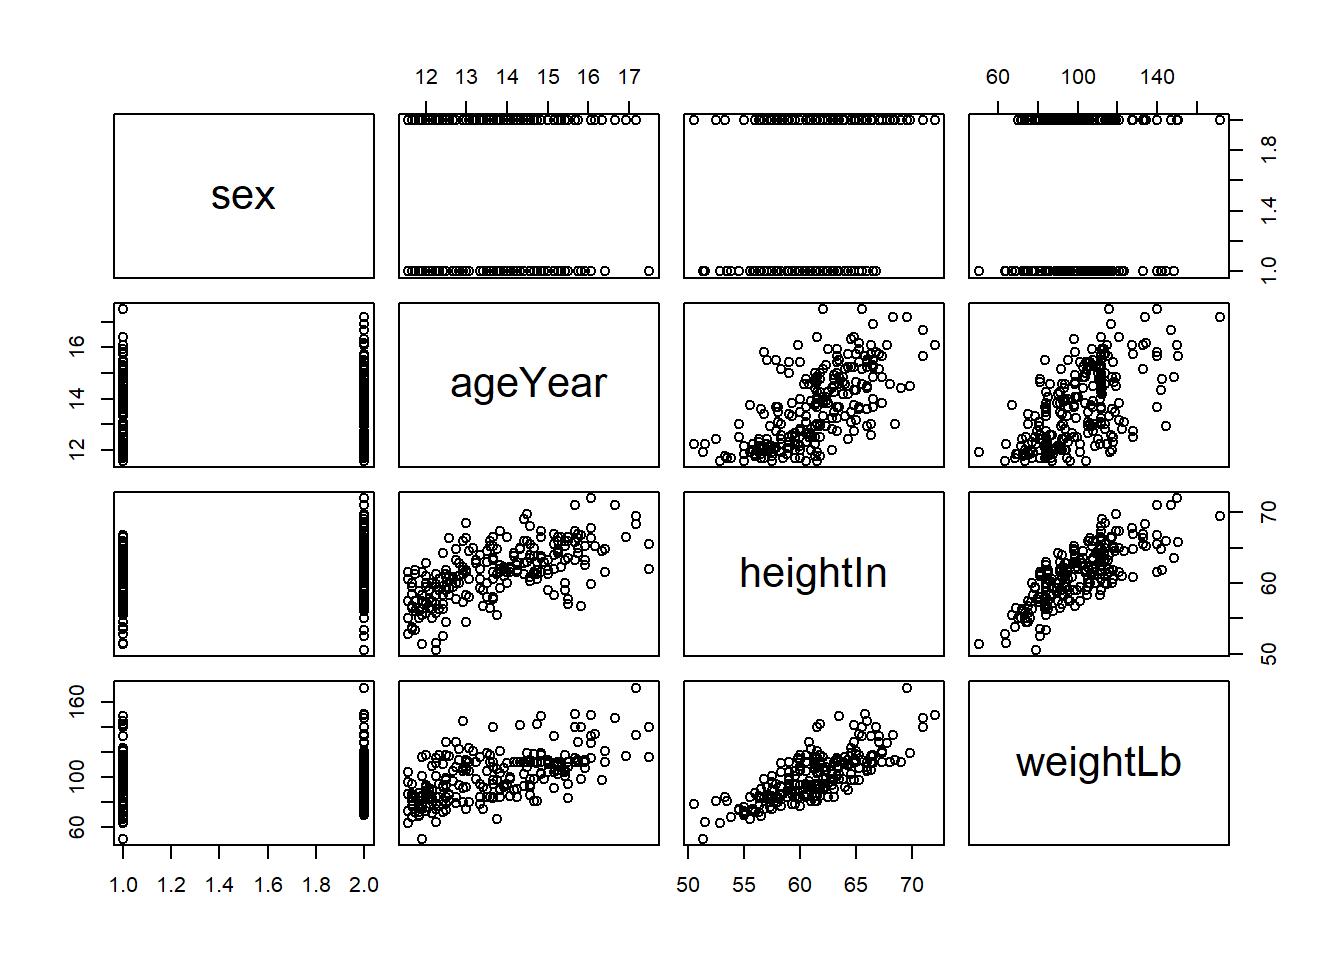
\includegraphics[keepaspectratio]{Scatterplots_files/figure-pdf/unnamed-chunk-13-1.pdf}}

Take a look at this matrix and you will see in the central diagonal
cells the names of the variables that we have in our dataset. This
diagonal acts as a sort of mirror for the visualisation. Since scatter
plots are inherently pairwise visualisations, we interpret each ``cell''
in this matrix, each plot as a pairwise depiction of the variables on
the diagonal.

For our purposes, let's name the rows in this matrix 1-4 (top to bottom)
and the columns A-D (left to right). In this plot cell 1A has the
variable sex. Cell 1B Therefore has the scatter plot of ageyear (in cell
B2) and sex (1A). Age is on the x axis while sex is on the y. Cell 2C,
then, shows the scatter plot between age and height (the one we have
been looking at so far). Finally, 3D shows the scatter plot of height
and weight. Following this logic, then What is represented in cell 1C?

Sex is on the y axis and height in on the x axis. The left side of this
matrix, ``under'' the diagonal, is just the reverse of what we have
discussed with the axes flipped.

Is this starting to make sense? Spend some time now to familiarise
yourself with this and describe with a partner the apparent association
between each of the pairs (don't worry about the sex variable).

\section{Activity}\label{activity}

From Winston Chang's \href{https://r-graphics.org/}{R Graphics
Cookbook}:

Select one or two and discuss their utility with a partner.

\subsection{5.3}\label{section-7}

\begin{itemize}
\tightlist
\item
  Alternative point shapes
\end{itemize}

\subsection{5.4}\label{section-8}

\begin{itemize}
\tightlist
\item
  You want to show even more in this plot. You Can plot another
  continuous variable to the colour or the size of the points.
\end{itemize}

\subsection{5.5}\label{section-9}

\begin{itemize}
\tightlist
\item
  What to do if you have a scatter plot with many overlapping points? -
  Note, this recipe uses a different dataset (diamonds).
\end{itemize}

\subsection{5.6}\label{section-10}

\begin{itemize}
\tightlist
\item
  You want to plot a regression line on a scatter plot but with a binary
  variable (0, 1).
\end{itemize}

\chapter{Beyond Static Visualisation}\label{beyond-static-visualisation}

\begin{Shaded}
\begin{Highlighting}[]
\FunctionTok{library}\NormalTok{(ggplot2)}
\FunctionTok{library}\NormalTok{(plotly)}
\FunctionTok{library}\NormalTok{(dplyr)}
\FunctionTok{library}\NormalTok{(gganimate)}
\end{Highlighting}
\end{Shaded}

\section{Interactive Plots}\label{interactive-plots}

So far, we have generated static and dynamic plots which make for some
nice visualisations. However, we may wish to make some interactive
visualisations. Interaction can be a useful tool in visualisation
because it gets people involved with the data directly. There are many
packages that can do this. The most basic serves as an extension of
ggplot2, is pltoly. Let's return to our paired down coffee scatter plot
and make this interactive.

\begin{Shaded}
\begin{Highlighting}[]
\NormalTok{coffee }\OtherTok{\textless{}{-}} \FunctionTok{read.csv}\NormalTok{(}\FunctionTok{file.choose}\NormalTok{())}

\NormalTok{coffee\_small }\OtherTok{\textless{}{-}}\NormalTok{ coffee }\SpecialCharTok{\%\textgreater{}\%}
  \FunctionTok{filter}\NormalTok{(Location.Country }\SpecialCharTok{==} \FunctionTok{c}\NormalTok{(}\StringTok{"Mexico"}\NormalTok{, }\StringTok{"Colombia"}\NormalTok{)) }\SpecialCharTok{\%\textgreater{}\%}
  \FunctionTok{select}\NormalTok{(Location.Country, Year, Data.Scores.Aroma, Data.Scores.Flavor)}
\end{Highlighting}
\end{Shaded}

No we can recreate the plot we generated showing the relationship
between aroma and flavour across two countries - Mexico and Colombia. To
make a plot interactive, simply setup your ggplot2 syntax, store it as
an object, then plot using ggplotly(). Now, hover over each point and
you will see that each observation has a label indicating the scores and
which location the are from. At the top of the plot window there are
some other options like zooming in and out, panning around, or
highlighting a section of the plot.

\begin{Shaded}
\begin{Highlighting}[]
\NormalTok{coff }\OtherTok{\textless{}{-}} \FunctionTok{ggplot}\NormalTok{(coffee\_small, }\FunctionTok{aes}\NormalTok{(}\AttributeTok{x =}\NormalTok{ Data.Scores.Aroma, }\AttributeTok{y =}\NormalTok{ Data.Scores.Flavor, }\AttributeTok{colour =}\NormalTok{ Location.Country)) }\SpecialCharTok{+}
  \FunctionTok{geom\_point}\NormalTok{() }
\FunctionTok{ggplotly}\NormalTok{(coff)}
\end{Highlighting}
\end{Shaded}

\pandocbounded{\includegraphics[keepaspectratio]{Beyond-Static-Visualisation_files/figure-pdf/unnamed-chunk-3-1.pdf}}

Desnity plots\ldots\ldots\ldots\ldots\ldots{}

\begin{Shaded}
\begin{Highlighting}[]
\NormalTok{cof\_dens }\OtherTok{\textless{}{-}} \FunctionTok{ggplot}\NormalTok{(coffee\_small, }\FunctionTok{aes}\NormalTok{(}\AttributeTok{x =}\NormalTok{ Data.Scores.Flavor, }\AttributeTok{colour =}\NormalTok{ Location.Country, }\AttributeTok{fill =}\NormalTok{ Location.Country)) }\SpecialCharTok{+}
\FunctionTok{geom\_density}\NormalTok{(}\AttributeTok{alpha =} \FloatTok{0.25}\NormalTok{) }

\FunctionTok{ggplotly}\NormalTok{(cof\_dens)}
\end{Highlighting}
\end{Shaded}

\pandocbounded{\includegraphics[keepaspectratio]{Beyond-Static-Visualisation_files/figure-pdf/unnamed-chunk-4-1.pdf}}

This provides an interactive way for your constituents to engage with
your data. Let's look at some other examples and explore their uses. The
syntax and logic is the same for boxplots. I think these are among the
most useful when interactive. Comparing two groups side-by-side is not
always very easy to do without a ruler to see where each element of the
distribution fits along the y-axis. However, when I however over the
boxes, I can see the numeric values and easily compare those across
groups.

\begin{Shaded}
\begin{Highlighting}[]
\NormalTok{cof\_box }\OtherTok{\textless{}{-}} \FunctionTok{ggplot}\NormalTok{(coffee\_small, }\FunctionTok{aes}\NormalTok{(}\AttributeTok{x =}\NormalTok{ Location.Country, }\AttributeTok{y =}\NormalTok{ Data.Scores.Flavor, }\AttributeTok{color =}\NormalTok{ Location.Country)) }\SpecialCharTok{+}
\FunctionTok{geom\_boxplot}\NormalTok{() }
  
\FunctionTok{ggplotly}\NormalTok{(cof\_box)  }
\end{Highlighting}
\end{Shaded}

\pandocbounded{\includegraphics[keepaspectratio]{Beyond-Static-Visualisation_files/figure-pdf/unnamed-chunk-5-1.pdf}}

\section{Dynamic Plots}\label{dynamic-plots}

You may need to make some dynamic plots that move with time or another
category. This vignette is designed to spark some of your imagination on
a few different types of plots. First, we are going to use the
`gganimate' package which is an extension of ggplot designed to create
dynamic plots.

The package gganimate will work with most plots. I encourage you to
think about the uses of having dynamic plots. Some plots make more sense
than others to make dynamic. For now, though, let's take a look at some
scatterplots. There are two main uses of dynamic scatter plots, say you
want to demonstrate the relationship between two variables over time, or
perhaps, across different groups. You can do so using gganimate's
transition\_time() and transition\_state() arguments.

We will be using the coffee dataset for these examples.

\begin{Shaded}
\begin{Highlighting}[]
\NormalTok{coffee }\OtherTok{\textless{}{-}} \FunctionTok{read.csv}\NormalTok{(}\FunctionTok{file.choose}\NormalTok{())}
\FunctionTok{colnames}\NormalTok{(coffee)}
\end{Highlighting}
\end{Shaded}

\begin{verbatim}
 [1] "Location.Country"               "Location.Region"               
 [3] "Location.Altitude.Min"          "Location.Altitude.Max"         
 [5] "Location.Altitude.Average"      "Year"                          
 [7] "Data.Owner"                     "Data.Type.Species"             
 [9] "Data.Type.Variety"              "Data.Type.Processing.method"   
[11] "Data.Production.Number.of.bags" "Data.Production.Bag.weight"    
[13] "Data.Scores.Aroma"              "Data.Scores.Flavor"            
[15] "Data.Scores.Aftertaste"         "Data.Scores.Acidity"           
[17] "Data.Scores.Body"               "Data.Scores.Balance"           
[19] "Data.Scores.Uniformity"         "Data.Scores.Sweetness"         
[21] "Data.Scores.Moisture"           "Data.Scores.Total"             
[23] "Data.Color"                    
\end{verbatim}

First, we will take a look at the relationship between flavour and
aroma.

\begin{Shaded}
\begin{Highlighting}[]
\FunctionTok{ggplot}\NormalTok{(coffee, }\FunctionTok{aes}\NormalTok{(}\AttributeTok{x =}\NormalTok{ Data.Scores.Aroma, }\AttributeTok{y =}\NormalTok{ Data.Scores.Flavor)) }\SpecialCharTok{+}
\FunctionTok{geom\_point}\NormalTok{() }
\end{Highlighting}
\end{Shaded}

\pandocbounded{\includegraphics[keepaspectratio]{Beyond-Static-Visualisation_files/figure-pdf/unnamed-chunk-7-1.pdf}}

There appears to be a linear relationship between these two variables.
As aroma increases, so too, does the flavour of the coffee. However, we
can tell more of a story here using the longitudinal nature of the data
and the locations from where the coffee is sourced.

Additionally, we may want to remove the single point from our visual. We
can do that by changing the limit the axes or removing that outlier. For
now, we will simply change the limits of the plot.

First, let's show this association over time by using the
transition\_time() argument associated with gganimate. We select the
`Year'' variable which is, in this dataset, the time indicator. We also
use the labs() option to add a title (the year) and the 'linear' option
for a smooth transition between years. Note, this plot might take a
short while to visualise.

\begin{Shaded}
\begin{Highlighting}[]
\FunctionTok{ggplot}\NormalTok{(coffee, }\FunctionTok{aes}\NormalTok{(}\AttributeTok{x =}\NormalTok{ Data.Scores.Aroma, }\AttributeTok{y =}\NormalTok{ Data.Scores.Flavor)) }\SpecialCharTok{+}
\FunctionTok{geom\_point}\NormalTok{() }\SpecialCharTok{+}
  \FunctionTok{xlim}\NormalTok{(}\FloatTok{6.5}\NormalTok{, }\ConstantTok{NA}\NormalTok{) }\SpecialCharTok{+}
  \FunctionTok{ylim}\NormalTok{(}\DecValTok{5}\NormalTok{, }\ConstantTok{NA}\NormalTok{)}\SpecialCharTok{+}  
  \FunctionTok{transition\_time}\NormalTok{(Year) }\SpecialCharTok{+}
  \FunctionTok{ease\_aes}\NormalTok{(}\StringTok{\textquotesingle{}linear\textquotesingle{}}\NormalTok{) }\SpecialCharTok{+} 
  \FunctionTok{labs}\NormalTok{(}\AttributeTok{title =} \StringTok{\textquotesingle{}Year: \{frame\_time\}\textquotesingle{}}\NormalTok{)}
\end{Highlighting}
\end{Shaded}

\pandocbounded{\includegraphics[keepaspectratio]{Beyond-Static-Visualisation_files/figure-pdf/unnamed-chunk-8-1.pdf}}

\pandocbounded{\includegraphics[keepaspectratio]{Beyond-Static-Visualisation_files/figure-pdf/unnamed-chunk-8-2.pdf}}

\pandocbounded{\includegraphics[keepaspectratio]{Beyond-Static-Visualisation_files/figure-pdf/unnamed-chunk-8-3.pdf}}

\pandocbounded{\includegraphics[keepaspectratio]{Beyond-Static-Visualisation_files/figure-pdf/unnamed-chunk-8-4.pdf}}

\pandocbounded{\includegraphics[keepaspectratio]{Beyond-Static-Visualisation_files/figure-pdf/unnamed-chunk-8-5.pdf}}

\pandocbounded{\includegraphics[keepaspectratio]{Beyond-Static-Visualisation_files/figure-pdf/unnamed-chunk-8-6.pdf}}

\pandocbounded{\includegraphics[keepaspectratio]{Beyond-Static-Visualisation_files/figure-pdf/unnamed-chunk-8-7.pdf}}

\pandocbounded{\includegraphics[keepaspectratio]{Beyond-Static-Visualisation_files/figure-pdf/unnamed-chunk-8-8.pdf}}

\pandocbounded{\includegraphics[keepaspectratio]{Beyond-Static-Visualisation_files/figure-pdf/unnamed-chunk-8-9.pdf}}

\pandocbounded{\includegraphics[keepaspectratio]{Beyond-Static-Visualisation_files/figure-pdf/unnamed-chunk-8-10.pdf}}

\pandocbounded{\includegraphics[keepaspectratio]{Beyond-Static-Visualisation_files/figure-pdf/unnamed-chunk-8-11.pdf}}

\pandocbounded{\includegraphics[keepaspectratio]{Beyond-Static-Visualisation_files/figure-pdf/unnamed-chunk-8-12.pdf}}

\pandocbounded{\includegraphics[keepaspectratio]{Beyond-Static-Visualisation_files/figure-pdf/unnamed-chunk-8-13.pdf}}

\pandocbounded{\includegraphics[keepaspectratio]{Beyond-Static-Visualisation_files/figure-pdf/unnamed-chunk-8-14.pdf}}

\pandocbounded{\includegraphics[keepaspectratio]{Beyond-Static-Visualisation_files/figure-pdf/unnamed-chunk-8-15.pdf}}

\pandocbounded{\includegraphics[keepaspectratio]{Beyond-Static-Visualisation_files/figure-pdf/unnamed-chunk-8-16.pdf}}

\pandocbounded{\includegraphics[keepaspectratio]{Beyond-Static-Visualisation_files/figure-pdf/unnamed-chunk-8-17.pdf}}

\pandocbounded{\includegraphics[keepaspectratio]{Beyond-Static-Visualisation_files/figure-pdf/unnamed-chunk-8-18.pdf}}

\pandocbounded{\includegraphics[keepaspectratio]{Beyond-Static-Visualisation_files/figure-pdf/unnamed-chunk-8-19.pdf}}

\pandocbounded{\includegraphics[keepaspectratio]{Beyond-Static-Visualisation_files/figure-pdf/unnamed-chunk-8-20.pdf}}

\pandocbounded{\includegraphics[keepaspectratio]{Beyond-Static-Visualisation_files/figure-pdf/unnamed-chunk-8-21.pdf}}

\pandocbounded{\includegraphics[keepaspectratio]{Beyond-Static-Visualisation_files/figure-pdf/unnamed-chunk-8-22.pdf}}

\pandocbounded{\includegraphics[keepaspectratio]{Beyond-Static-Visualisation_files/figure-pdf/unnamed-chunk-8-23.pdf}}

\pandocbounded{\includegraphics[keepaspectratio]{Beyond-Static-Visualisation_files/figure-pdf/unnamed-chunk-8-24.pdf}}

\pandocbounded{\includegraphics[keepaspectratio]{Beyond-Static-Visualisation_files/figure-pdf/unnamed-chunk-8-25.pdf}}

\pandocbounded{\includegraphics[keepaspectratio]{Beyond-Static-Visualisation_files/figure-pdf/unnamed-chunk-8-26.pdf}}

\pandocbounded{\includegraphics[keepaspectratio]{Beyond-Static-Visualisation_files/figure-pdf/unnamed-chunk-8-27.pdf}}

\pandocbounded{\includegraphics[keepaspectratio]{Beyond-Static-Visualisation_files/figure-pdf/unnamed-chunk-8-28.pdf}}

\pandocbounded{\includegraphics[keepaspectratio]{Beyond-Static-Visualisation_files/figure-pdf/unnamed-chunk-8-29.pdf}}

\pandocbounded{\includegraphics[keepaspectratio]{Beyond-Static-Visualisation_files/figure-pdf/unnamed-chunk-8-30.pdf}}

\pandocbounded{\includegraphics[keepaspectratio]{Beyond-Static-Visualisation_files/figure-pdf/unnamed-chunk-8-31.pdf}}

\pandocbounded{\includegraphics[keepaspectratio]{Beyond-Static-Visualisation_files/figure-pdf/unnamed-chunk-8-32.pdf}}

\pandocbounded{\includegraphics[keepaspectratio]{Beyond-Static-Visualisation_files/figure-pdf/unnamed-chunk-8-33.pdf}}

\pandocbounded{\includegraphics[keepaspectratio]{Beyond-Static-Visualisation_files/figure-pdf/unnamed-chunk-8-34.pdf}}

\pandocbounded{\includegraphics[keepaspectratio]{Beyond-Static-Visualisation_files/figure-pdf/unnamed-chunk-8-35.pdf}}

\pandocbounded{\includegraphics[keepaspectratio]{Beyond-Static-Visualisation_files/figure-pdf/unnamed-chunk-8-36.pdf}}

\pandocbounded{\includegraphics[keepaspectratio]{Beyond-Static-Visualisation_files/figure-pdf/unnamed-chunk-8-37.pdf}}

\pandocbounded{\includegraphics[keepaspectratio]{Beyond-Static-Visualisation_files/figure-pdf/unnamed-chunk-8-38.pdf}}

\pandocbounded{\includegraphics[keepaspectratio]{Beyond-Static-Visualisation_files/figure-pdf/unnamed-chunk-8-39.pdf}}

\pandocbounded{\includegraphics[keepaspectratio]{Beyond-Static-Visualisation_files/figure-pdf/unnamed-chunk-8-40.pdf}}

\pandocbounded{\includegraphics[keepaspectratio]{Beyond-Static-Visualisation_files/figure-pdf/unnamed-chunk-8-41.pdf}}

\pandocbounded{\includegraphics[keepaspectratio]{Beyond-Static-Visualisation_files/figure-pdf/unnamed-chunk-8-42.pdf}}

\pandocbounded{\includegraphics[keepaspectratio]{Beyond-Static-Visualisation_files/figure-pdf/unnamed-chunk-8-43.pdf}}

\pandocbounded{\includegraphics[keepaspectratio]{Beyond-Static-Visualisation_files/figure-pdf/unnamed-chunk-8-44.pdf}}

\pandocbounded{\includegraphics[keepaspectratio]{Beyond-Static-Visualisation_files/figure-pdf/unnamed-chunk-8-45.pdf}}

\pandocbounded{\includegraphics[keepaspectratio]{Beyond-Static-Visualisation_files/figure-pdf/unnamed-chunk-8-46.pdf}}

\pandocbounded{\includegraphics[keepaspectratio]{Beyond-Static-Visualisation_files/figure-pdf/unnamed-chunk-8-47.pdf}}

\pandocbounded{\includegraphics[keepaspectratio]{Beyond-Static-Visualisation_files/figure-pdf/unnamed-chunk-8-48.pdf}}

\pandocbounded{\includegraphics[keepaspectratio]{Beyond-Static-Visualisation_files/figure-pdf/unnamed-chunk-8-49.pdf}}

\pandocbounded{\includegraphics[keepaspectratio]{Beyond-Static-Visualisation_files/figure-pdf/unnamed-chunk-8-50.pdf}}

\pandocbounded{\includegraphics[keepaspectratio]{Beyond-Static-Visualisation_files/figure-pdf/unnamed-chunk-8-51.pdf}}

\pandocbounded{\includegraphics[keepaspectratio]{Beyond-Static-Visualisation_files/figure-pdf/unnamed-chunk-8-52.pdf}}

\pandocbounded{\includegraphics[keepaspectratio]{Beyond-Static-Visualisation_files/figure-pdf/unnamed-chunk-8-53.pdf}}

\pandocbounded{\includegraphics[keepaspectratio]{Beyond-Static-Visualisation_files/figure-pdf/unnamed-chunk-8-54.pdf}}

\pandocbounded{\includegraphics[keepaspectratio]{Beyond-Static-Visualisation_files/figure-pdf/unnamed-chunk-8-55.pdf}}

\pandocbounded{\includegraphics[keepaspectratio]{Beyond-Static-Visualisation_files/figure-pdf/unnamed-chunk-8-56.pdf}}

\pandocbounded{\includegraphics[keepaspectratio]{Beyond-Static-Visualisation_files/figure-pdf/unnamed-chunk-8-57.pdf}}

\pandocbounded{\includegraphics[keepaspectratio]{Beyond-Static-Visualisation_files/figure-pdf/unnamed-chunk-8-58.pdf}}

\pandocbounded{\includegraphics[keepaspectratio]{Beyond-Static-Visualisation_files/figure-pdf/unnamed-chunk-8-59.pdf}}

\pandocbounded{\includegraphics[keepaspectratio]{Beyond-Static-Visualisation_files/figure-pdf/unnamed-chunk-8-60.pdf}}

\pandocbounded{\includegraphics[keepaspectratio]{Beyond-Static-Visualisation_files/figure-pdf/unnamed-chunk-8-61.pdf}}

\pandocbounded{\includegraphics[keepaspectratio]{Beyond-Static-Visualisation_files/figure-pdf/unnamed-chunk-8-62.pdf}}

\pandocbounded{\includegraphics[keepaspectratio]{Beyond-Static-Visualisation_files/figure-pdf/unnamed-chunk-8-63.pdf}}

\pandocbounded{\includegraphics[keepaspectratio]{Beyond-Static-Visualisation_files/figure-pdf/unnamed-chunk-8-64.pdf}}

\pandocbounded{\includegraphics[keepaspectratio]{Beyond-Static-Visualisation_files/figure-pdf/unnamed-chunk-8-65.pdf}}

\pandocbounded{\includegraphics[keepaspectratio]{Beyond-Static-Visualisation_files/figure-pdf/unnamed-chunk-8-66.pdf}}

\pandocbounded{\includegraphics[keepaspectratio]{Beyond-Static-Visualisation_files/figure-pdf/unnamed-chunk-8-67.pdf}}

\pandocbounded{\includegraphics[keepaspectratio]{Beyond-Static-Visualisation_files/figure-pdf/unnamed-chunk-8-68.pdf}}

\pandocbounded{\includegraphics[keepaspectratio]{Beyond-Static-Visualisation_files/figure-pdf/unnamed-chunk-8-69.pdf}}

\pandocbounded{\includegraphics[keepaspectratio]{Beyond-Static-Visualisation_files/figure-pdf/unnamed-chunk-8-70.pdf}}

\pandocbounded{\includegraphics[keepaspectratio]{Beyond-Static-Visualisation_files/figure-pdf/unnamed-chunk-8-71.pdf}}

\pandocbounded{\includegraphics[keepaspectratio]{Beyond-Static-Visualisation_files/figure-pdf/unnamed-chunk-8-72.pdf}}

\pandocbounded{\includegraphics[keepaspectratio]{Beyond-Static-Visualisation_files/figure-pdf/unnamed-chunk-8-73.pdf}}

\pandocbounded{\includegraphics[keepaspectratio]{Beyond-Static-Visualisation_files/figure-pdf/unnamed-chunk-8-74.pdf}}

\pandocbounded{\includegraphics[keepaspectratio]{Beyond-Static-Visualisation_files/figure-pdf/unnamed-chunk-8-75.pdf}}

\pandocbounded{\includegraphics[keepaspectratio]{Beyond-Static-Visualisation_files/figure-pdf/unnamed-chunk-8-76.pdf}}

\pandocbounded{\includegraphics[keepaspectratio]{Beyond-Static-Visualisation_files/figure-pdf/unnamed-chunk-8-77.pdf}}

\pandocbounded{\includegraphics[keepaspectratio]{Beyond-Static-Visualisation_files/figure-pdf/unnamed-chunk-8-78.pdf}}

\pandocbounded{\includegraphics[keepaspectratio]{Beyond-Static-Visualisation_files/figure-pdf/unnamed-chunk-8-79.pdf}}

\pandocbounded{\includegraphics[keepaspectratio]{Beyond-Static-Visualisation_files/figure-pdf/unnamed-chunk-8-80.pdf}}

\pandocbounded{\includegraphics[keepaspectratio]{Beyond-Static-Visualisation_files/figure-pdf/unnamed-chunk-8-81.pdf}}

\pandocbounded{\includegraphics[keepaspectratio]{Beyond-Static-Visualisation_files/figure-pdf/unnamed-chunk-8-82.pdf}}

\pandocbounded{\includegraphics[keepaspectratio]{Beyond-Static-Visualisation_files/figure-pdf/unnamed-chunk-8-83.pdf}}

\pandocbounded{\includegraphics[keepaspectratio]{Beyond-Static-Visualisation_files/figure-pdf/unnamed-chunk-8-84.pdf}}

\pandocbounded{\includegraphics[keepaspectratio]{Beyond-Static-Visualisation_files/figure-pdf/unnamed-chunk-8-85.pdf}}

\pandocbounded{\includegraphics[keepaspectratio]{Beyond-Static-Visualisation_files/figure-pdf/unnamed-chunk-8-86.pdf}}

\pandocbounded{\includegraphics[keepaspectratio]{Beyond-Static-Visualisation_files/figure-pdf/unnamed-chunk-8-87.pdf}}

\pandocbounded{\includegraphics[keepaspectratio]{Beyond-Static-Visualisation_files/figure-pdf/unnamed-chunk-8-88.pdf}}

\pandocbounded{\includegraphics[keepaspectratio]{Beyond-Static-Visualisation_files/figure-pdf/unnamed-chunk-8-89.pdf}}

\pandocbounded{\includegraphics[keepaspectratio]{Beyond-Static-Visualisation_files/figure-pdf/unnamed-chunk-8-90.pdf}}

\pandocbounded{\includegraphics[keepaspectratio]{Beyond-Static-Visualisation_files/figure-pdf/unnamed-chunk-8-91.pdf}}

\pandocbounded{\includegraphics[keepaspectratio]{Beyond-Static-Visualisation_files/figure-pdf/unnamed-chunk-8-92.pdf}}

\pandocbounded{\includegraphics[keepaspectratio]{Beyond-Static-Visualisation_files/figure-pdf/unnamed-chunk-8-93.pdf}}

\pandocbounded{\includegraphics[keepaspectratio]{Beyond-Static-Visualisation_files/figure-pdf/unnamed-chunk-8-94.pdf}}

\pandocbounded{\includegraphics[keepaspectratio]{Beyond-Static-Visualisation_files/figure-pdf/unnamed-chunk-8-95.pdf}}

\pandocbounded{\includegraphics[keepaspectratio]{Beyond-Static-Visualisation_files/figure-pdf/unnamed-chunk-8-96.pdf}}

\pandocbounded{\includegraphics[keepaspectratio]{Beyond-Static-Visualisation_files/figure-pdf/unnamed-chunk-8-97.pdf}}

\pandocbounded{\includegraphics[keepaspectratio]{Beyond-Static-Visualisation_files/figure-pdf/unnamed-chunk-8-98.pdf}}

\pandocbounded{\includegraphics[keepaspectratio]{Beyond-Static-Visualisation_files/figure-pdf/unnamed-chunk-8-99.pdf}}

\pandocbounded{\includegraphics[keepaspectratio]{Beyond-Static-Visualisation_files/figure-pdf/unnamed-chunk-8-100.pdf}}

What does this plot tell you?

Next, we may wish to demonstrate if the observed relationship between
aroma and flavour is the same across locations. We have an indicator
showing which country from which the coffee is sourced. Here, then, we
don't have a `time' variable, but our third variable of interest is the
location. This is a categorical variable indicating which country the
coffee is sourced from. Thus, we use the transition\_states() argument
and set it to the `Location.Country' variable. This provides a scatter
plot that rotates through the points of each location.

\begin{Shaded}
\begin{Highlighting}[]
\FunctionTok{ggplot}\NormalTok{(coffee, }\FunctionTok{aes}\NormalTok{(}\AttributeTok{x =}\NormalTok{ Data.Scores.Aroma, }\AttributeTok{y =}\NormalTok{ Data.Scores.Flavor)) }\SpecialCharTok{+}
\FunctionTok{geom\_point}\NormalTok{() }\SpecialCharTok{+}
  \FunctionTok{xlim}\NormalTok{(}\FloatTok{6.5}\NormalTok{, }\ConstantTok{NA}\NormalTok{) }\SpecialCharTok{+}
  \FunctionTok{ylim}\NormalTok{(}\DecValTok{5}\NormalTok{, }\ConstantTok{NA}\NormalTok{)}\SpecialCharTok{+}  
  \FunctionTok{transition\_states}\NormalTok{(Location.Country) }\SpecialCharTok{+}
  \FunctionTok{ease\_aes}\NormalTok{(}\StringTok{\textquotesingle{}linear\textquotesingle{}}\NormalTok{) }\SpecialCharTok{+}
  \FunctionTok{labs}\NormalTok{(}\AttributeTok{title =} \StringTok{\textquotesingle{}Country: \{closest\_state\}\textquotesingle{}}\NormalTok{)}
\end{Highlighting}
\end{Shaded}

\pandocbounded{\includegraphics[keepaspectratio]{Beyond-Static-Visualisation_files/figure-pdf/unnamed-chunk-9-1.pdf}}

\pandocbounded{\includegraphics[keepaspectratio]{Beyond-Static-Visualisation_files/figure-pdf/unnamed-chunk-9-2.pdf}}

\pandocbounded{\includegraphics[keepaspectratio]{Beyond-Static-Visualisation_files/figure-pdf/unnamed-chunk-9-3.pdf}}

\pandocbounded{\includegraphics[keepaspectratio]{Beyond-Static-Visualisation_files/figure-pdf/unnamed-chunk-9-4.pdf}}

\pandocbounded{\includegraphics[keepaspectratio]{Beyond-Static-Visualisation_files/figure-pdf/unnamed-chunk-9-5.pdf}}

\pandocbounded{\includegraphics[keepaspectratio]{Beyond-Static-Visualisation_files/figure-pdf/unnamed-chunk-9-6.pdf}}

\pandocbounded{\includegraphics[keepaspectratio]{Beyond-Static-Visualisation_files/figure-pdf/unnamed-chunk-9-7.pdf}}

\pandocbounded{\includegraphics[keepaspectratio]{Beyond-Static-Visualisation_files/figure-pdf/unnamed-chunk-9-8.pdf}}

\pandocbounded{\includegraphics[keepaspectratio]{Beyond-Static-Visualisation_files/figure-pdf/unnamed-chunk-9-9.pdf}}

\pandocbounded{\includegraphics[keepaspectratio]{Beyond-Static-Visualisation_files/figure-pdf/unnamed-chunk-9-10.pdf}}

\pandocbounded{\includegraphics[keepaspectratio]{Beyond-Static-Visualisation_files/figure-pdf/unnamed-chunk-9-11.pdf}}

\pandocbounded{\includegraphics[keepaspectratio]{Beyond-Static-Visualisation_files/figure-pdf/unnamed-chunk-9-12.pdf}}

\pandocbounded{\includegraphics[keepaspectratio]{Beyond-Static-Visualisation_files/figure-pdf/unnamed-chunk-9-13.pdf}}

\pandocbounded{\includegraphics[keepaspectratio]{Beyond-Static-Visualisation_files/figure-pdf/unnamed-chunk-9-14.pdf}}

\pandocbounded{\includegraphics[keepaspectratio]{Beyond-Static-Visualisation_files/figure-pdf/unnamed-chunk-9-15.pdf}}

\pandocbounded{\includegraphics[keepaspectratio]{Beyond-Static-Visualisation_files/figure-pdf/unnamed-chunk-9-16.pdf}}

\pandocbounded{\includegraphics[keepaspectratio]{Beyond-Static-Visualisation_files/figure-pdf/unnamed-chunk-9-17.pdf}}

\pandocbounded{\includegraphics[keepaspectratio]{Beyond-Static-Visualisation_files/figure-pdf/unnamed-chunk-9-18.pdf}}

\pandocbounded{\includegraphics[keepaspectratio]{Beyond-Static-Visualisation_files/figure-pdf/unnamed-chunk-9-19.pdf}}

\pandocbounded{\includegraphics[keepaspectratio]{Beyond-Static-Visualisation_files/figure-pdf/unnamed-chunk-9-20.pdf}}

\pandocbounded{\includegraphics[keepaspectratio]{Beyond-Static-Visualisation_files/figure-pdf/unnamed-chunk-9-21.pdf}}

\pandocbounded{\includegraphics[keepaspectratio]{Beyond-Static-Visualisation_files/figure-pdf/unnamed-chunk-9-22.pdf}}

\pandocbounded{\includegraphics[keepaspectratio]{Beyond-Static-Visualisation_files/figure-pdf/unnamed-chunk-9-23.pdf}}

\pandocbounded{\includegraphics[keepaspectratio]{Beyond-Static-Visualisation_files/figure-pdf/unnamed-chunk-9-24.pdf}}

\pandocbounded{\includegraphics[keepaspectratio]{Beyond-Static-Visualisation_files/figure-pdf/unnamed-chunk-9-25.pdf}}

\pandocbounded{\includegraphics[keepaspectratio]{Beyond-Static-Visualisation_files/figure-pdf/unnamed-chunk-9-26.pdf}}

\pandocbounded{\includegraphics[keepaspectratio]{Beyond-Static-Visualisation_files/figure-pdf/unnamed-chunk-9-27.pdf}}

\pandocbounded{\includegraphics[keepaspectratio]{Beyond-Static-Visualisation_files/figure-pdf/unnamed-chunk-9-28.pdf}}

\pandocbounded{\includegraphics[keepaspectratio]{Beyond-Static-Visualisation_files/figure-pdf/unnamed-chunk-9-29.pdf}}

\pandocbounded{\includegraphics[keepaspectratio]{Beyond-Static-Visualisation_files/figure-pdf/unnamed-chunk-9-30.pdf}}

\pandocbounded{\includegraphics[keepaspectratio]{Beyond-Static-Visualisation_files/figure-pdf/unnamed-chunk-9-31.pdf}}

\pandocbounded{\includegraphics[keepaspectratio]{Beyond-Static-Visualisation_files/figure-pdf/unnamed-chunk-9-32.pdf}}

\pandocbounded{\includegraphics[keepaspectratio]{Beyond-Static-Visualisation_files/figure-pdf/unnamed-chunk-9-33.pdf}}

\pandocbounded{\includegraphics[keepaspectratio]{Beyond-Static-Visualisation_files/figure-pdf/unnamed-chunk-9-34.pdf}}

\pandocbounded{\includegraphics[keepaspectratio]{Beyond-Static-Visualisation_files/figure-pdf/unnamed-chunk-9-35.pdf}}

\pandocbounded{\includegraphics[keepaspectratio]{Beyond-Static-Visualisation_files/figure-pdf/unnamed-chunk-9-36.pdf}}

\pandocbounded{\includegraphics[keepaspectratio]{Beyond-Static-Visualisation_files/figure-pdf/unnamed-chunk-9-37.pdf}}

\pandocbounded{\includegraphics[keepaspectratio]{Beyond-Static-Visualisation_files/figure-pdf/unnamed-chunk-9-38.pdf}}

\pandocbounded{\includegraphics[keepaspectratio]{Beyond-Static-Visualisation_files/figure-pdf/unnamed-chunk-9-39.pdf}}

\pandocbounded{\includegraphics[keepaspectratio]{Beyond-Static-Visualisation_files/figure-pdf/unnamed-chunk-9-40.pdf}}

\pandocbounded{\includegraphics[keepaspectratio]{Beyond-Static-Visualisation_files/figure-pdf/unnamed-chunk-9-41.pdf}}

\pandocbounded{\includegraphics[keepaspectratio]{Beyond-Static-Visualisation_files/figure-pdf/unnamed-chunk-9-42.pdf}}

\pandocbounded{\includegraphics[keepaspectratio]{Beyond-Static-Visualisation_files/figure-pdf/unnamed-chunk-9-43.pdf}}

\pandocbounded{\includegraphics[keepaspectratio]{Beyond-Static-Visualisation_files/figure-pdf/unnamed-chunk-9-44.pdf}}

\pandocbounded{\includegraphics[keepaspectratio]{Beyond-Static-Visualisation_files/figure-pdf/unnamed-chunk-9-45.pdf}}

\pandocbounded{\includegraphics[keepaspectratio]{Beyond-Static-Visualisation_files/figure-pdf/unnamed-chunk-9-46.pdf}}

\pandocbounded{\includegraphics[keepaspectratio]{Beyond-Static-Visualisation_files/figure-pdf/unnamed-chunk-9-47.pdf}}

\pandocbounded{\includegraphics[keepaspectratio]{Beyond-Static-Visualisation_files/figure-pdf/unnamed-chunk-9-48.pdf}}

\pandocbounded{\includegraphics[keepaspectratio]{Beyond-Static-Visualisation_files/figure-pdf/unnamed-chunk-9-49.pdf}}

\pandocbounded{\includegraphics[keepaspectratio]{Beyond-Static-Visualisation_files/figure-pdf/unnamed-chunk-9-50.pdf}}

\pandocbounded{\includegraphics[keepaspectratio]{Beyond-Static-Visualisation_files/figure-pdf/unnamed-chunk-9-51.pdf}}

\pandocbounded{\includegraphics[keepaspectratio]{Beyond-Static-Visualisation_files/figure-pdf/unnamed-chunk-9-52.pdf}}

\pandocbounded{\includegraphics[keepaspectratio]{Beyond-Static-Visualisation_files/figure-pdf/unnamed-chunk-9-53.pdf}}

\pandocbounded{\includegraphics[keepaspectratio]{Beyond-Static-Visualisation_files/figure-pdf/unnamed-chunk-9-54.pdf}}

\pandocbounded{\includegraphics[keepaspectratio]{Beyond-Static-Visualisation_files/figure-pdf/unnamed-chunk-9-55.pdf}}

\pandocbounded{\includegraphics[keepaspectratio]{Beyond-Static-Visualisation_files/figure-pdf/unnamed-chunk-9-56.pdf}}

\pandocbounded{\includegraphics[keepaspectratio]{Beyond-Static-Visualisation_files/figure-pdf/unnamed-chunk-9-57.pdf}}

\pandocbounded{\includegraphics[keepaspectratio]{Beyond-Static-Visualisation_files/figure-pdf/unnamed-chunk-9-58.pdf}}

\pandocbounded{\includegraphics[keepaspectratio]{Beyond-Static-Visualisation_files/figure-pdf/unnamed-chunk-9-59.pdf}}

\pandocbounded{\includegraphics[keepaspectratio]{Beyond-Static-Visualisation_files/figure-pdf/unnamed-chunk-9-60.pdf}}

\pandocbounded{\includegraphics[keepaspectratio]{Beyond-Static-Visualisation_files/figure-pdf/unnamed-chunk-9-61.pdf}}

\pandocbounded{\includegraphics[keepaspectratio]{Beyond-Static-Visualisation_files/figure-pdf/unnamed-chunk-9-62.pdf}}

\pandocbounded{\includegraphics[keepaspectratio]{Beyond-Static-Visualisation_files/figure-pdf/unnamed-chunk-9-63.pdf}}

\pandocbounded{\includegraphics[keepaspectratio]{Beyond-Static-Visualisation_files/figure-pdf/unnamed-chunk-9-64.pdf}}

\pandocbounded{\includegraphics[keepaspectratio]{Beyond-Static-Visualisation_files/figure-pdf/unnamed-chunk-9-65.pdf}}

\pandocbounded{\includegraphics[keepaspectratio]{Beyond-Static-Visualisation_files/figure-pdf/unnamed-chunk-9-66.pdf}}

\pandocbounded{\includegraphics[keepaspectratio]{Beyond-Static-Visualisation_files/figure-pdf/unnamed-chunk-9-67.pdf}}

\pandocbounded{\includegraphics[keepaspectratio]{Beyond-Static-Visualisation_files/figure-pdf/unnamed-chunk-9-68.pdf}}

\pandocbounded{\includegraphics[keepaspectratio]{Beyond-Static-Visualisation_files/figure-pdf/unnamed-chunk-9-69.pdf}}

\pandocbounded{\includegraphics[keepaspectratio]{Beyond-Static-Visualisation_files/figure-pdf/unnamed-chunk-9-70.pdf}}

\pandocbounded{\includegraphics[keepaspectratio]{Beyond-Static-Visualisation_files/figure-pdf/unnamed-chunk-9-71.pdf}}

\pandocbounded{\includegraphics[keepaspectratio]{Beyond-Static-Visualisation_files/figure-pdf/unnamed-chunk-9-72.pdf}}

\pandocbounded{\includegraphics[keepaspectratio]{Beyond-Static-Visualisation_files/figure-pdf/unnamed-chunk-9-73.pdf}}

\pandocbounded{\includegraphics[keepaspectratio]{Beyond-Static-Visualisation_files/figure-pdf/unnamed-chunk-9-74.pdf}}

\pandocbounded{\includegraphics[keepaspectratio]{Beyond-Static-Visualisation_files/figure-pdf/unnamed-chunk-9-75.pdf}}

\pandocbounded{\includegraphics[keepaspectratio]{Beyond-Static-Visualisation_files/figure-pdf/unnamed-chunk-9-76.pdf}}

\pandocbounded{\includegraphics[keepaspectratio]{Beyond-Static-Visualisation_files/figure-pdf/unnamed-chunk-9-77.pdf}}

\pandocbounded{\includegraphics[keepaspectratio]{Beyond-Static-Visualisation_files/figure-pdf/unnamed-chunk-9-78.pdf}}

\pandocbounded{\includegraphics[keepaspectratio]{Beyond-Static-Visualisation_files/figure-pdf/unnamed-chunk-9-79.pdf}}

\pandocbounded{\includegraphics[keepaspectratio]{Beyond-Static-Visualisation_files/figure-pdf/unnamed-chunk-9-80.pdf}}

\pandocbounded{\includegraphics[keepaspectratio]{Beyond-Static-Visualisation_files/figure-pdf/unnamed-chunk-9-81.pdf}}

\pandocbounded{\includegraphics[keepaspectratio]{Beyond-Static-Visualisation_files/figure-pdf/unnamed-chunk-9-82.pdf}}

\pandocbounded{\includegraphics[keepaspectratio]{Beyond-Static-Visualisation_files/figure-pdf/unnamed-chunk-9-83.pdf}}

\pandocbounded{\includegraphics[keepaspectratio]{Beyond-Static-Visualisation_files/figure-pdf/unnamed-chunk-9-84.pdf}}

\pandocbounded{\includegraphics[keepaspectratio]{Beyond-Static-Visualisation_files/figure-pdf/unnamed-chunk-9-85.pdf}}

\pandocbounded{\includegraphics[keepaspectratio]{Beyond-Static-Visualisation_files/figure-pdf/unnamed-chunk-9-86.pdf}}

\pandocbounded{\includegraphics[keepaspectratio]{Beyond-Static-Visualisation_files/figure-pdf/unnamed-chunk-9-87.pdf}}

\pandocbounded{\includegraphics[keepaspectratio]{Beyond-Static-Visualisation_files/figure-pdf/unnamed-chunk-9-88.pdf}}

\pandocbounded{\includegraphics[keepaspectratio]{Beyond-Static-Visualisation_files/figure-pdf/unnamed-chunk-9-89.pdf}}

\pandocbounded{\includegraphics[keepaspectratio]{Beyond-Static-Visualisation_files/figure-pdf/unnamed-chunk-9-90.pdf}}

\pandocbounded{\includegraphics[keepaspectratio]{Beyond-Static-Visualisation_files/figure-pdf/unnamed-chunk-9-91.pdf}}

\pandocbounded{\includegraphics[keepaspectratio]{Beyond-Static-Visualisation_files/figure-pdf/unnamed-chunk-9-92.pdf}}

\pandocbounded{\includegraphics[keepaspectratio]{Beyond-Static-Visualisation_files/figure-pdf/unnamed-chunk-9-93.pdf}}

\pandocbounded{\includegraphics[keepaspectratio]{Beyond-Static-Visualisation_files/figure-pdf/unnamed-chunk-9-94.pdf}}

\pandocbounded{\includegraphics[keepaspectratio]{Beyond-Static-Visualisation_files/figure-pdf/unnamed-chunk-9-95.pdf}}

\pandocbounded{\includegraphics[keepaspectratio]{Beyond-Static-Visualisation_files/figure-pdf/unnamed-chunk-9-96.pdf}}

\pandocbounded{\includegraphics[keepaspectratio]{Beyond-Static-Visualisation_files/figure-pdf/unnamed-chunk-9-97.pdf}}

\pandocbounded{\includegraphics[keepaspectratio]{Beyond-Static-Visualisation_files/figure-pdf/unnamed-chunk-9-98.pdf}}

\pandocbounded{\includegraphics[keepaspectratio]{Beyond-Static-Visualisation_files/figure-pdf/unnamed-chunk-9-99.pdf}}

\pandocbounded{\includegraphics[keepaspectratio]{Beyond-Static-Visualisation_files/figure-pdf/unnamed-chunk-9-100.pdf}}

In order to save these use the anim\_save() function and save them as a
.gif so you can put it on a poster or website.

\begin{Shaded}
\begin{Highlighting}[]
\FunctionTok{anim\_save}\NormalTok{(}\StringTok{"Flavour\_Aroma\_Locations.gif"}\NormalTok{)}
\end{Highlighting}
\end{Shaded}

You may wish to combine some skills here. You may want to show the
relationship over time across these locations. To do so, you can use the
facet() option you have used before!

In this dataset, we have a lot of locations and so many facet windows -
probably too many to visualise properly. So, I create a small subset of
this dataset to pull a few locations and keep these focal variables.

\begin{Shaded}
\begin{Highlighting}[]
\NormalTok{coffee\_small }\OtherTok{\textless{}{-}}\NormalTok{ coffee }\SpecialCharTok{\%\textgreater{}\%}
  \FunctionTok{filter}\NormalTok{(Location.Country }\SpecialCharTok{==} \FunctionTok{c}\NormalTok{(}\StringTok{"Mexico"}\NormalTok{, }\StringTok{"Colombia"}\NormalTok{)) }\SpecialCharTok{\%\textgreater{}\%}
  \FunctionTok{select}\NormalTok{(Location.Country, Year, Data.Scores.Aroma, Data.Scores.Flavor)}
\end{Highlighting}
\end{Shaded}

Now we can create our plot!

\begin{Shaded}
\begin{Highlighting}[]
\FunctionTok{ggplot}\NormalTok{(coffee\_small, }\FunctionTok{aes}\NormalTok{(}\AttributeTok{x =}\NormalTok{ Data.Scores.Aroma, }\AttributeTok{y =}\NormalTok{ Data.Scores.Flavor)) }\SpecialCharTok{+}
\FunctionTok{geom\_point}\NormalTok{() }\SpecialCharTok{+}
  \FunctionTok{xlim}\NormalTok{(}\FloatTok{6.5}\NormalTok{, }\ConstantTok{NA}\NormalTok{) }\SpecialCharTok{+}
  \FunctionTok{ylim}\NormalTok{(}\DecValTok{5}\NormalTok{, }\ConstantTok{NA}\NormalTok{)}\SpecialCharTok{+}  
  \FunctionTok{facet\_grid}\NormalTok{(}\SpecialCharTok{\textasciitilde{}}\NormalTok{Location.Country) }\SpecialCharTok{+}
  \FunctionTok{transition\_time}\NormalTok{(Year) }\SpecialCharTok{+}
  \FunctionTok{ease\_aes}\NormalTok{(}\StringTok{\textquotesingle{}linear\textquotesingle{}}\NormalTok{) }\SpecialCharTok{+} 
  \FunctionTok{labs}\NormalTok{(}\AttributeTok{title =} \StringTok{\textquotesingle{}Year: \{frame\_time\}\textquotesingle{}}\NormalTok{) }
\end{Highlighting}
\end{Shaded}

\pandocbounded{\includegraphics[keepaspectratio]{Beyond-Static-Visualisation_files/figure-pdf/unnamed-chunk-12-1.pdf}}

\pandocbounded{\includegraphics[keepaspectratio]{Beyond-Static-Visualisation_files/figure-pdf/unnamed-chunk-12-2.pdf}}

\pandocbounded{\includegraphics[keepaspectratio]{Beyond-Static-Visualisation_files/figure-pdf/unnamed-chunk-12-3.pdf}}

\pandocbounded{\includegraphics[keepaspectratio]{Beyond-Static-Visualisation_files/figure-pdf/unnamed-chunk-12-4.pdf}}

\pandocbounded{\includegraphics[keepaspectratio]{Beyond-Static-Visualisation_files/figure-pdf/unnamed-chunk-12-5.pdf}}

\pandocbounded{\includegraphics[keepaspectratio]{Beyond-Static-Visualisation_files/figure-pdf/unnamed-chunk-12-6.pdf}}

\pandocbounded{\includegraphics[keepaspectratio]{Beyond-Static-Visualisation_files/figure-pdf/unnamed-chunk-12-7.pdf}}

\pandocbounded{\includegraphics[keepaspectratio]{Beyond-Static-Visualisation_files/figure-pdf/unnamed-chunk-12-8.pdf}}

\pandocbounded{\includegraphics[keepaspectratio]{Beyond-Static-Visualisation_files/figure-pdf/unnamed-chunk-12-9.pdf}}

\pandocbounded{\includegraphics[keepaspectratio]{Beyond-Static-Visualisation_files/figure-pdf/unnamed-chunk-12-10.pdf}}

\pandocbounded{\includegraphics[keepaspectratio]{Beyond-Static-Visualisation_files/figure-pdf/unnamed-chunk-12-11.pdf}}

\pandocbounded{\includegraphics[keepaspectratio]{Beyond-Static-Visualisation_files/figure-pdf/unnamed-chunk-12-12.pdf}}

\pandocbounded{\includegraphics[keepaspectratio]{Beyond-Static-Visualisation_files/figure-pdf/unnamed-chunk-12-13.pdf}}

\pandocbounded{\includegraphics[keepaspectratio]{Beyond-Static-Visualisation_files/figure-pdf/unnamed-chunk-12-14.pdf}}

\pandocbounded{\includegraphics[keepaspectratio]{Beyond-Static-Visualisation_files/figure-pdf/unnamed-chunk-12-15.pdf}}

\pandocbounded{\includegraphics[keepaspectratio]{Beyond-Static-Visualisation_files/figure-pdf/unnamed-chunk-12-16.pdf}}

\pandocbounded{\includegraphics[keepaspectratio]{Beyond-Static-Visualisation_files/figure-pdf/unnamed-chunk-12-17.pdf}}

\pandocbounded{\includegraphics[keepaspectratio]{Beyond-Static-Visualisation_files/figure-pdf/unnamed-chunk-12-18.pdf}}

\pandocbounded{\includegraphics[keepaspectratio]{Beyond-Static-Visualisation_files/figure-pdf/unnamed-chunk-12-19.pdf}}

\pandocbounded{\includegraphics[keepaspectratio]{Beyond-Static-Visualisation_files/figure-pdf/unnamed-chunk-12-20.pdf}}

\pandocbounded{\includegraphics[keepaspectratio]{Beyond-Static-Visualisation_files/figure-pdf/unnamed-chunk-12-21.pdf}}

\pandocbounded{\includegraphics[keepaspectratio]{Beyond-Static-Visualisation_files/figure-pdf/unnamed-chunk-12-22.pdf}}

\pandocbounded{\includegraphics[keepaspectratio]{Beyond-Static-Visualisation_files/figure-pdf/unnamed-chunk-12-23.pdf}}

\pandocbounded{\includegraphics[keepaspectratio]{Beyond-Static-Visualisation_files/figure-pdf/unnamed-chunk-12-24.pdf}}

\pandocbounded{\includegraphics[keepaspectratio]{Beyond-Static-Visualisation_files/figure-pdf/unnamed-chunk-12-25.pdf}}

\pandocbounded{\includegraphics[keepaspectratio]{Beyond-Static-Visualisation_files/figure-pdf/unnamed-chunk-12-26.pdf}}

\pandocbounded{\includegraphics[keepaspectratio]{Beyond-Static-Visualisation_files/figure-pdf/unnamed-chunk-12-27.pdf}}

\pandocbounded{\includegraphics[keepaspectratio]{Beyond-Static-Visualisation_files/figure-pdf/unnamed-chunk-12-28.pdf}}

\pandocbounded{\includegraphics[keepaspectratio]{Beyond-Static-Visualisation_files/figure-pdf/unnamed-chunk-12-29.pdf}}

\pandocbounded{\includegraphics[keepaspectratio]{Beyond-Static-Visualisation_files/figure-pdf/unnamed-chunk-12-30.pdf}}

\pandocbounded{\includegraphics[keepaspectratio]{Beyond-Static-Visualisation_files/figure-pdf/unnamed-chunk-12-31.pdf}}

\pandocbounded{\includegraphics[keepaspectratio]{Beyond-Static-Visualisation_files/figure-pdf/unnamed-chunk-12-32.pdf}}

\pandocbounded{\includegraphics[keepaspectratio]{Beyond-Static-Visualisation_files/figure-pdf/unnamed-chunk-12-33.pdf}}

\pandocbounded{\includegraphics[keepaspectratio]{Beyond-Static-Visualisation_files/figure-pdf/unnamed-chunk-12-34.pdf}}

\pandocbounded{\includegraphics[keepaspectratio]{Beyond-Static-Visualisation_files/figure-pdf/unnamed-chunk-12-35.pdf}}

\pandocbounded{\includegraphics[keepaspectratio]{Beyond-Static-Visualisation_files/figure-pdf/unnamed-chunk-12-36.pdf}}

\pandocbounded{\includegraphics[keepaspectratio]{Beyond-Static-Visualisation_files/figure-pdf/unnamed-chunk-12-37.pdf}}

\pandocbounded{\includegraphics[keepaspectratio]{Beyond-Static-Visualisation_files/figure-pdf/unnamed-chunk-12-38.pdf}}

\pandocbounded{\includegraphics[keepaspectratio]{Beyond-Static-Visualisation_files/figure-pdf/unnamed-chunk-12-39.pdf}}

\pandocbounded{\includegraphics[keepaspectratio]{Beyond-Static-Visualisation_files/figure-pdf/unnamed-chunk-12-40.pdf}}

\pandocbounded{\includegraphics[keepaspectratio]{Beyond-Static-Visualisation_files/figure-pdf/unnamed-chunk-12-41.pdf}}

\pandocbounded{\includegraphics[keepaspectratio]{Beyond-Static-Visualisation_files/figure-pdf/unnamed-chunk-12-42.pdf}}

\pandocbounded{\includegraphics[keepaspectratio]{Beyond-Static-Visualisation_files/figure-pdf/unnamed-chunk-12-43.pdf}}

\pandocbounded{\includegraphics[keepaspectratio]{Beyond-Static-Visualisation_files/figure-pdf/unnamed-chunk-12-44.pdf}}

\pandocbounded{\includegraphics[keepaspectratio]{Beyond-Static-Visualisation_files/figure-pdf/unnamed-chunk-12-45.pdf}}

\pandocbounded{\includegraphics[keepaspectratio]{Beyond-Static-Visualisation_files/figure-pdf/unnamed-chunk-12-46.pdf}}

\pandocbounded{\includegraphics[keepaspectratio]{Beyond-Static-Visualisation_files/figure-pdf/unnamed-chunk-12-47.pdf}}

\pandocbounded{\includegraphics[keepaspectratio]{Beyond-Static-Visualisation_files/figure-pdf/unnamed-chunk-12-48.pdf}}

\pandocbounded{\includegraphics[keepaspectratio]{Beyond-Static-Visualisation_files/figure-pdf/unnamed-chunk-12-49.pdf}}

\pandocbounded{\includegraphics[keepaspectratio]{Beyond-Static-Visualisation_files/figure-pdf/unnamed-chunk-12-50.pdf}}

\pandocbounded{\includegraphics[keepaspectratio]{Beyond-Static-Visualisation_files/figure-pdf/unnamed-chunk-12-51.pdf}}

\pandocbounded{\includegraphics[keepaspectratio]{Beyond-Static-Visualisation_files/figure-pdf/unnamed-chunk-12-52.pdf}}

\pandocbounded{\includegraphics[keepaspectratio]{Beyond-Static-Visualisation_files/figure-pdf/unnamed-chunk-12-53.pdf}}

\pandocbounded{\includegraphics[keepaspectratio]{Beyond-Static-Visualisation_files/figure-pdf/unnamed-chunk-12-54.pdf}}

\pandocbounded{\includegraphics[keepaspectratio]{Beyond-Static-Visualisation_files/figure-pdf/unnamed-chunk-12-55.pdf}}

\pandocbounded{\includegraphics[keepaspectratio]{Beyond-Static-Visualisation_files/figure-pdf/unnamed-chunk-12-56.pdf}}

\pandocbounded{\includegraphics[keepaspectratio]{Beyond-Static-Visualisation_files/figure-pdf/unnamed-chunk-12-57.pdf}}

\pandocbounded{\includegraphics[keepaspectratio]{Beyond-Static-Visualisation_files/figure-pdf/unnamed-chunk-12-58.pdf}}

\pandocbounded{\includegraphics[keepaspectratio]{Beyond-Static-Visualisation_files/figure-pdf/unnamed-chunk-12-59.pdf}}

\pandocbounded{\includegraphics[keepaspectratio]{Beyond-Static-Visualisation_files/figure-pdf/unnamed-chunk-12-60.pdf}}

\pandocbounded{\includegraphics[keepaspectratio]{Beyond-Static-Visualisation_files/figure-pdf/unnamed-chunk-12-61.pdf}}

\pandocbounded{\includegraphics[keepaspectratio]{Beyond-Static-Visualisation_files/figure-pdf/unnamed-chunk-12-62.pdf}}

\pandocbounded{\includegraphics[keepaspectratio]{Beyond-Static-Visualisation_files/figure-pdf/unnamed-chunk-12-63.pdf}}

\pandocbounded{\includegraphics[keepaspectratio]{Beyond-Static-Visualisation_files/figure-pdf/unnamed-chunk-12-64.pdf}}

\pandocbounded{\includegraphics[keepaspectratio]{Beyond-Static-Visualisation_files/figure-pdf/unnamed-chunk-12-65.pdf}}

\pandocbounded{\includegraphics[keepaspectratio]{Beyond-Static-Visualisation_files/figure-pdf/unnamed-chunk-12-66.pdf}}

\pandocbounded{\includegraphics[keepaspectratio]{Beyond-Static-Visualisation_files/figure-pdf/unnamed-chunk-12-67.pdf}}

\pandocbounded{\includegraphics[keepaspectratio]{Beyond-Static-Visualisation_files/figure-pdf/unnamed-chunk-12-68.pdf}}

\pandocbounded{\includegraphics[keepaspectratio]{Beyond-Static-Visualisation_files/figure-pdf/unnamed-chunk-12-69.pdf}}

\pandocbounded{\includegraphics[keepaspectratio]{Beyond-Static-Visualisation_files/figure-pdf/unnamed-chunk-12-70.pdf}}

\pandocbounded{\includegraphics[keepaspectratio]{Beyond-Static-Visualisation_files/figure-pdf/unnamed-chunk-12-71.pdf}}

\pandocbounded{\includegraphics[keepaspectratio]{Beyond-Static-Visualisation_files/figure-pdf/unnamed-chunk-12-72.pdf}}

\pandocbounded{\includegraphics[keepaspectratio]{Beyond-Static-Visualisation_files/figure-pdf/unnamed-chunk-12-73.pdf}}

\pandocbounded{\includegraphics[keepaspectratio]{Beyond-Static-Visualisation_files/figure-pdf/unnamed-chunk-12-74.pdf}}

\pandocbounded{\includegraphics[keepaspectratio]{Beyond-Static-Visualisation_files/figure-pdf/unnamed-chunk-12-75.pdf}}

\pandocbounded{\includegraphics[keepaspectratio]{Beyond-Static-Visualisation_files/figure-pdf/unnamed-chunk-12-76.pdf}}

\pandocbounded{\includegraphics[keepaspectratio]{Beyond-Static-Visualisation_files/figure-pdf/unnamed-chunk-12-77.pdf}}

\pandocbounded{\includegraphics[keepaspectratio]{Beyond-Static-Visualisation_files/figure-pdf/unnamed-chunk-12-78.pdf}}

\pandocbounded{\includegraphics[keepaspectratio]{Beyond-Static-Visualisation_files/figure-pdf/unnamed-chunk-12-79.pdf}}

\pandocbounded{\includegraphics[keepaspectratio]{Beyond-Static-Visualisation_files/figure-pdf/unnamed-chunk-12-80.pdf}}

\pandocbounded{\includegraphics[keepaspectratio]{Beyond-Static-Visualisation_files/figure-pdf/unnamed-chunk-12-81.pdf}}

\pandocbounded{\includegraphics[keepaspectratio]{Beyond-Static-Visualisation_files/figure-pdf/unnamed-chunk-12-82.pdf}}

\pandocbounded{\includegraphics[keepaspectratio]{Beyond-Static-Visualisation_files/figure-pdf/unnamed-chunk-12-83.pdf}}

\pandocbounded{\includegraphics[keepaspectratio]{Beyond-Static-Visualisation_files/figure-pdf/unnamed-chunk-12-84.pdf}}

\pandocbounded{\includegraphics[keepaspectratio]{Beyond-Static-Visualisation_files/figure-pdf/unnamed-chunk-12-85.pdf}}

\pandocbounded{\includegraphics[keepaspectratio]{Beyond-Static-Visualisation_files/figure-pdf/unnamed-chunk-12-86.pdf}}

\pandocbounded{\includegraphics[keepaspectratio]{Beyond-Static-Visualisation_files/figure-pdf/unnamed-chunk-12-87.pdf}}

\pandocbounded{\includegraphics[keepaspectratio]{Beyond-Static-Visualisation_files/figure-pdf/unnamed-chunk-12-88.pdf}}

\pandocbounded{\includegraphics[keepaspectratio]{Beyond-Static-Visualisation_files/figure-pdf/unnamed-chunk-12-89.pdf}}

\pandocbounded{\includegraphics[keepaspectratio]{Beyond-Static-Visualisation_files/figure-pdf/unnamed-chunk-12-90.pdf}}

\pandocbounded{\includegraphics[keepaspectratio]{Beyond-Static-Visualisation_files/figure-pdf/unnamed-chunk-12-91.pdf}}

\pandocbounded{\includegraphics[keepaspectratio]{Beyond-Static-Visualisation_files/figure-pdf/unnamed-chunk-12-92.pdf}}

\pandocbounded{\includegraphics[keepaspectratio]{Beyond-Static-Visualisation_files/figure-pdf/unnamed-chunk-12-93.pdf}}

\pandocbounded{\includegraphics[keepaspectratio]{Beyond-Static-Visualisation_files/figure-pdf/unnamed-chunk-12-94.pdf}}

\pandocbounded{\includegraphics[keepaspectratio]{Beyond-Static-Visualisation_files/figure-pdf/unnamed-chunk-12-95.pdf}}

\pandocbounded{\includegraphics[keepaspectratio]{Beyond-Static-Visualisation_files/figure-pdf/unnamed-chunk-12-96.pdf}}

\pandocbounded{\includegraphics[keepaspectratio]{Beyond-Static-Visualisation_files/figure-pdf/unnamed-chunk-12-97.pdf}}

\pandocbounded{\includegraphics[keepaspectratio]{Beyond-Static-Visualisation_files/figure-pdf/unnamed-chunk-12-98.pdf}}

\pandocbounded{\includegraphics[keepaspectratio]{Beyond-Static-Visualisation_files/figure-pdf/unnamed-chunk-12-99.pdf}}

\pandocbounded{\includegraphics[keepaspectratio]{Beyond-Static-Visualisation_files/figure-pdf/unnamed-chunk-12-100.pdf}}

Notice that the plots move a little quickly? A little too quickly? There
are a few ways to deal with this, the simplest is to use the animate
function since its options are intuitive. To do this, you need to store
the plot as an object. Then, using the nframes and fps options, we can
reduce the speed. nframes is the total number of frames and fps is
frames per second. Higher frames + lower fps = longer and smoother
animation.

\begin{Shaded}
\begin{Highlighting}[]
\NormalTok{anim }\OtherTok{\textless{}{-}} \FunctionTok{ggplot}\NormalTok{(coffee, }\FunctionTok{aes}\NormalTok{(}\AttributeTok{x =}\NormalTok{ Data.Scores.Aroma, }\AttributeTok{y =}\NormalTok{ Data.Scores.Flavor)) }\SpecialCharTok{+}
  \FunctionTok{geom\_point}\NormalTok{() }\SpecialCharTok{+}
  \FunctionTok{xlim}\NormalTok{(}\FloatTok{6.5}\NormalTok{, }\ConstantTok{NA}\NormalTok{) }\SpecialCharTok{+}
  \FunctionTok{ylim}\NormalTok{(}\DecValTok{5}\NormalTok{, }\ConstantTok{NA}\NormalTok{) }\SpecialCharTok{+}  
  \FunctionTok{transition\_states}\NormalTok{(Location.Country) }\SpecialCharTok{+}
  \FunctionTok{ease\_aes}\NormalTok{(}\StringTok{\textquotesingle{}linear\textquotesingle{}}\NormalTok{) }\SpecialCharTok{+}
  \FunctionTok{labs}\NormalTok{(}\AttributeTok{title =} \StringTok{\textquotesingle{}Country: \{closest\_state\}\textquotesingle{}}\NormalTok{)}
\end{Highlighting}
\end{Shaded}

\begin{Shaded}
\begin{Highlighting}[]
\CommentTok{\# Then run this!}
\FunctionTok{animate}\NormalTok{(anim, }\AttributeTok{nframes =} \DecValTok{200}\NormalTok{, }\AttributeTok{fps =} \DecValTok{5}\NormalTok{) }
\end{Highlighting}
\end{Shaded}

\chapter{Cleaning and Annotating}\label{cleaning-and-annotating}

\begin{Shaded}
\begin{Highlighting}[]
\FunctionTok{library}\NormalTok{(ggplot2)}
\FunctionTok{library}\NormalTok{(dplyr)}
\FunctionTok{library}\NormalTok{(cowplot)}
\end{Highlighting}
\end{Shaded}

\begin{Shaded}
\begin{Highlighting}[]
\NormalTok{hybrid }\OtherTok{\textless{}{-}} \FunctionTok{read.csv}\NormalTok{(}\FunctionTok{file.choose}\NormalTok{())}
\end{Highlighting}
\end{Shaded}

\begin{Shaded}
\begin{Highlighting}[]
\NormalTok{class\_costs }\OtherTok{\textless{}{-}}\NormalTok{ hybrid }\SpecialCharTok{\%\textgreater{}\%}
  \FunctionTok{group\_by}\NormalTok{(class) }\SpecialCharTok{\%\textgreater{}\%}
  \FunctionTok{summarise}\NormalTok{(}\AttributeTok{cost =} \FunctionTok{mean}\NormalTok{(msrp, }\AttributeTok{na.rm =} \ConstantTok{TRUE}\NormalTok{)) }\SpecialCharTok{\%\textgreater{}\%}
  \FunctionTok{ungroup}\NormalTok{()}
\end{Highlighting}
\end{Shaded}

\section{Titles}\label{titles}

There are three things you need to learn about titles. First, how to
alter them using the labs() option. Second, how to change their
presentation (size etc.). Third, the substantive utility of titles on
graphs.

Bellow I demonstrate code using a moderated version of the hybrid cars
dataset. I present two versions of the graph to demosntrate differences
in substance. You may wish to have descriptive titles that describe what
the chart shows. Or you may wish to have narrative-based titles that
describe what the chart shows.

Descriptive Title:

\begin{Shaded}
\begin{Highlighting}[]
\FunctionTok{ggplot}\NormalTok{(class\_costs, }\FunctionTok{aes}\NormalTok{(}\AttributeTok{x =}\NormalTok{ class, }\AttributeTok{y =}\NormalTok{ cost)) }\SpecialCharTok{+}
  \FunctionTok{geom\_bar}\NormalTok{(}\AttributeTok{stat =} \StringTok{"identity"}\NormalTok{, }\AttributeTok{fill =} \StringTok{"steelblue"}\NormalTok{) }\SpecialCharTok{+}
  \FunctionTok{labs}\NormalTok{(}\AttributeTok{title =} \StringTok{"Average Price by Car Class"}\NormalTok{, }\AttributeTok{x =} \StringTok{"Car Class"}\NormalTok{, }\AttributeTok{y =} \StringTok{"Average Cost"}\NormalTok{) }\SpecialCharTok{+}
  \FunctionTok{theme\_minimal}\NormalTok{() }\SpecialCharTok{+}
  \FunctionTok{theme}\NormalTok{(}\AttributeTok{plot.title =} \FunctionTok{element\_text}\NormalTok{(}\AttributeTok{size =} \DecValTok{18}\NormalTok{, }\AttributeTok{face =} \StringTok{"bold"}\NormalTok{),}
    \AttributeTok{axis.title.x =} \FunctionTok{element\_text}\NormalTok{(}\AttributeTok{size =} \DecValTok{14}\NormalTok{),}
    \AttributeTok{axis.title.y =} \FunctionTok{element\_text}\NormalTok{(}\AttributeTok{size =} \DecValTok{14}\NormalTok{),}
    \AttributeTok{axis.text =} \FunctionTok{element\_text}\NormalTok{(}\AttributeTok{size =} \DecValTok{12}\NormalTok{))}
\end{Highlighting}
\end{Shaded}

\pandocbounded{\includegraphics[keepaspectratio]{Cleaning-and-Annotating_files/figure-pdf/unnamed-chunk-4-1.pdf}}

Narrative Title:

\begin{Shaded}
\begin{Highlighting}[]
\FunctionTok{ggplot}\NormalTok{(class\_costs, }\FunctionTok{aes}\NormalTok{(}\AttributeTok{x =}\NormalTok{ class, }\AttributeTok{y =}\NormalTok{ cost)) }\SpecialCharTok{+}
  \FunctionTok{geom\_bar}\NormalTok{(}\AttributeTok{stat =} \StringTok{"identity"}\NormalTok{, }\AttributeTok{fill =} \StringTok{"steelblue"}\NormalTok{) }\SpecialCharTok{+}
  \FunctionTok{labs}\NormalTok{(}\AttributeTok{title =} \StringTok{"Luxury Hybrids are Most Expensive"}\NormalTok{, }\AttributeTok{x =} \StringTok{"Car Class"}\NormalTok{, }\AttributeTok{y =} \StringTok{"Average Cost"}\NormalTok{) }\SpecialCharTok{+}
  \FunctionTok{theme\_minimal}\NormalTok{() }\SpecialCharTok{+}
  \FunctionTok{theme}\NormalTok{(}\AttributeTok{plot.title =} \FunctionTok{element\_text}\NormalTok{(}\AttributeTok{size =} \DecValTok{18}\NormalTok{, }\AttributeTok{face =} \StringTok{"bold"}\NormalTok{),}
    \AttributeTok{axis.title.x =} \FunctionTok{element\_text}\NormalTok{(}\AttributeTok{size =} \DecValTok{14}\NormalTok{),}
    \AttributeTok{axis.title.y =} \FunctionTok{element\_text}\NormalTok{(}\AttributeTok{size =} \DecValTok{14}\NormalTok{),}
    \AttributeTok{axis.text =} \FunctionTok{element\_text}\NormalTok{(}\AttributeTok{size =} \DecValTok{12}\NormalTok{))}
\end{Highlighting}
\end{Shaded}

\pandocbounded{\includegraphics[keepaspectratio]{Cleaning-and-Annotating_files/figure-pdf/unnamed-chunk-5-1.pdf}}

\section{Axes}\label{axes}

\subsection{Swapping Axes}\label{swapping-axes}

You might consider swapping the axes of your chart. This means that the
content on the X axis (generally considered the independent variable) is
swapped with the Y axis. This is a little trick that can improve the
readership of your plot. Consider a bar chart. The wider it gets the
harder it is to really see what Y value the X category has at the far
side. Looking at a char from right to left is a little less intuitive
and, without a ruler, hard to see what is doing on. Meanwhile, top to
bottom can be a little easier.

Let's repeat our last bar chart and flip it using the coord\_flip()
option of ggplot. See what you think.

\begin{Shaded}
\begin{Highlighting}[]
\FunctionTok{ggplot}\NormalTok{(class\_costs, }\FunctionTok{aes}\NormalTok{(}\AttributeTok{x =}\NormalTok{ class, }\AttributeTok{y =}\NormalTok{ cost)) }\SpecialCharTok{+}
  \FunctionTok{geom\_bar}\NormalTok{(}\AttributeTok{stat =} \StringTok{"identity"}\NormalTok{, }\AttributeTok{fill =} \StringTok{"steelblue"}\NormalTok{) }\SpecialCharTok{+}
  \FunctionTok{labs}\NormalTok{(}\AttributeTok{title =} \StringTok{"Luxury Hybrids are Most Expensive"}\NormalTok{, }\AttributeTok{x =} \StringTok{"Car Class"}\NormalTok{, }\AttributeTok{y =} \StringTok{"Average Cost"}\NormalTok{) }\SpecialCharTok{+}
  \FunctionTok{theme\_minimal}\NormalTok{() }\SpecialCharTok{+}
  \FunctionTok{theme}\NormalTok{(}\AttributeTok{plot.title =} \FunctionTok{element\_text}\NormalTok{(}\AttributeTok{size =} \DecValTok{18}\NormalTok{, }\AttributeTok{face =} \StringTok{"bold"}\NormalTok{),}
    \AttributeTok{axis.title.x =} \FunctionTok{element\_text}\NormalTok{(}\AttributeTok{size =} \DecValTok{14}\NormalTok{),}
    \AttributeTok{axis.title.y =} \FunctionTok{element\_text}\NormalTok{(}\AttributeTok{size =} \DecValTok{14}\NormalTok{),}
    \AttributeTok{axis.text =} \FunctionTok{element\_text}\NormalTok{(}\AttributeTok{size =} \DecValTok{12}\NormalTok{)) }\SpecialCharTok{+}
  \FunctionTok{coord\_flip}\NormalTok{()}
\end{Highlighting}
\end{Shaded}

\pandocbounded{\includegraphics[keepaspectratio]{Cleaning-and-Annotating_files/figure-pdf/unnamed-chunk-6-1.pdf}}

\subsection{Changing order of Bar Chart
Items}\label{changing-order-of-bar-chart-items}

Changing the order of categories in a chart can be a good way to clearly
visualise your data. Consider the bar chart above. If might look a
little neater to change the orders.

Inside the aes() builder, use the reorder() option. You place x =
reorder(x variable, y variable), which will arrange your X axis in
ascending or descending order. Take a look at the following two chunks.

\begin{Shaded}
\begin{Highlighting}[]
\FunctionTok{ggplot}\NormalTok{(class\_costs, }\FunctionTok{aes}\NormalTok{(}\AttributeTok{x =} \FunctionTok{reorder}\NormalTok{(class, }\SpecialCharTok{{-}}\NormalTok{cost), }\AttributeTok{y =}\NormalTok{ cost)) }\SpecialCharTok{+}
  \FunctionTok{geom\_bar}\NormalTok{(}\AttributeTok{stat =} \StringTok{"identity"}\NormalTok{, }\AttributeTok{fill =} \StringTok{"steelblue"}\NormalTok{) }\SpecialCharTok{+}
  \FunctionTok{labs}\NormalTok{(}\AttributeTok{title =} \StringTok{"Luxury Hybrids are Most Expensive"}\NormalTok{, }
       \AttributeTok{x =} \StringTok{"Car Class"}\NormalTok{, }
       \AttributeTok{y =} \StringTok{"Average Cost"}\NormalTok{) }\SpecialCharTok{+}
  \FunctionTok{theme\_minimal}\NormalTok{() }\SpecialCharTok{+}
  \FunctionTok{theme}\NormalTok{(}
    \AttributeTok{plot.title =} \FunctionTok{element\_text}\NormalTok{(}\AttributeTok{size =} \DecValTok{18}\NormalTok{, }\AttributeTok{face =} \StringTok{"bold"}\NormalTok{),}
    \AttributeTok{axis.title.x =} \FunctionTok{element\_text}\NormalTok{(}\AttributeTok{size =} \DecValTok{14}\NormalTok{),}
    \AttributeTok{axis.title.y =} \FunctionTok{element\_text}\NormalTok{(}\AttributeTok{size =} \DecValTok{14}\NormalTok{),}
    \AttributeTok{axis.text =} \FunctionTok{element\_text}\NormalTok{(}\AttributeTok{size =} \DecValTok{12}\NormalTok{)) }\SpecialCharTok{+}
  \FunctionTok{coord\_flip}\NormalTok{()}
\end{Highlighting}
\end{Shaded}

\pandocbounded{\includegraphics[keepaspectratio]{Cleaning-and-Annotating_files/figure-pdf/unnamed-chunk-7-1.pdf}}

\begin{Shaded}
\begin{Highlighting}[]
\FunctionTok{ggplot}\NormalTok{(class\_costs, }\FunctionTok{aes}\NormalTok{(}\AttributeTok{x =} \FunctionTok{reorder}\NormalTok{(class, }\SpecialCharTok{+}\NormalTok{cost), }\AttributeTok{y =}\NormalTok{ cost)) }\SpecialCharTok{+}
  \FunctionTok{geom\_bar}\NormalTok{(}\AttributeTok{stat =} \StringTok{"identity"}\NormalTok{, }\AttributeTok{fill =} \StringTok{"steelblue"}\NormalTok{) }\SpecialCharTok{+}
  \FunctionTok{labs}\NormalTok{(}\AttributeTok{title =} \StringTok{"Luxury Hybrids are Most Expensive"}\NormalTok{, }
       \AttributeTok{x =} \StringTok{"Car Class"}\NormalTok{, }
       \AttributeTok{y =} \StringTok{"Average Cost"}\NormalTok{) }\SpecialCharTok{+}
  \FunctionTok{theme\_minimal}\NormalTok{() }\SpecialCharTok{+}
  \FunctionTok{theme}\NormalTok{(}
    \AttributeTok{plot.title =} \FunctionTok{element\_text}\NormalTok{(}\AttributeTok{size =} \DecValTok{18}\NormalTok{, }\AttributeTok{face =} \StringTok{"bold"}\NormalTok{),}
    \AttributeTok{axis.title.x =} \FunctionTok{element\_text}\NormalTok{(}\AttributeTok{size =} \DecValTok{14}\NormalTok{),}
    \AttributeTok{axis.title.y =} \FunctionTok{element\_text}\NormalTok{(}\AttributeTok{size =} \DecValTok{14}\NormalTok{),}
    \AttributeTok{axis.text =} \FunctionTok{element\_text}\NormalTok{(}\AttributeTok{size =} \DecValTok{12}\NormalTok{)) }\SpecialCharTok{+}
  \FunctionTok{coord\_flip}\NormalTok{()}
\end{Highlighting}
\end{Shaded}

\pandocbounded{\includegraphics[keepaspectratio]{Cleaning-and-Annotating_files/figure-pdf/unnamed-chunk-8-1.pdf}}

You can also change and customise the order you want.

\begin{Shaded}
\begin{Highlighting}[]
\FunctionTok{ggplot}\NormalTok{(class\_costs, }\FunctionTok{aes}\NormalTok{(}\AttributeTok{x =}\NormalTok{ class, }\AttributeTok{y =}\NormalTok{ cost)) }\SpecialCharTok{+}
  \FunctionTok{geom\_bar}\NormalTok{(}\AttributeTok{stat =} \StringTok{"identity"}\NormalTok{, }\AttributeTok{fill =} \StringTok{"steelblue"}\NormalTok{) }\SpecialCharTok{+}
  \FunctionTok{labs}\NormalTok{(}\AttributeTok{title =} \StringTok{"Luxury Hybrids are Most Expensive"}\NormalTok{, }
       \AttributeTok{x =} \StringTok{"Car Class"}\NormalTok{, }
       \AttributeTok{y =} \StringTok{"Average Cost"}\NormalTok{) }\SpecialCharTok{+}
  \FunctionTok{theme\_minimal}\NormalTok{() }\SpecialCharTok{+}
  \FunctionTok{theme}\NormalTok{(}
    \AttributeTok{plot.title =} \FunctionTok{element\_text}\NormalTok{(}\AttributeTok{size =} \DecValTok{18}\NormalTok{, }\AttributeTok{face =} \StringTok{"bold"}\NormalTok{),}
    \AttributeTok{axis.title.x =} \FunctionTok{element\_text}\NormalTok{(}\AttributeTok{size =} \DecValTok{14}\NormalTok{),}
    \AttributeTok{axis.title.y =} \FunctionTok{element\_text}\NormalTok{(}\AttributeTok{size =} \DecValTok{14}\NormalTok{),}
    \AttributeTok{axis.text =} \FunctionTok{element\_text}\NormalTok{(}\AttributeTok{size =} \DecValTok{12}\NormalTok{)) }\SpecialCharTok{+}
  \FunctionTok{coord\_flip}\NormalTok{() }\SpecialCharTok{+}
  \FunctionTok{scale\_x\_discrete}\NormalTok{(}\AttributeTok{limits =} \FunctionTok{c}\NormalTok{(}\StringTok{"TS"}\NormalTok{, }\StringTok{"MV"}\NormalTok{, }\StringTok{"M"}\NormalTok{, }\StringTok{"L"}\NormalTok{, }\StringTok{"SUV"}\NormalTok{, }\StringTok{"PT"}\NormalTok{, }\StringTok{"C"}\NormalTok{))}
\end{Highlighting}
\end{Shaded}

\pandocbounded{\includegraphics[keepaspectratio]{Cleaning-and-Annotating_files/figure-pdf/unnamed-chunk-9-1.pdf}}

\section{Annotations on Graphs}\label{annotations-on-graphs}

There are many different annotations you may wish to include in your
graph. The aims of annotations are to highlight elements of the graph or
to clarify something about the graph. Many of this comes from
\href{https://r-graphics.org/CHAPTER-ANNOTATE.html}{Chapter 7} of
Chang's book.

When creating a bar graph the code is slightly different. Since the x
axis is categorical, the coordinates for your annotation need to reflect
that. Instead of the number value of the annotation, you need to tell
the ggplot which category you want the annotation over. Here, I place an
arrow and some text onto the graph to demonstrate both the geom\_text()
and annotate() arguments.

\begin{Shaded}
\begin{Highlighting}[]
\FunctionTok{ggplot}\NormalTok{(class\_costs, }\FunctionTok{aes}\NormalTok{(}\AttributeTok{x =}\NormalTok{ class, }\AttributeTok{y =}\NormalTok{ cost)) }\SpecialCharTok{+}
  \FunctionTok{geom\_bar}\NormalTok{(}\AttributeTok{stat =} \StringTok{"identity"}\NormalTok{, }\AttributeTok{fill =} \StringTok{"steelblue"}\NormalTok{) }\SpecialCharTok{+}
  \FunctionTok{labs}\NormalTok{(}\AttributeTok{title =} \StringTok{"Luxury Hybrids are Most Expensive"}\NormalTok{, }\AttributeTok{x =} \StringTok{"Car Class"}\NormalTok{, }\AttributeTok{y =} \StringTok{"Average Cost"}\NormalTok{) }\SpecialCharTok{+}
  \FunctionTok{theme\_minimal}\NormalTok{() }\SpecialCharTok{+}
  \FunctionTok{theme}\NormalTok{(}\AttributeTok{plot.title =} \FunctionTok{element\_text}\NormalTok{(}\AttributeTok{size =} \DecValTok{18}\NormalTok{, }\AttributeTok{face =} \StringTok{"bold"}\NormalTok{),}
    \AttributeTok{axis.title.x =} \FunctionTok{element\_text}\NormalTok{(}\AttributeTok{size =} \DecValTok{14}\NormalTok{),}
    \AttributeTok{axis.title.y =} \FunctionTok{element\_text}\NormalTok{(}\AttributeTok{size =} \DecValTok{14}\NormalTok{),}
    \AttributeTok{axis.text =} \FunctionTok{element\_text}\NormalTok{(}\AttributeTok{size =} \DecValTok{12}\NormalTok{)) }\SpecialCharTok{+}
  \FunctionTok{geom\_text}\NormalTok{(}\AttributeTok{x =} \StringTok{"TS"}\NormalTok{, }\AttributeTok{y =} \DecValTok{70000}\NormalTok{, }\FunctionTok{aes}\NormalTok{(}\AttributeTok{label =} \StringTok{"Cheapest"}\NormalTok{)) }\SpecialCharTok{+}
  \FunctionTok{annotate}\NormalTok{(}\StringTok{"segment"}\NormalTok{, }\AttributeTok{x =} \StringTok{"TS"}\NormalTok{, }\AttributeTok{xend =} \StringTok{"TS"}\NormalTok{, }\AttributeTok{y =} \DecValTok{60000}\NormalTok{, }\AttributeTok{yend =} \DecValTok{20000}\NormalTok{, }\AttributeTok{arrow =} \FunctionTok{arrow}\NormalTok{(}\AttributeTok{angle =} \DecValTok{45}\NormalTok{, }\AttributeTok{length =} \FunctionTok{unit}\NormalTok{(.}\DecValTok{2}\NormalTok{,}\StringTok{"cm"}\NormalTok{))) }
\end{Highlighting}
\end{Shaded}

\pandocbounded{\includegraphics[keepaspectratio]{Cleaning-and-Annotating_files/figure-pdf/unnamed-chunk-10-1.pdf}}

There are some other ways that you can highlight elements of your plot.
For example, you could shade a specific area of your plot or add other
annotations to highlight aspects of your visualisation.

\begin{Shaded}
\begin{Highlighting}[]
\NormalTok{costs\_time }\OtherTok{\textless{}{-}}\NormalTok{ hybrid }\SpecialCharTok{\%\textgreater{}\%}
  \FunctionTok{group\_by}\NormalTok{(year) }\SpecialCharTok{\%\textgreater{}\%}
  \FunctionTok{summarise}\NormalTok{(}\AttributeTok{avg\_cost =} \FunctionTok{mean}\NormalTok{(msrp, }\AttributeTok{na.rm =} \ConstantTok{TRUE}\NormalTok{)) }\SpecialCharTok{\%\textgreater{}\%}
  \FunctionTok{ungroup}\NormalTok{()}
\end{Highlighting}
\end{Shaded}

\begin{Shaded}
\begin{Highlighting}[]
\FunctionTok{ggplot}\NormalTok{(costs\_time, }\FunctionTok{aes}\NormalTok{(}\AttributeTok{x =}\NormalTok{ year, }\AttributeTok{y =}\NormalTok{ avg\_cost)) }\SpecialCharTok{+}
  \FunctionTok{geom\_line}\NormalTok{(}\AttributeTok{color =} \StringTok{"black"}\NormalTok{) }\SpecialCharTok{+}
  \FunctionTok{annotate}\NormalTok{(}\StringTok{"rect"}\NormalTok{, }\AttributeTok{xmin =} \DecValTok{2005}\NormalTok{, }\AttributeTok{xmax =} \DecValTok{2007}\NormalTok{, }\AttributeTok{ymin =}\DecValTok{27500}\NormalTok{, }\AttributeTok{ymax =} \DecValTok{47000}\NormalTok{, }\AttributeTok{alpha =} \FloatTok{0.1}\NormalTok{, }\AttributeTok{fill =} \StringTok{"red"}\NormalTok{)}
\end{Highlighting}
\end{Shaded}

\pandocbounded{\includegraphics[keepaspectratio]{Cleaning-and-Annotating_files/figure-pdf/unnamed-chunk-12-1.pdf}}

\section{Colours}\label{colours}

Colours are used to draw attention and highlight aspects of
visualisations. You could change the fill of boxes, the lines or dots of
a plot. Throughout the course so far you have seen example of this using
various options of color or fill. Here, let's discuss accessible colours
best used for contrast in visualisations both in the theme of the plot
and in the plot itself. In general, the higher contrast colours are
best. In concert with that, however, is the fact that some colour pairs
are less colour-blind friendly than others. For example, green and red
is one of the most common forms of colour blindness yet we use it so
much! Think traffic lights, general images with green meaning go and red
stop.

One thing to consider is a dark/light contrast from background to
foreground. You can use the theme options to do this. Look at the
following examples and see what you think.

\begin{Shaded}
\begin{Highlighting}[]
\FunctionTok{ggplot}\NormalTok{(costs\_time, }\FunctionTok{aes}\NormalTok{(}\AttributeTok{x =}\NormalTok{ year, }\AttributeTok{y =}\NormalTok{ avg\_cost)) }\SpecialCharTok{+}
  \FunctionTok{geom\_line}\NormalTok{(}\AttributeTok{color =} \StringTok{"white"}\NormalTok{) }\SpecialCharTok{+}
  \FunctionTok{annotate}\NormalTok{(}\StringTok{"rect"}\NormalTok{, }\AttributeTok{xmin =} \DecValTok{2005}\NormalTok{, }\AttributeTok{xmax =} \DecValTok{2007}\NormalTok{, }\AttributeTok{ymin =}\DecValTok{27500}\NormalTok{, }\AttributeTok{ymax =} \DecValTok{47000}\NormalTok{, }\AttributeTok{alpha =} \FloatTok{0.3}\NormalTok{, }\AttributeTok{fill =} \StringTok{"red"}\NormalTok{) }\SpecialCharTok{+}
  \FunctionTok{theme\_dark}\NormalTok{()}
\end{Highlighting}
\end{Shaded}

\pandocbounded{\includegraphics[keepaspectratio]{Cleaning-and-Annotating_files/figure-pdf/unnamed-chunk-13-1.pdf}}

\begin{Shaded}
\begin{Highlighting}[]
\FunctionTok{ggplot}\NormalTok{(costs\_time, }\FunctionTok{aes}\NormalTok{(}\AttributeTok{x =}\NormalTok{ year, }\AttributeTok{y =}\NormalTok{ avg\_cost)) }\SpecialCharTok{+}
  \FunctionTok{geom\_line}\NormalTok{(}\AttributeTok{color =} \StringTok{"black"}\NormalTok{) }\SpecialCharTok{+}
  \FunctionTok{annotate}\NormalTok{(}\StringTok{"rect"}\NormalTok{, }\AttributeTok{xmin =} \DecValTok{2005}\NormalTok{, }\AttributeTok{xmax =} \DecValTok{2007}\NormalTok{, }\AttributeTok{ymin =}\DecValTok{27500}\NormalTok{, }\AttributeTok{ymax =} \DecValTok{47000}\NormalTok{, }\AttributeTok{alpha =} \FloatTok{0.1}\NormalTok{, }\AttributeTok{fill =} \StringTok{"red"}\NormalTok{) }\SpecialCharTok{+}
  \FunctionTok{theme\_light}\NormalTok{()}
\end{Highlighting}
\end{Shaded}

\pandocbounded{\includegraphics[keepaspectratio]{Cleaning-and-Annotating_files/figure-pdf/unnamed-chunk-14-1.pdf}}

\begin{Shaded}
\begin{Highlighting}[]
\FunctionTok{ggplot}\NormalTok{(costs\_time, }\FunctionTok{aes}\NormalTok{(}\AttributeTok{x =}\NormalTok{ year, }\AttributeTok{y =}\NormalTok{ avg\_cost)) }\SpecialCharTok{+}
  \FunctionTok{geom\_line}\NormalTok{(}\AttributeTok{color =} \StringTok{"black"}\NormalTok{) }\SpecialCharTok{+}
  \FunctionTok{annotate}\NormalTok{(}\StringTok{"rect"}\NormalTok{, }\AttributeTok{xmin =} \DecValTok{2005}\NormalTok{, }\AttributeTok{xmax =} \DecValTok{2007}\NormalTok{, }\AttributeTok{ymin =}\DecValTok{27500}\NormalTok{, }\AttributeTok{ymax =} \DecValTok{47000}\NormalTok{, }\AttributeTok{alpha =} \FloatTok{0.1}\NormalTok{, }\AttributeTok{fill =} \StringTok{"red"}\NormalTok{) }\SpecialCharTok{+}
  \FunctionTok{theme\_bw}\NormalTok{()}
\end{Highlighting}
\end{Shaded}

\pandocbounded{\includegraphics[keepaspectratio]{Cleaning-and-Annotating_files/figure-pdf/unnamed-chunk-15-1.pdf}}

\section{Multiple Plots}\label{multiple-plots}

You might want to present multiple plots together. One option is to use
the facet() option which is useful to split your plot out by various
categories. Another option is to use the plot\_grid() function from a
package called cowplot. In order to use the plot\_grid function, you
first have to store your plots as objects. Follow the flow of code in
the next chunk and see if you can determine each step.

\begin{Shaded}
\begin{Highlighting}[]
\CommentTok{\# Making the objects}
\NormalTok{p1 }\OtherTok{\textless{}{-}} \FunctionTok{ggplot}\NormalTok{(costs\_time, }\FunctionTok{aes}\NormalTok{(}\AttributeTok{x =}\NormalTok{ year, }\AttributeTok{y =}\NormalTok{ avg\_cost)) }\SpecialCharTok{+}
  \FunctionTok{geom\_line}\NormalTok{() }\SpecialCharTok{+}
  \FunctionTok{annotate}\NormalTok{(}\StringTok{"rect"}\NormalTok{, }\AttributeTok{xmin =} \DecValTok{2005}\NormalTok{, }\AttributeTok{xmax =} \DecValTok{2007}\NormalTok{, }\AttributeTok{ymin =}\DecValTok{27500}\NormalTok{, }\AttributeTok{ymax =} \DecValTok{47000}\NormalTok{, }\AttributeTok{alpha =} \FloatTok{0.1}\NormalTok{, }\AttributeTok{fill =} \StringTok{"red"}\NormalTok{)}

\NormalTok{p2 }\OtherTok{\textless{}{-}} \FunctionTok{ggplot}\NormalTok{(class\_costs, }\FunctionTok{aes}\NormalTok{(}\AttributeTok{x =}\NormalTok{ class, }\AttributeTok{y =}\NormalTok{ cost)) }\SpecialCharTok{+}
  \FunctionTok{geom\_bar}\NormalTok{(}\AttributeTok{stat =} \StringTok{"identity"}\NormalTok{, }\AttributeTok{fill =} \StringTok{"steelblue"}\NormalTok{) }\SpecialCharTok{+}
  \FunctionTok{labs}\NormalTok{(}\AttributeTok{title =} \StringTok{"Luxury Hybrids are Most Expensive"}\NormalTok{, }
       \AttributeTok{x =} \StringTok{"Car Class"}\NormalTok{, }
       \AttributeTok{y =} \StringTok{"Average Cost"}\NormalTok{) }\SpecialCharTok{+}
  \FunctionTok{theme\_minimal}\NormalTok{() }\SpecialCharTok{+}
  \FunctionTok{theme}\NormalTok{(}
    \AttributeTok{plot.title =} \FunctionTok{element\_text}\NormalTok{(}\AttributeTok{size =} \DecValTok{18}\NormalTok{, }\AttributeTok{face =} \StringTok{"bold"}\NormalTok{),}
    \AttributeTok{axis.title.x =} \FunctionTok{element\_text}\NormalTok{(}\AttributeTok{size =} \DecValTok{14}\NormalTok{),}
    \AttributeTok{axis.title.y =} \FunctionTok{element\_text}\NormalTok{(}\AttributeTok{size =} \DecValTok{14}\NormalTok{),}
    \AttributeTok{axis.text =} \FunctionTok{element\_text}\NormalTok{(}\AttributeTok{size =} \DecValTok{12}\NormalTok{)) }\SpecialCharTok{+}
  \FunctionTok{coord\_flip}\NormalTok{() }\SpecialCharTok{+}
  \FunctionTok{scale\_x\_discrete}\NormalTok{(}\AttributeTok{limits =} \FunctionTok{c}\NormalTok{(}\StringTok{"TS"}\NormalTok{, }\StringTok{"MV"}\NormalTok{, }\StringTok{"M"}\NormalTok{, }\StringTok{"L"}\NormalTok{, }\StringTok{"SUV"}\NormalTok{, }\StringTok{"PT"}\NormalTok{, }\StringTok{"C"}\NormalTok{))}

\NormalTok{p3 }\OtherTok{\textless{}{-}} \FunctionTok{ggplot}\NormalTok{(class\_costs, }\FunctionTok{aes}\NormalTok{(}\AttributeTok{x =}\NormalTok{ class, }\AttributeTok{y =}\NormalTok{ cost)) }\SpecialCharTok{+}
  \FunctionTok{geom\_bar}\NormalTok{(}\AttributeTok{stat =} \StringTok{"identity"}\NormalTok{, }\AttributeTok{fill =} \StringTok{"steelblue"}\NormalTok{) }\SpecialCharTok{+}
  \FunctionTok{labs}\NormalTok{(}\AttributeTok{title =} \StringTok{"Luxury Hybrids are Most Expensive"}\NormalTok{, }\AttributeTok{x =} \StringTok{"Car Class"}\NormalTok{, }\AttributeTok{y =} \StringTok{"Average Cost"}\NormalTok{) }\SpecialCharTok{+}
  \FunctionTok{theme\_minimal}\NormalTok{() }\SpecialCharTok{+}
  \FunctionTok{theme}\NormalTok{(}\AttributeTok{plot.title =} \FunctionTok{element\_text}\NormalTok{(}\AttributeTok{size =} \DecValTok{18}\NormalTok{, }\AttributeTok{face =} \StringTok{"bold"}\NormalTok{),}
    \AttributeTok{axis.title.x =} \FunctionTok{element\_text}\NormalTok{(}\AttributeTok{size =} \DecValTok{14}\NormalTok{),}
    \AttributeTok{axis.title.y =} \FunctionTok{element\_text}\NormalTok{(}\AttributeTok{size =} \DecValTok{14}\NormalTok{),}
    \AttributeTok{axis.text =} \FunctionTok{element\_text}\NormalTok{(}\AttributeTok{size =} \DecValTok{12}\NormalTok{)) }\SpecialCharTok{+}
  \FunctionTok{geom\_text}\NormalTok{(}\AttributeTok{x =} \StringTok{"TS"}\NormalTok{, }\AttributeTok{y =} \DecValTok{70000}\NormalTok{, }\FunctionTok{aes}\NormalTok{(}\AttributeTok{label =} \StringTok{"Cheapest"}\NormalTok{)) }\SpecialCharTok{+}
  \FunctionTok{annotate}\NormalTok{(}\StringTok{"segment"}\NormalTok{, }\AttributeTok{x =} \StringTok{"TS"}\NormalTok{, }\AttributeTok{xend =} \StringTok{"TS"}\NormalTok{, }\AttributeTok{y =} \DecValTok{60000}\NormalTok{, }\AttributeTok{yend =} \DecValTok{20000}\NormalTok{, }\AttributeTok{arrow =} \FunctionTok{arrow}\NormalTok{(}\AttributeTok{angle =} \DecValTok{45}\NormalTok{, }\AttributeTok{length =} \FunctionTok{unit}\NormalTok{(.}\DecValTok{2}\NormalTok{,}\StringTok{"cm"}\NormalTok{))) }
\end{Highlighting}
\end{Shaded}

Now to create the plot\_grid (which you can also make an object and even
plot\_grid from those!).

\begin{Shaded}
\begin{Highlighting}[]
\FunctionTok{plot\_grid}\NormalTok{(p1, p2, p3, }\AttributeTok{labels =} \FunctionTok{c}\NormalTok{(}\StringTok{"A"}\NormalTok{, }\StringTok{"B"}\NormalTok{, }\StringTok{"C"}\NormalTok{), }\AttributeTok{ncol =} \DecValTok{2}\NormalTok{)}
\end{Highlighting}
\end{Shaded}

\pandocbounded{\includegraphics[keepaspectratio]{Cleaning-and-Annotating_files/figure-pdf/unnamed-chunk-17-1.pdf}}

\section{Activities}\label{activities-3}

From Winston Chang's \href{https://r-graphics.org/}{R Graphics
Cookbook}:

\begin{itemize}
\item
  7.8 annotating individual facets
\item
  8.2 Setting range of Axes
\item
  8.5 Setting Ratio of X/Y axes
\item
  8.6/8.9 tick labels
\item
  9.1 More on titles
\item
  9.2 Appearance of Text
\item
  Chapter 10 Legends
\item
  12.3/4 Colorblind Friendly Palettes
\end{itemize}

\chapter{Accessibility and Ethics}\label{accessibility-and-ethics}

CONTENT COMING

\part{Unit 3: Alternative Data Types}

\chapter{Networks}\label{networks}

Network data can be stored as edgelists or adjacency matrices. We will
go through one then the other. Finally, we will work on some basic
visualisations using a package called ggraph.

\begin{Shaded}
\begin{Highlighting}[]
\FunctionTok{library}\NormalTok{(igraph)}
\FunctionTok{library}\NormalTok{(ADAPTSNA)}
\FunctionTok{library}\NormalTok{(ggraph)}
\FunctionTok{library}\NormalTok{(threejs)}
\end{Highlighting}
\end{Shaded}

\section{Edgelists}\label{edgelists}

Your data may be stored as an edgelist. An edgelist is what it says, a
list of edges or relationships that exist between the nodes in your
network. Since these are edges between nodes, the data are stored in a
dyadic format (pairs).

Split across two columns you have the names of everyone in the network
that share a connection. The basic format for any edgelist is to have a
`from' and a `to' column. The titles of the columns are arbitrary, but
are helpful for you as the researcher, especially if the connection is
directed. You may wish to call the columns `sender' and `receiver.'

This code chunk shows how to read in a .csv that is formatted as an
edgelist. Note, the header = TRUE option tells R that the first row are
headers (column names). Using the head() command, we see the first lines
of these network data.

This is a network of romantic affiliations based on students from the
Harry Potter saga. Note the column names reflect this.

\begin{Shaded}
\begin{Highlighting}[]
\NormalTok{my\_edge }\OtherTok{\textless{}{-}} \FunctionTok{load\_data}\NormalTok{(}\StringTok{"Hogwarts Crushes Edgelist.csv"}\NormalTok{, }\AttributeTok{header =} \ConstantTok{TRUE}\NormalTok{)}

\FunctionTok{head}\NormalTok{(my\_edge)}
\end{Highlighting}
\end{Shaded}

\begin{verbatim}
           Crusher            Crush
1     Harry Potter    Ginny Weasley
2     Harry Potter        Cho Chang
3      Ron Weasley Hermione Granger
4 Hermione Granger      Ron Weasley
5      Ron Weasley   Lavender Brown
6    Ginny Weasley     Harry Potter
\end{verbatim}

This network is directed. These are individuals who have romantic
feeling for others in the storyline of Harry Potter. Romantic ties, may
not be reciprocated (poor Snape!). As you look through this network, you
can see the ties that exist. Take a look at the first six rows above,
Harry `sends' to Ginny, he also sends to Cho. You could look through the
whole dataset and identify where the ties exist and who sends to whom!

\section{Adjacency Matrices}\label{adjacency-matrices}

Your data may be stored as an adjacency matrix. An adjacency matrix is a
datasheet that uses a numerical system (usually a binary system 0 and 1
for unweighted networks) to denote the ties that exist between cells in
the spreadsheet. 0 indicates no tie and 1 indicates a tie. In a weigted
network, the number may be higher than 1 (i.e.~to indicate the number of
interactions, the distance, or other weight).

The most important element of an adjacency matrix is that the first row
and the first column have the list of nodes. Each cell is an individual
node and this node is mirrored on the other side of the matrix. For
example, cell A2 is the same as B1. These two lines (the first row and
column) must have the same names in them in order for R to recognise it
as a network. In other words, an adjacency matrix has all the possible
dyads (pairs) in the network with 1s and 0s to indicate whether they
share a tie. Note that A1 should always be left empty.

One final characteristic of an adjacency matrix is the line where the
same cell overlaps. This is called the diagonal. Cell A2 and B1 are the
same name, the coordinates whether those cells meet (B2) can indicate
whether that node is connected to itself. The same is true all the way
down the diagonal of the matrix. The researcher (YOU) must decide
whether self loops/ties make sense given the characteristics/parameters
of the network when you collect network data. For example, in a network
of sending text messages, it may not make sense.

This code chunk shows you how to bring in a .csv with network data
stored as an adjacency matrix. These data are the same data as before -
crushes between Harry Potter Characters. Note, the row.names = 1 option
is used here to ensure R recognises row 1 as names not connections.

\begin{Shaded}
\begin{Highlighting}[]
\NormalTok{my\_adj  }\OtherTok{\textless{}{-}} \FunctionTok{load\_data}\NormalTok{(}\StringTok{"Hogwarts Crushes matrix.csv"}\NormalTok{, }\AttributeTok{row.names=}\DecValTok{1}\NormalTok{)}

\FunctionTok{head}\NormalTok{(my\_adj)}
\end{Highlighting}
\end{Shaded}

\begin{verbatim}
                 Harry.Potter Ron.Weasley Hermione.Granger Ginny.Weasley
Harry Potter                0           0                0             1
Ron Weasley                 0           0                1             0
Hermione Granger            0           1                0             0
Ginny Weasley               1           0                0             0
Lily Potter                 0           0                0             0
James Potter                0           0                0             0
                 Lily.Potter James.Potter Severus.Snape Nymphadora.Tonks
Harry Potter               0            0             0                0
Ron Weasley                0            0             0                0
Hermione Granger           0            0             0                0
Ginny Weasley              0            0             0                0
Lily Potter                0            1             0                0
James Potter               1            0             0                0
                 Remus.Lupin Lavender.Brown Cho.Chang Cedric.Diggory
Harry Potter               0              0         1              0
Ron Weasley                0              1         0              0
Hermione Granger           0              0         0              0
Ginny Weasley              0              0         0              0
Lily Potter                0              0         0              0
James Potter               0              0         0              0
\end{verbatim}

\section{Making Network Objects}\label{making-network-objects}

Now we know how network data are stored, there are a couple of steps we
need to take before we can get analysing our networks. In short, we need
to convert our edgelist or adjacency matrix into a network using some
functions that the igraph package provides. Let's start with edgelists
and then move on to adjacency matrices.

Our edgelist is very simple to convert into a network. First, we will
need to tell R that the commands we are running from here on are igraph.
So in this next chunk we will use the library() command to let R know.

In the next line, we use the graph\_from\_data\_frame() function from
igraph to create an object called g1 which is our first network.

For an adjacency matrix, things are slightly different. At the moment,
our object `my\_adj' looks like a matrix, it has the 1s and 0s, but R
recognises it as a table. We need to create an object that R recognises
is a matrix. In short, R needs to recognise the 1s as ties and the 0s as
the lack of ties.

So, you will notice in the chunk below there are two steps instead of
just one. The first, we use the as.matrix() function to create a new
object called `mat' (call these whatever you want) that now has the same
information as `my\_adj' but now stored as a matrix. Next, we use the
graph\_from\_adjaency\_matrix() function to convert this matrix into
what R recognises as a network and create g2.

\begin{Shaded}
\begin{Highlighting}[]
\CommentTok{\# Edgelists}
\NormalTok{g1 }\OtherTok{\textless{}{-}} \FunctionTok{graph\_from\_data\_frame}\NormalTok{(my\_edge, }\AttributeTok{directed =} \ConstantTok{TRUE}\NormalTok{)}

\CommentTok{\# Adjacency Matrices}
\NormalTok{mat }\OtherTok{\textless{}{-}} \FunctionTok{as.matrix}\NormalTok{(my\_adj) }\CommentTok{\#Creates an object R recognises as a matrix not a table. }
\NormalTok{g2 }\OtherTok{\textless{}{-}} \FunctionTok{graph\_from\_adjacency\_matrix}\NormalTok{(mat, }\AttributeTok{mode =} \StringTok{\textquotesingle{}directed\textquotesingle{}}\NormalTok{, }\AttributeTok{diag =} \ConstantTok{FALSE}\NormalTok{)}
\end{Highlighting}
\end{Shaded}

Great, now we have our network objects! Let's understand what these
networks look like. They will look exactly the same because they
represent the same ties. So, let's look at g1 and understand how igraph
stores networks. To view it, we simply name the object. I want to draw
your attention to a few places. It lists it as an igraph object, a
network. The DN means directed network. Then it lists 12 and 15. These
are how many nodes and how many edges there are in the network. The
second line lists all the attributes R can recognise from the network we
pulled in (there are all kinds of information we could have about the
people and their relationships). In this case, we have their names and
that is it. Then it lists the edges that exist between the individuals
in this network. Notice that the link between them looks like an arrow
-\textgreater? If this was an undirected network, the link would look
like this --.

\begin{Shaded}
\begin{Highlighting}[]
\NormalTok{g1}
\end{Highlighting}
\end{Shaded}

\begin{verbatim}
IGRAPH 9a842e3 DN-- 12 15 -- 
+ attr: name (v/c)
+ edges from 9a842e3 (vertex names):
 [1] Harry Potter    ->Ginny Weasley    Harry Potter    ->Cho Chang       
 [3] Ron Weasley     ->Hermione Granger Hermione Granger->Ron Weasley     
 [5] Ron Weasley     ->Lavender Brown   Ginny Weasley   ->Harry Potter    
 [7] Lily Potter     ->James Potter     James Potter    ->Lily Potter     
 [9] Severus Snape   ->Lily Potter      Nymphadora Tonks->Remus Lupin     
[11] Remus Lupin     ->Nymphadora Tonks Lavender Brown  ->Ron Weasley     
[13] Cho Chang       ->Cedric Diggory   Cho Chang       ->Harry Potter    
[15] Cedric Diggory  ->Cho Chang       
\end{verbatim}

\begin{Shaded}
\begin{Highlighting}[]
\FunctionTok{ggraph}\NormalTok{(g1) }\SpecialCharTok{+}
  \FunctionTok{geom\_edge\_link}\NormalTok{(}\AttributeTok{color =} \StringTok{"darkgrey"}\NormalTok{) }\SpecialCharTok{+}  
  \FunctionTok{geom\_node\_point}\NormalTok{(}\AttributeTok{color =} \StringTok{"firebrick1"}\NormalTok{, }\AttributeTok{size =} \DecValTok{4}\NormalTok{) }\SpecialCharTok{+}
   \FunctionTok{geom\_node\_text}\NormalTok{(}\FunctionTok{aes}\NormalTok{(}\AttributeTok{label =}\NormalTok{ name)) }\SpecialCharTok{+}
  \FunctionTok{theme\_void}\NormalTok{()  }
\end{Highlighting}
\end{Shaded}

\pandocbounded{\includegraphics[keepaspectratio]{Networks_files/figure-pdf/unnamed-chunk-6-1.pdf}}

\section{Interactive network
Visualisation}\label{interactive-network-visualisation}

You might want to use interactive

\begin{Shaded}
\begin{Highlighting}[]
\NormalTok{g1\_3d }\OtherTok{\textless{}{-}} \FunctionTok{graphjs}\NormalTok{(g1)}

\NormalTok{g1\_3d}
\end{Highlighting}
\end{Shaded}

\pandocbounded{\includegraphics[keepaspectratio]{Networks_files/figure-pdf/unnamed-chunk-7-1.pdf}}

There are a few things you can do to make this visual a little bit more
useful.

\begin{Shaded}
\begin{Highlighting}[]
\NormalTok{g1 }\OtherTok{\textless{}{-}} \FunctionTok{set\_vertex\_attr}\NormalTok{(g1, }\StringTok{"color"}\NormalTok{, }\AttributeTok{value =} \FunctionTok{ifelse}\NormalTok{(}\FunctionTok{betweenness}\NormalTok{(g1) }\SpecialCharTok{\textgreater{}} \DecValTok{1}\NormalTok{, }\StringTok{"red"}\NormalTok{, }\StringTok{"ivory"}\NormalTok{))}

\FunctionTok{V}\NormalTok{(g1)}\SpecialCharTok{$}\NormalTok{size }\OtherTok{\textless{}{-}} \DecValTok{3}

\NormalTok{g1\_3d }\OtherTok{\textless{}{-}} \FunctionTok{graphjs}\NormalTok{(g1, }\AttributeTok{main=} \StringTok{"Harry Potter Romantic Network Red Nodes = Betweenness \textgreater{}1"}\NormalTok{, }\AttributeTok{bg =} \StringTok{"black"}\NormalTok{)}

\NormalTok{g1\_3d}
\end{Highlighting}
\end{Shaded}

\pandocbounded{\includegraphics[keepaspectratio]{Networks_files/figure-pdf/unnamed-chunk-8-1.pdf}}

\section{Activity}\label{activity-1}

Create your own network and bring the data in using
read.csv(file.choose()). Convert it into a network object and then
visualise it.

\chapter{Text}\label{text}

CONTENT COMING

\chapter{Sankey}\label{sankey}

CONTENT COMING

\part{Assignments}

\chapter{Assignment 1}\label{assignment-1}

\section{Project Prospectus}\label{project-prospectus}

CONTENT COMING

\chapter{Assignment 2}\label{assignment-2}

\section{Data Selection and Summary}\label{data-selection-and-summary}

CONTENT COMING

\chapter{Assignment 3}\label{assignment-3}

\section{Visualisation Basics}\label{visualisation-basics}

CONTENT COMING

\chapter{Assignment 4}\label{assignment-4}

\section{Alternative Data
Visualisation}\label{alternative-data-visualisation}

CONTENT COMING

\chapter{Final Project}\label{final-project}

CONTENT COMING




\end{document}
